\documentclass[oneside]{ucalgthes}
%\documentclass[twoside,openright]{ucthesis}
%\usepackage[letterpaper,top=1.22in, bottom=1.22in, left=1.40in, right=0.850in]{geometry}
%!TEX root = /Users/gilesb/UofC/thesis/phd-thesis/phd-thesis.tex
\usepackage[T1]{fontenc}
\usepackage[utf8]{inputenc}
\usepackage{palatino,courier}
\usepackage[reqno]{amsmath}
\usepackage{amsthm}
\usepackage{amsfonts,amssymb}
\usepackage[mathscr]{euscript}
\usepackage[all]{xy}
\usepackage{stmaryrd}
\usepackage{graphicx}
\usepackage{array}
\usepackage{fancyvrb}
\usepackage{proof}
\usepackage{mchaskell}
\usepackage{float}
\usepackage{makeidx}
\usepackage{url}
\usepackage{varioref}
\usepackage{listings}

\usepackage{mylhs}
\usepackage{wrapfig}
\usepackage{subfig}
\usepackage{caption}
\usepackage{supertabular}

\usepackage{varioref}
\usepackage{xspace}
% \usepackage[colorlinks=true,citecolor=magenta]{hyperref} Causes issues!!!
\usepackage{hyperref}
%\usepackage{lqpl}
%\usepackage{prettyref}
%\usepackage{lucidabr}

\reversemarginpar

%\captionsetup{style=default,labelfont={bf}}
\def\figurename{Figure}
\def\tablename{Table}



%
%include lhs2TeX.fmt
%include lhs2TeX.sty
%format ^* = "\ltimes"
%format *^ = "\rtimes"
% captionskips do not seem to be defined in uc class
\makeatletter
%%\newlength\abovecaptionskip
%%\newlength\belowcaptionskip
\setlength\abovecaptionskip{10\p@}
\setlength\belowcaptionskip{0\p@}
\makeatother

%\floatstyle{boxed}
%\newfloat{QuantumCircuit}{htp}{qci}[chapter]
%\floatname{QuantumCircuit}{Circuit}

%\setlength{\textheight}{8.5in}
%\setlength{\textwidth}{6.5in}
%\setlength{\oddsidemargin}{-.3in}
%\setlength{\evensidemargin}{-.3in}
% macros for processing of the literate files

% reference formats - 
\labelformat{chapter}{chapter~#1}
\labelformat{section}{section~#1}
\labelformat{subsection}{sub-section~#1}
\labelformat{subsubsection}{sub-sub-section~#1}
\labelformat{equation}{equation~(#1)}
\labelformat{table}{table~#1}
\labelformat{figure}{figure~#1}


\DefineVerbatimEnvironment%
 {happycodefirst}{Verbatim}{gobble=2,numbers=left,firstnumber=1,fontsize=\footnotesize}
\DefineVerbatimEnvironment%
 {qplcodethesis}{Verbatim}{commandchars=\\\{\},numbers=left,firstnumber=1,fontsize=\footnotesize}
\DefineVerbatimEnvironment%
 {bnf}{Verbatim}{commandchars=\\\{\},fontfamily=courier,fontsize=\footnotesize}
\DefineVerbatimEnvironment%
 {happycodecont}{Verbatim}{gobble=2,numbers=left,firstnumber=last,fontsize=\footnotesize}
% import and redefinition of general macros
\input{/home/grads/gilesb/latexFiles/macros}
\newcommand{\inflist}[1]{\ensuremath{\mathbb{IL}({#1})}}
\renewcommand{\incsec}[1]{\subsection{#1}}
% end of redefinitions.
\newcommand{\incsubsec}[1]{\subsubsection{#1}}
\newcommand{\incsubsubsec}[1]{\paragraph{#1}}
\newcommand{\qplcode}[1]{\textbf{#1}}
\DefineVerbatimEnvironment%
{code}{Verbatim}{numbers=left,fontsize=\footnotesize,firstnumber=1}
\newcommand{\CodeResetNumbers}{\RecustomVerbatimEnvironment%
{code}{Verbatim}{numbers=left,fontsize=\footnotesize,firstnumber=1}}
\newcommand{\CodeContinueNumbers}{\RecustomVerbatimEnvironment%
{code}{Verbatim}{numbers=left,fontsize=\footnotesize,firstnumber=last}}
\renewcommand{\C}{\ensuremath{\mathbb{C}}}

%    Q-circuit version 2
%    Copyright (C) 2004  Steve Flammia & Bryan Eastin
%    Last modified on: 9/16/2011
%
%    This program is free software; you can redistribute it and/or modify
%    it under the terms of the GNU General Public License as published by
%    the Free Software Foundation; either version 2 of the License, or
%    (at your option) any later version.
%
%    This program is distributed in the hope that it will be useful,
%    but WITHOUT ANY WARRANTY; without even the implied warranty of
%    MERCHANTABILITY or FITNESS FOR A PARTICULAR PURPOSE.  See the
%    GNU General Public License for more details.
%
%    You should have received a copy of the GNU General Public License
%    along with this program; if not, write to the Free Software
%    Foundation, Inc., 59 Temple Place, Suite 330, Boston, MA  02111-1307  USA

% Thanks to the Xy-pic guys, Kristoffer H Rose, Ross Moore, and Daniel Müllner,
% for their help in making Qcircuit work with Xy-pic version 3.8.
% Thanks also to Dave Clader, Andrew Childs, Rafael Possignolo, Tyson Williams,
% Sergio Boixo, Cris Moore, Jonas Anderson, and Stephan Mertens for helping us test
% and/or develop the new version.

\usepackage{xy}
\xyoption{matrix}
\xyoption{frame}
\xyoption{arrow}
\xyoption{arc}

\usepackage{ifpdf}
\ifpdf
\else
\PackageWarningNoLine{Qcircuit}{Qcircuit is loading in Postscript mode.  The Xy-pic options ps and dvips will be loaded.  If you wish to use other Postscript drivers for Xy-pic, you must modify the code in Qcircuit.tex}
%    The following options load the drivers most commonly required to
%    get proper Postscript output from Xy-pic.  Should these fail to work,
%    try replacing the following two lines with some of the other options
%    given in the Xy-pic reference manual.
\xyoption{ps}
\xyoption{dvips}
\fi

% The following resets Xy-pic matrix alignment to the pre-3.8 default, as
% required by Qcircuit.
\entrymodifiers={!C\entrybox}

\newcommand{\bra}[1]{\ensuremath{\left\langle{#1}\right\vert}\xspace}
\newcommand{\ket}[1]{\ensuremath{\left\vert{#1}\right\rangle}\xspace}
    % Defines Dirac notation. %7/5/07 added extra braces so that the commands will work in subscripts.
\newcommand{\qw}[1][-1]{\ar @{-} [0,#1]}
    % Defines a wire that connects horizontally.  By default it connects to the object on the left of the current object.
    % WARNING: Wire commands must appear after the gate in any given entry.
\newcommand{\dqw}[1][-1]{\ar @{.} [0,#1]}
    % Defines a dotted wire that connects horizontally.  By default it connects to the object on the left of the current object.
    % WARNING: Wire commands must appear after the gate in any given entry.
\newcommand{\qwx}[1][-1]{\ar @{-} [#1,0]}
    % Defines a wire that connects vertically.  By default it connects to the object above the current object.
    % WARNING: Wire commands must appear after the gate in any given entry.
\newcommand{\cw}[1][-1]{\ar @{=} [0,#1]}
    % Defines a classical wire that connects horizontally.  By default it connects to the object on the left of the current object.
    % WARNING: Wire commands must appear after the gate in any given entry.
\newcommand{\cwx}[1][-1]{\ar @{=} [#1,0]}
    % Defines a classical wire that connects vertically.  By default it connects to the object above the current object.
    % WARNING: Wire commands must appear after the gate in any given entry.
\newcommand{\gate}[1]{*+<.6em>{#1} \POS ="i","i"+UR;"i"+UL **\dir{-};"i"+DL **\dir{-};"i"+DR **\dir{-};"i"+UR **\dir{-},"i" \qw}
    % Boxes the argument, making a gate.
\newcommand{\meter}{*=<1.8em,1.4em>{\xy ="j","j"-<.778em,.322em>;{"j"+<.778em,-.322em> \ellipse ur,_{}},"j"-<0em,.4em>;p+<.5em,.9em> **\dir{-},"j"+<2.2em,2.2em>*{},"j"-<2.2em,2.2em>*{} \endxy} \POS ="i","i"+UR;"i"+UL **\dir{-};"i"+DL **\dir{-};"i"+DR **\dir{-};"i"+UR **\dir{-},"i" \qw}
    % Inserts a measurement meter.
    % In case you're wondering, the constants .778em and .322em specify
    % one quarter of a circle with radius 1.1em.
    % The points added at + and - <2.2em,2.2em> are there to strech the
    % canvas, ensuring that the size is unaffected by erratic spacing issues
    % with the arc.
\newcommand{\measure}[1]{*+[F-:<.9em>]{#1} \qw}
    % Inserts a measurement bubble with user defined text.
\newcommand{\measuretab}[1]{*{\xy*+<.6em>{#1}="e";"e"+UL;"e"+UR **\dir{-};"e"+DR **\dir{-};"e"+DL **\dir{-};"e"+LC-<.5em,0em> **\dir{-};"e"+UL **\dir{-} \endxy} \qw}
    % Inserts a measurement tab with user defined text.
\newcommand{\measureD}[1]{*{\xy*+=<0em,.1em>{#1}="e";"e"+UR+<0em,.25em>;"e"+UL+<-.5em,.25em> **\dir{-};"e"+DL+<-.5em,-.25em> **\dir{-};"e"+DR+<0em,-.25em> **\dir{-};{"e"+UR+<0em,.25em>\ellipse^{}};"e"+C:,+(0,1)*{} \endxy} \qw}
    % Inserts a D-shaped measurement gate with user defined text.
\newcommand{\multimeasure}[2]{*+<1em,.9em>{\hphantom{#2}} \qw \POS[0,0].[#1,0];p !C *{#2},p \drop\frm<.9em>{-}}
    % Draws a multiple qubit measurement bubble starting at the current position and spanning #1 additional gates below.
    % #2 gives the label for the gate.
    % You must use an argument of the same width as #2 in \ghost for the wires to connect properly on the lower lines.
\newcommand{\multimeasureD}[2]{*+<1em,.9em>{\hphantom{#2}} \POS [0,0]="i",[0,0].[#1,0]="e",!C *{#2},"e"+UR-<.8em,0em>;"e"+UL **\dir{-};"e"+DL **\dir{-};"e"+DR+<-.8em,0em> **\dir{-};{"e"+DR+<0em,.8em>\ellipse^{}};"e"+UR+<0em,-.8em> **\dir{-};{"e"+UR-<.8em,0em>\ellipse^{}},"i" \qw}
    % Draws a multiple qubit D-shaped measurement gate starting at the current position and spanning #1 additional gates below.
    % #2 gives the label for the gate.
    % You must use an argument of the same width as #2 in \ghost for the wires to connect properly on the lower lines.
\newcommand{\control}{*!<0em,.025em>-=-<.2em>{\bullet}}
    % Inserts an unconnected control.
\newcommand{\controlo}{*+<.01em>{\xy -<.095em>*\xycircle<.19em>{} \endxy}}
    % Inserts a unconnected control-on-0.
\newcommand{\ctrl}[1]{\control \qwx[#1] \qw}
    % Inserts a control and connects it to the object #1 wires below.
\newcommand{\ctrlo}[1]{\controlo \qwx[#1] \qw}
    % Inserts a control-on-0 and connects it to the object #1 wires below.
\newcommand{\targ}{*+<.02em,.02em>{\xy ="i","i"-<.39em,0em>;"i"+<.39em,0em> **\dir{-}, "i"-<0em,.39em>;"i"+<0em,.39em> **\dir{-},"i"*\xycircle<.4em>{} \endxy} \qw}
    % Inserts a CNOT target.
\newcommand{\qswap}{*=<0em>{\times} \qw}
    % Inserts half a swap gate.
    % Must be connected to the other swap with \qwx.
\newcommand{\multigate}[2]{*+<1em,.9em>{\hphantom{#2}} \POS [0,0]="i",[0,0].[#1,0]="e",!C *{#2},"e"+UR;"e"+UL **\dir{-};"e"+DL **\dir{-};"e"+DR **\dir{-};"e"+UR **\dir{-},"i" \qw}
    % Draws a multiple qubit gate starting at the current position and spanning #1 additional gates below.
    % #2 gives the label for the gate.
    % You must use an argument of the same width as #2 in \ghost for the wires to connect properly on the lower lines.
\newcommand{\ghost}[1]{*+<1em,.9em>{\hphantom{#1}} \qw}
    % Leaves space for \multigate on wires other than the one on which \multigate appears.  Without this command wires will cross your gate.
    % #1 should match the second argument in the corresponding \multigate.
\newcommand{\push}[1]{*{#1}}
    % Inserts #1, overriding the default that causes entries to have zero size.  This command takes the place of a gate.
    % Like a gate, it must precede any wire commands.
    % \push is useful for forcing columns apart.
    % NOTE: It might be useful to know that a gate is about 1.3 times the height of its contents.  I.e. \gate{M} is 1.3em tall.
    % WARNING: \push must appear before any wire commands and may not appear in an entry with a gate or label.
\newcommand{\gategroup}[6]{\POS"#1,#2"."#3,#2"."#1,#4"."#3,#4"!C*+<#5>\frm{#6}}
    % Constructs a box or bracket enclosing the square block spanning rows #1-#3 and columns=#2-#4.
    % The block is given a margin #5/2, so #5 should be a valid length.
    % #6 can take the following arguments -- or . or _\} or ^\} or \{ or \} or _) or ^) or ( or ) where the first two options yield dashed and
    % dotted boxes respectively, and the last eight options yield bottom, top, left, and right braces of the curly or normal variety.  See the Xy-pic reference manual for more options.
    % \gategroup can appear at the end of any gate entry, but it's good form to pick either the last entry or one of the corner gates.
    % BUG: \gategroup uses the four corner gates to determine the size of the bounding box.  Other gates may stick out of that box.  See \prop.

\newcommand{\rstick}[1]{*!L!<-.5em,0em>=<0em>{#1}}
    % Centers the left side of #1 in the cell.  Intended for lining up wire labels.  Note that non-gates have default size zero.
\newcommand{\lstick}[1]{*!R!<.5em,0em>=<0em>{#1}}
    % Centers the right side of #1 in the cell.  Intended for lining up wire labels.  Note that non-gates have default size zero.
\newcommand{\ustick}[1]{*!D!<0em,-.5em>=<0em>{#1}}
    % Centers the bottom of #1 in the cell.  Intended for lining up wire labels.  Note that non-gates have default size zero.
\newcommand{\dstick}[1]{*!U!<0em,.5em>=<0em>{#1}}
    % Centers the top of #1 in the cell.  Intended for lining up wire labels.  Note that non-gates have default size zero.
\newcommand{\Qcircuit}{\xymatrix @*=<0em>}
\newcommand{\Qcircuitnocompile}{\xymatrixnocompile @*=<0em>}
    % Defines \Qcircuit as an \xymatrix with entries of default size 0em.
\newcommand{\link}[2]{\ar @{-} [#1,#2]}
    % Draws a wire or connecting line to the element #1 rows down and #2 columns forward.
\newcommand{\pureghost}[1]{*+<1em,.9em>{\hphantom{#1}}}
    % Same as \ghost except it omits the wire leading to the left.
 % for quantum circuits

\newcommand{\marginnote}[1]{\marginpar{\tiny #1}}



\lstdefinestyle{hskl}{language=Haskell,
%  basicstyle=\small, % swap this and the following line for prop. font
  basicstyle=\small,
%  keywordstyle=\underbar, % these look ugly
  identifierstyle=\itshape,
  commentstyle=\ttfamily,
%  commentstyle=\underbar
  flexiblecolumns=false,
  basewidth={0.5em,0.45em},
  morekeywords={Map},
  % The following replace compound charcters like ->
  % Something is missing - someone kindly sent me an email which 
  % I've lost - but it's obvious how to add more.
  literate={-}{{$-$}}1 {+}{{$+$}}1 {/}{{$/$}}1 
	   {*}{{$\times$}}1 {=}{{$=$}}1
	   {\%}{{$\%$}}1 {=}{{$=$}}1
           {>}{{$>$}}1 {<}{{$<$}}1 
           {>>}{{$\gg$}}2 {<<}{{$\ll$}}2
           {=>}{{$\Rightarrow$}}2 {>=}{{$\geq$}}2 {<-}{{$\leftarrow$}}2
           {<=}{{$\leq$}}2
           {<==}{{$\Longleftarrow$}}3 
           {=/=}{{$\neq$}}3 
} 
\lstdefinestyle{origlinqpl}{language=lqpl,basicstyle=\footnotesize\ttfamily,%
	numbers=left,%
        numberstyle=\tiny,%
        numbersep=6pt }
\lstdefinestyle{linqpl}{language=lqpl,basicstyle=\footnotesize,%
	numbers=left,%
        numberstyle=\tiny,%
        numbersep=6pt,%
	escapechar=`,%
  literate={-}{{$-$}}1 {+}{{$+$}}1 {/}{{$/$}}1%
	   {*}{{$\times$}}1 {=}{{$=$}}1%
	   {\%}{{$\%$}}1 {=}{{$=$}}1%
           {>}{{$>$}}1 {<}{{$<$}}1%
           {>>}{{$\gg$}}2 {<<}{{$\ll$}}2%
           {=>}{{$\Rightarrow$}}2 {>=}{{$\geq$}}2%
           {=<}{{$\leq$}}2%
           {<=}{{$\Leftarrow$}}3%
           {=/=}{{$\neq$}}3 }
\lstdefinestyle{inlinqpl}{language=lqpl,basicstyle=\footnotesize\ttfamily,%
	escapechar=`}

\newcommand{\lbl}{{\cdptr}}
\newcommand{\cd}{\ensuremath{\mathcal{C}}}
\newcommand{\lblcd}{{\cd}}
%\newcommand{\lblcd}{\ensuremath{@\lbl}}
\newcommand{\cdptr}{\ensuremath{\triangleright\cd}}
\newcommand{\TODO}[1]{\begin{quote}TODO: \textbf{#1}\end{quote}}
\newcommand{\lqpl}{L-QPL}
\newcommand{\linearqpl}{Linear QPL}

\newcommand{\inlqpl}[1]{\protect{\lstinline[style=inlinqpl]!#1!}}
\newcommand{\inlhskl}[1]{\lstinline[style=hskl]!#1!}


\newcommand{\Had}{\text{Hadamard}}
\newcommand{\nottr}{\text{Not}}
\newcommand{\Cnot}{controlled{-}\nottr}
\newcommand{\Z}{\ensuremath{Z}}
\newcommand{\stacknode}[1]{\ensuremath{\mathrm{\texttt{#1}}}}
\newcommand{\Int}{\stacknode{Int}}
\newcommand{\Datatype}{\stacknode{datatype}}
\newcommand{\Bool}{\stacknode{Bool}}

\newcommand{\vc}[1]{\ensuremath{\mathbold{#1}}}
\newcommand{\syntacticset}[1]{\ensuremath{\mathbold{#1}}}

\newcommand{\n}{\syntacticset{N}}
\newcommand{\T}{\syntacticset{T}}
\newcommand{\Q}{\syntacticset{Q}}
\newcommand{\R}{\syntacticset{R}}
\newcommand{\Data}{\syntacticset{Data}}
\newcommand{\Qloc}{\syntacticset{Qloc}}
\newcommand{\Cloc}{\syntacticset{Cloc}}
\newcommand{\Loc}{\syntacticset{Loc}}
\newcommand{\Aexp}{\syntacticset{Aexp}}
\newcommand{\Bexp}{\syntacticset{Bexp}}
\newcommand{\Cexp}{\syntacticset{Cexp}}
\newcommand{\Stm}{\syntacticset{Stm}}
\newcommand{\eval}[3]{\ensuremath{\langle{#1},{#2}\rangle\to{#3}}}
\newcommand{\true}{\ensuremath{\mathbold{true}}}
\newcommand{\false}{\ensuremath{\mathbold{false}}}


\newcommand{\qcons}[1]{\texttt{#1}}
\newcommand{\qtype}[1]{\texttt{\bf{#1}}}
\newcommand{\bms}{\specialcat{Bqsm}}
\newcommand{\lbms}{\specialcat{lBqsm}}
\newcommand{\cms}{\specialcat{Cqsm}}
\newcommand{\ms}{\specialcat{QSM}}

\newcommand{\qsp}{\ensuremath{\to}}

\newcommand{\qsnodeij}[4]{\ensuremath{#1\{{#2}\qsp {#3}\}^{#4}}}

\newcommand{\qsbit}[4]{\ensuremath{#1\{0\qsp {#2};1\qsp {#3}\}^{#4}}}



\newcommand{\qsqbit}[6]{\ensuremath{#1\{00\qsp {#2};01\qsp {#3};10\qsp {#4};11\qsp {#5}\}^{#6}}}

\newcommand{\qsbitUp}[4]{\ensuremath{#1\left\{\begin{array}{l}%
                	0\qsp {#2}\\%
                        1\qsp {#3}%
                        \end{array}%
	             \right\}^{#4}}}


\newcommand{\qsqbitUp}[6]{\ensuremath{#1\left\{\begin{array}{ll}%
                	00\qsp {#2};&01\qsp {#3}\\%
                        10\qsp {#4};&11\qsp {#5}%
                        \end{array}%
	             \right\}^{#6}}}
\newcommand{\qsqbitAllUp}[6]{\ensuremath{#1\left\{\begin{array}{l}%
                	00\qsp {#2}\\%
                        01\qsp {#3}\\%
                        10\qsp {#4}\\%
                        11\qsp {#5}%
                        \end{array}%
	             \right\}^{#6}}}

\newcommand{\eentail}{\ensuremath{\Vdash\!\!\dashv}}
\newcommand{\ientail}{\ensuremath{\Vdash}}
\newcommand{\qentail}{\ensuremath{\vdash}}
\newcommand{\qcontext}{\ensuremath{\, |\, }}
\newcommand{\qcontrolled}[2]{\ensuremath{{#1}\Leftarrow{#2}}}
\newcommand{\qvec}[1]{\ensuremath{\widetilde{#1}}}
\newcommand{\qop}[2]{\ensuremath{{#1}\cdot{#2}}}
\newcommand{\qopseq}[2]{\ensuremath{{#1};{#2}}}

\newcommand{\qresultsind}[3]{\ensuremath{{#2}\overset{#1}{\leadsto}{#3}}}
\newcommand{\qresultsin}[2]{\qresultsind{}{#1}{#2}}
\newcommand{\qresultsindUp}[3]{\ensuremath{\begin{array}{l}%
             {#2}\overset{#1}{\leadsto}\\%
	\qquad{#3}}%
          \end{array}}
\newcommand{\qresultsinUp}[2]{\qresultsindUp{}{#1}{#2}}
\newcommand{\stackthree}[3]{\ensuremath{\begin{array}{l}{#1}\\{#2}\\{#3}\end{array}}}
\newcommand{\stackthreec}[3]{\ensuremath{\begin{array}{c}{#1}\\{#2}\\{#3}\end{array}}}
\newcommand{\stacktwo}[2]{\ensuremath{\begin{array}{l}{#1}\\{#2}\end{array}}}
\newcommand{\stacktwoc}[2]{\ensuremath{\begin{array}{c}{#1}\\{#2}\end{array}}}
\newcommand{\qmeasnob}[3]{{\begin{singlespace}\stackthree{\text{meas }{#1}:}{\quad \ket{0}=>#2}{\quad \ket{1}=>#3}\end{singlespace}}}
\newcommand{\qmeas}[3]{{\begin{singlespace}\left\{\stackthree{\text{meas }{#1}:}{\ \ket{0}=>#2}{\ \ket{1}=>#3}\right\}\end{singlespace}}}
\newcommand{\qcompose}[2]{\ensuremath{{#1};{#2}}}
\newcommand{\qtensor}[2]{\ensuremath{{#1};;{#2}}}
\newcommand{\qins}{\ensuremath{\mathscr{I}}}
\newcommand{\qmod}{\ensuremath{\mathscr{M}}}
\newcommand{\qcase}[4]{{\begin{singlespace}\left\{\stacktwo{\text{case }{#1}:}{\{{\ {#2}=>{#3}}\}_{#4}}\right\}\end{singlespace}}}
\newcommand{\quse}[2]{{\left\{\text{use }{#1}:\ \{{#2}\}\right\}}}
\newcommand{\tcls}{\ensuremath{\tau_C}}
\newcommand{\semins}[1]{\texttt{#1}}
\newcommand{\qifelse}[6]{{\begin{singlespace}\left\{\stackthree{\text{if }{#1}=>{#2}}{{\{\ {#3}=>{#4}}\}_{#5}}{\text{else }=>{#6}}\right\}\end{singlespace}}}


\newcommand{\qsmins}[1]{\texttt{#1}}

\newcommand{\qsminsparm}[1]{\ensuremath{#1}}
\newcommand{\qsminswithp}[2]{\texttt{#1}\qsminsparm{\ #2}}
\newcommand{\dmpelemqc}{\text{\texttt{Qc}}}
\newcommand{\qsmbool}[1]{\text{\texttt{#1}}}
\newcommand{\qsmfalse}{\qsmbool{False}}
\newcommand{\qsmtrue}{\qsmbool{True}}
\newcommand{\qstackMod}[1]{\texttt{#1}}

\newcommand{\terminalio}[1]{\texttt{#1}}

\newcommand{\nowiregate}[1]{*{\xy *+<.6em>{#1};p\save+LU;+RU **\dir{-}\restore\save+RU;+RD **\dir{-}\restore\save+RD;+LD **\dir{-}\restore\POS+LD;+LU **\dir{-}\endxy}}

\newcommand{\interpsem}[1]{\ensuremath{\left\llbracket {#1} \right\rrbracket}}

\newcommand{\Inflist}{\text{Inflist}}

\newcommand{\trspace}{\ensuremath{\qquad\qquad\qquad\qquad\qquad}}
\newcommand{\trbigspace}{\ensuremath{\qquad\qquad\qquad\qquad\qquad\qquad\qquad}}

\newcommand{\trspacefour}{\ensuremath{\qquad\qquad\qquad\qquad}}
\newcommand{\trspacethree}{\ensuremath{\qquad\qquad\qquad}}
\newcommand{\trspacetwo}{\ensuremath{\qquad\qquad}}

\newcommand{\ilsep}{\ensuremath{\blacktriangleright}}

\newcommand{\lqplmodifier}[1]{\text{\texttt{#1}}}
\newcommand{\IdOnly}{\lqplmodifier{IdOnly}}
\newcommand{\Left}{\lqplmodifier{Left}}
\newcommand{\Right}{\lqplmodifier{Right}}
 
\title{Programming with a Quantum Stack}

\author{Brett Gordon Giles}
\year{2006}
\thesis{thesis}
\newcommand{\thesistitle}{Programming with a Quantum Stack}
\monthname{November}
\dept{COMPUTER SCIENCE}
\degree{MASTER OF SCIENCE}
\begin{document}
\makethesistitle
\clearpage
\pagenumbering{roman}
\setcounter{page}{2}
\altchapter[Approval Page]{THE UNIVERSITY OF CALGARY \\ FACULTY OF GRADUATE STUDIES}
\pagestyle{plain}
The undersigned certify that they have read, and recommend
to the Faculty of Graduate Studies for acceptance, a \Thesis\ entitled
``\thesistitle'' submitted by \Author\
in partial fulfillment of the requirements for the degree of
\Degree.

%
%                 Substitute  List of Examiners
%
%%% Fill out this with the information that applies to your examination committee
\begin{signing}{Department of Computer Science}
\signline
Chairman, Dr.~Robin~Cockett \\
Department of Computer Science \\
\signline
Dr.~Peter Hoyer \\
Department of Computer Science  \\
%\newsigncolumn         use this command to start a new column if necessary
\signline
Dr.~Barry Sanders \\
Director, Institute for Quantum Information Science\\
\end{signing}
\altchapter{Abstract}
This  thesis presents the semantics of \emph{quantum stacks} and 
 a functional quantum programming language, \lqpl{}. 
An operational semantics for \lqpl{} based on quantum
stacks in the form of a term logic is developed and used
as an interpretation of quantum circuits.  The operational
semantics is then extended to handle recursion and algebraic datatypes.
Recursion and datatypes are not concepts  found in quantum 
circuits, but both  are generally required for 
modern programming languages.

The language \lqpl{}  is introduced in a 
discussion and example format. Various example programs using both
classical and 
quantum algorithms are used to illustrate features of the language. 
Details of the language,
including handling of \qbits, general data types and classical data
are covered. 

The quantum stack machine is then presented. 
Supporting data for operation of the  machine are introduced
and the transitions induced by the machine's instructions are given.


% and acknoledgements to be added 
\altchapter{Acknowledgments}
Anyone who has written a thesis knows that an incredible number of people 
support and inspire the writer. I have been incredibly fortunate to have
many gifted people in my life during this period. 

My greatest appreciation to Dr. Robin Cockett for working with me
these past years. His tireless efforts and indefatigable enthusiasm
are a constant source of inspiration.

Thanks to Robin Cockett, Peter Hoyer and Barry Sanders for serving 
on my thesis committee.

Thank you to Peter Selinger for support and encouragement during the 
initial development and experimentation with quantum programming languages.


Thank you to my many proof-readers from the
programming languages lab, Xiuzhan Guo, Ning Tang, Sean Nichols
and Pieter Hofstra . Any remaining errors are mine.


The author would like to acknowledge Bryan Eastin and Steven T. Flammia, 
the developers of the 
 Qcircuit  package  used 
to draw the circuits presented in this thesis and  M. Tatsuya, who developed
the proof package used in the judgements.

Finally, a wonderful thanks to my sweetheart Marie, who supported me,
inspired me and proofread the thesis. C'est pour toi que je suis.


\altchapter{Dedication}
\begin{center} % Centers the text horizontally on the page
	\null % This line with the next one vertically fill up any space above the dedication (i.e. so it is centered vertically)
	\vfill
	\emph{Dedicated to my wonderful wife Marie G�linas  Giles
 and to my grandchildren.}
	\vfill % This line with the next one vertically fill up any space below the dedicition
	\null
\end{center}


\begin{singlespace}
\tableofcontents{}
\listoftables
\listoffigures
%\listof{QuantumCircuit}{List of Quantum Circuits}
\end{singlespace}
\clearpage
%\begin{raggedleft} % Centers the text horizontally on the page
	\null % This line with the next one vertically fill up any space above the dedication (i.e. so it is centered vertically)
	\vfill
Some pithy quote that is very cool.\\
second line.\\
Some Author.
	\vfill % This line with the next one vertically fill up any space below the dedicition
	\null
\end{raggedleft}

%\clearpage
\pagestyle{myheadings}
\pagenumbering{arabic}
\nocite{abramsky04:quantumprotocols}
\nocite{abramsky04:highlevel}
\nocite{abramsky05:abstractscalars}
\nocite{agrawal04:primes}
\nocite{alti05:functionalQMLlics}
\nocite{peyton2003:haskell98}
\nocite{abramsky04:catsemquantprot}
\nocite{abramsky05:abstracttraces}
\nocite{abramsky02:traces}
\nocite{alti05:algebraqpl05}
\nocite{alti05:qmlc-draft}
\nocite{alti05:jqpl-draft}
\nocite{amadio98:domainsandlambda}
\nocite{appel98:moderncompiler}
\nocite{barencoetal95:gates}
\nocite{cleve99a:quantalgorithims}
\nocite{cleve99:introqcomplexity}
\nocite{cleveWatson00:qfourier}
\nocite{divincenzo96:quantumgatesandcircuits}
\nocite{deutsch85:universalqc}
\nocite{deutsch89:qciruits}
\nocite{eastin-flammia:qcircuit}
\nocite{gathen99:modernComputerAlgebra}
\nocite{maclan97:categorieswrkmath}
\nocite{meijer91:bananas}
\nocite{neilsen2000:QuantumComputationAndInfo}
\nocite{sabry03:qcinH}
\nocite{selinger04:qpl}
\nocite{selinger05:dagger}
\nocite{MuBird2001:Functionalquantumprogramming}
\nocite{draper-2000}
\nocite{Gossett:1998fg}
\chapter{Introduction}\label{chap:introduction}
This thesis introduces a \emph{quantum stack} and its semantics 
together with a   quantum 
programming language  which has quantum control and classically controlled
data types. The work was motivated by the 
desire to provide a semantically correct programming language for
programming quantum algorithms at a higher level than \bits{} and \qbits.

The thesis starts with a brief comparison with, 
and contrast to other Haskell based
quantum simulators. This is followed by a short (re-)introduction of the 
basic concepts of linear algebra and quantum computing. 


The two main contributions of this thesis, the quantum stack and \lqpl{},
 may be reviewed independently of
each other. Some of the appendices refer to both the quantum stack and 
\lqpl. 

For those interested
in reviewing the introduction of the quantum stack machine and its 
implementation the recommended reading path is the chapter on
semantics, \ref{chap:semantics}, 
followed by   \ref{chap:quantumStackMachine}. In
 \ref{chap:qsmadditional}, further details are given on
quantum stack machine instructions and 
the translation of \lqpl{} into quantum stack machine code. 
The details of the Haskell
implementation of the machine are also covered in 
  \ref{chap:qsmimplementation}. 
Implementation  details of the quantum stack are 
in \ref{subsec:quantumstackdescription} while  details
of the staged implementation of the quantum stack machine are
 in   \ref{subsec:QSM:machinedescription}.

 \Ref{chap:informalintroductionLinearQuantumProgrammingLanguage} is
the primary required reading for learning \lqpl. All facets of the language
are presented in that chapter interspersed with a number of examples. 
Further examples of programs in \lqpl{} can be found  in 
 \ref{app:exampleprograms}. 
A complete BNF
description of \lqpl{} is available in  
 \ref{chap:formalSpecificationLinearQuantumProgrammingLanguage} and a
 description of how \lqpl{} is translated into quantum stack machine
code  in  \ref{sec:translationtoqsmcode}. 
 Details of running the compiler
 are in   \ref{app:usethesystem}.


\section{Why a quantum programming language?}\label{sec:why}
Currently, it is not  clear that there will ever be a quantum computer
having a number of \qbits{} comparable to the number of \bits{} available 
on classical computers. Thus, it is reasonable to ask what is the
point of a quantum programming language.
 The compiler for \lqpl{} presented in this thesis
targets a virtual machine --- the quantum stack machine, which
is implemented with a classical language on a classical computer. Given
that, it is highly likely that any significant quantum algorithm written in 
\lqpl{} will be woefully inefficient.


However, there \emph{are} many reasons to create and use a quantum programming
language.

\paragraph{Theory of algorithms.} The current understanding of the 
limits of practical computability has led researchers and practitioners
to probabilistic (and quantum) algorithms to solve problems. This has 
increased the understanding of those algorithms and led back to
classical algorithms. An example of this is the recent 
polynomial time algorithm for primality testing in \cite{agrawal04:primes}.

Quantum algorithms subsume probabilistic algorithms in that
providing language support for quantum computing also gives probabilistic 
support. A simple example of this can be seen in the program to 
generate a coin toss given in \vref{fig:defsec:coin}.

\paragraph{Quantum algorithm experimentation.}
Thinking about quantum algorithms is enhanced by having 
a high level way  of expressing these algorithms.
 A high level language such as \lqpl{}
allows the researcher or practitioner to design an algorithm at an altogether 
different level than the standard \bits{} and \qbits{} of quantum circuits.
A simulator and virtual machine as provided by this 
thesis allows experimentation with quantum algorithms, allowing a
broader exploration of the field.

\paragraph{Quantum computer design.}
The thesis presents a novel view of quantum computation using a quantum 
stack machine. This suggests a way of organizing
 quantum computation with a  quantum stack machine as the central 
element. This may stimulate others to consider how such a machine can be 
realized efficiently.
\section{Haskell based quantum computation emulators}
\label{sec:haskellemulators}
\subsection{Functional quantum programming}
Shin-Cheng Mu and Richard Bird wrote 
\cite{MuBird2001:Functionalquantumprogramming} in 2001, which
explores ways to write quantum algorithms in Haskell. In this paper,
$n$ \qbits{} are represented as a list of $2^n$ values. The paper refers
to these as \emph{quregs}.

The paper provides Haskell code to perform unitary operations and measurements.

Two examples of quantum algorithms; the Deutsch-Jozsa and Grover's search
algorithm are provided.

Bird and Mu then make the point that a \emph{qureg} resembles a 
Haskell monad, in that a \emph{join} function and \emph{return} 
function may be defined on \emph{quregs}. This resemblance is used 
to restate the Deutsch-Jozsa algorithm in a monadic format. The importance
of this approach is that it encourages programmers to consider the 
algorithm used, rather than concentrating on the multitude of possible
values a \emph{qureg} may assume.

The approach given in \cite{MuBird2001:Functionalquantumprogramming}
 is not used by the simulator introduced in this
thesis.

\subsection{Modelling quantum computation in Haskell}
In 2003, Amr Sabry \cite{sabry03:qcinH} described a way
to emulate quantum computation in Haskell.

\subsubsection{Representation of quantum values}
In the paper a \qbit{} is represented as a map from \emph{basis} values 
to values in \complex. The \emph{basis}
 is a list of elements that can be used as
an orthogonal basis of a vector space. Examples presented in the paper include
\inlhskl{[False,True]}, \inlhskl{[Up,Down]} and \inlhskl{[Red,}
 \inlhskl{Green,} \inlhskl{Blue]}, 
where the latter two
are made up of constructors for some of the 
new types introduced in the paper. 

This allows a programmer to represent any \qbit{} once the basis is chosen. 
For example, a ``False'' \qbit{} is represented as $\{False: 1.0+0.0i\}$ and
an indeterminate ``False - True'' \qbit{} may be represented as
\[\{False:\frac{1}{\sqrt{2}}+0.0i;True:\frac{1}{\sqrt{2}}+0.0i\}\]
The Haskell type used for this is \inlhskl{type\ QV\ a = FiniteMap\ a\ (Complex Double)}.

\subsubsection{Entanglement}
The concept of \emph{entangled} \qbits{} is handled by extending the 
basis to pairs of basis elements. Given a \emph{basis} definition
for elements of type $a$, extend this to a definition of a \emph{basis}
for  elements of 
type \inlhskl{(a,a)} by using the product type.

As an example, the standard EPR pair under the \inlhskl{(Bool, Bool)}
 basis would be
represented as
\[\{(False,False):\frac{1}{\sqrt{2}}+0.0i;(True,True):\frac{1}{\sqrt{2}}+0.0i\}.\]
\subsubsection{Unitary operations}
Unitary operations are defined as functions of 
type~\inlhskl{QV Bool -> QV Bool}. The 
definition of the \Had{} gate is given as 

{\begin{singlespace}
\begin{lstlisting}[style=hskl]
had v = let a = pr v False
            b = pr v True
	in qv [(False, a+b), (True, a-b)]
\end{lstlisting}
\end{singlespace}
}

In the above \inlhskl{pr} retrieves the value of a 
basis element from a \qbit{} and 
\inlhskl{qv} is a smart constructor. \inlhskl{qv} takes a 
list of \inlhskl{(basis, Complex Double)} pairs
and turns the list into an element of type \inlhskl{QV basis}.

It is possible to lift operations on standard classical values to ones
on quantum values \emph{provided the operation is reversible}.  The paper 
provides Haskell functions
 for lifting of the base case where the classical
function is of type \inlhskl{(a->b)}.
\subsubsection{Measurement}
Measurements of quantum values are done by  ``collapsing'' the 
measured value. The code as supplied in the paper requires that measurable 
quantum values be stored in \inlhskl{IORef} variables. \inlhskl{IORef}
variables are the Haskell idiom for mutable variables. The measurement
will generate a random value to pick one of the basis elements (\inlhskl{a})
 as the result of the measure and then update the variable so 
that it is now:
\[\{a:1.0+0.0i\}\]
This also ensures all future measures will return the same value.
\subsubsection{Multiple \qbits}
Operations on multiple \qbits{} are discussed next in the paper and the
issues with isolating specific sets of \qbits{} to work with are addressed.
In  Dr. Sabry's simulator, \emph{adaptor}s are required to 
restructure the form of multiple \qbits. A specific adaptor would,
for example, take a quantum value of type \inlhskl{QV (a,(b,c))} to
one of \inlhskl{QV ((a,c),b)}. This then allows the application of 
a unitary transformation to the first and third \qbits{} of the first type.
Dr. Sabry assumes that it will be possible to generate any needed adaptors
rather than writing code for each individual one.
Candidates for doing this would be template Haskell or a pre-compiler that 
creates adaptors as required.
\subsection{Comparison with and contrast to the quantum stack machine}
Dr. Sabry's paper provided the inspiration for the use of a 
\inlhskl{class Basis} and a Haskell 
\inlhskl{Map} from basis elements to values
 when defining the simulator presented in this thesis. It is used in a 
slightly different way in that the elements of a \qbit{}'s density
matrix are indexed by pairs of basis elements as opposed to a 
single basis element. 

Classical data and constructed datatypes
 in the quantum stack machine also use 
the idea of a Haskell \inlhskl{Map} from their 
``basis'' elements to values. The basis elements for classical data
are the integers and Booleans. The basis elements for a constructed data
type are the constructors together with bound nodes.

In contrast to Dr. Sabry's approach, multiple
\qbit{}s are handled by increasing the depth of the tree, classical and
quantum data are easily mixed and measurement is approached in a very 
different way.

One of the largest differences is the  approach to handling
quantum values. The simulator presented in 
this thesis (QSM)
keeps all the probabilities of values as the program proceeds. This allows 
us to perform the quantum computation just once, and then pick random 
values as needed to evaluate different results. In Dr. Sabry's presentation,
the actual quantum algorithm needs to be re-run to determine
the different possible results.
\section{QPL by Peter Selinger}\label{sec:semanticsQPLSelinger}
In 2002, Peter Selinger presented a description and categorical semantics
for a functional quantum programming language in \cite{selinger04:qpl}.

Much of the work in this thesis was inspired by and often based upon the
language described therein. 
Dr. Selinger first presented a
diagrammatic language consisting of picture fragments corresponding to 
various operations in the language. In later sections of the paper, 
QPL and Block QPL
are introduced. QPL closely mirrors the diagrammatic language with the
addition of a few minor restrictions. Block QPL restricts the language
further by creating a structured language that would allow allocation of
data in a stack based environment rather than on a heap as required for 
QPL. The syntax for QPL is given in the appendix, \vref{fig:QPLSyntax}.

\subsection{Comparison with and contrast to \lqpl{}}\label{subsec:qplcomparisontolqpl}
While inspired by QPL, \lqpl{} has diverged considerably. The syntax  
of \lqpl{} has been
changed and extended, data construction has been added and a demarcation
between classical and quantum data is included in \lqpl.

The two languages are similar in that they both have \qbits{} as 
a first class datatype and provide standard operations on 
\qbits. The provided operations include unitary transformations and
measurement. 

Both languages provide procedures, although with different syntax. 
Each has an assignment statement. Each is a functional language
in the sense that a statement of the language is a function from
its inputs to its outputs.

The greatest difference between QPL and \lqpl{} is 
that QPL is a \bit{} and \qbit{} oriented language, while
\lqpl{} was designed to work with algebraic data types. \lqpl{} 
retains \qbits{}, but \bits{} are not built-in to \lqpl{}. 

The syntax for unitary transformations differs between the languages,
with QPL using an operator-assignment type of syntax and \lqpl{} syntactically
treating transformations in the same way as function calls. Quantum control
in QPL is done via assuming various built-in controlled transforms, while
\lqpl{} requires specifying the control variables of a transform explicitly.

QPL provides explicit looping based upon a \bit{}'s value. In \lqpl, all
looping is done via recursion.

The semantics of \lqpl{} is inspired by QPL. We only provide an operational
semantics in this thesis and semantic comparison is future work.

\section{QML by Altenkirch and Grattage}\label{sec:QML}
Thorsten Altenkirch, Jonathan Grattage and others have introduced QML in 
\cite{alti05:qmlc-draft},
\cite{alti05:jqpl-draft},
\cite{alti05:functionalQMLlics}, and  \cite{alti05:algebraqpl05}. 
This is a functional quantum programming language intended to compile
to a simulator based on  \cite{sabry03:qcinH}.

In the papers, the authors give an operational semantics of the language
in terms of quantum circuits and a denotational semantics in terms
of superoperators, similar to that of  \cite{selinger04:qpl}. 

This is somewhat different from the approach of this thesis, which 
provides a translation from quantum circuits to \lqpl{} and an 
operational semantics of \lqpl{} with respect to quantum stacks. 
Using the translation of circuits to \lqpl{} this also gives us an
operational semantics of quantum circuits. 
\chapter{Quantum computation and circuits}\label{chap:quantumcompandcircuits}
%!TEX root = /Users/gilesb/UofC/thesis/phd-thesis/phd-thesis.tex
\section{Linear algebra}\label{sec:linearalgebra}
Quantum computation requires  familiarity with
the basics of linear algebra. This section will give definitions of the
terms used throughout this thesis.
\subsection{Basic definitions}\label{subsec:labasicdefinitions}

The first definition needed is that of a \emph{vector space}.

\begin{definition}[Vector Space]
Given a field $F$, whose elements will be referred to as scalars,
 a \emph{vector space} over $F$ is a non-empty set $V$ with
two operations, \emph{vector addition} and \emph{scalar multiplication}.
\emph{Vector addition} is defined
as ${+}:V\times V \to V$ and denoted as $\vc{v}+\vc{w}$
 where
$\vc{v},\vc{w}\in V$. The set $V$ must be an abelian group under $+$.
\emph{Scalar multiplication} is defined as ${}:F\times V \to V$ and denoted as
$c\vc{v}$ where $c\in F, \vc{v} \in V$. Scalar multiplication
distributes over both vector addition and scalar addition and is
 associative. $F$'s multiplicative identity is
an identity for scalar multiplication.
\end{definition}
The specific algebraic requirements are:
\begin{enumerate}
\item{}$\forall \vc{u},\vc{v},\vc{w} \in V,\ (\vc{u} +\vc{v}) +\vc{w} =
 \vc{u}+ (\vc{v}+\vc{w})$;
\item{}$\forall \vc{u},\vc{v} \in V,\ \vc{u} +\vc{v} =
 \vc{v}+ \vc{u}$;
\item{}$\exists  \vc{0} \in V \mathrm{\ such\ that\ } \forall \vc{v} \in V,
 \vc{0} +\vc{v} =  \vc{v}$;
\item{}$\forall \vc{u} \in V, \exists \vc{v} \in V \mathrm{\ such\ that\ }
 \vc{u}+ \vc{v} = \vc{0}$;
\item{}$\forall \vc{u},\vc{v} \in V, c\in F,\
 c(\vc{u}+ \vc{v}) = c\vc{u} + c\vc{v}$;
\item{}$\forall \vc{u} \in V, c,d\in F,\
 (c+d)\vc{u} = c\vc{u} + d\vc{u}$;
\item{}$\forall \vc{u} \in V, c,d\in F,\
 (c d)\vc{u} = c(d\vc{u})$;
\item{}$\forall \vc{u} \in V,\
 1\vc{u} = \vc{u}$.
\end{enumerate}

Examples of vector spaces over $F$ are: $F^{n\times m}$ -- the set
of $n\times m$ matrices over $F$; and $F^n$ --  the $n{-}$fold
Cartesian product of $F$.
$F^{n\times 1}$, the set of $n\times 1$ matrices
over $F$ is also called the space of column vectors, while
$F^{1\times n}$, the set of
row vectors.   Often,
$F^n$ is identified with $F^{n\times 1}$.

This thesis  shall identify $F^n$ with the column vector space over $F$.

\begin{definition}[Linearly independent]
A subset of vectors $\{\vc{v}_i\}$ of the vector space $V$ is said to be
\emph{linearly independent} when no finite linear combination of them,
$\sum a_j\vc{v}_j$ equals \vc{0} unless all the $a_j$ are zero.
\end{definition}

\begin{definition}[Basis]
A \emph{basis} of a vector space $V$ is a linearly independent subset of
$V$ that generates $V$. That is, any vector $u \in V$ is a linear combination
of the basis vectors.
\end{definition}

\subsection{Matrices}\label{subsec:lamatrices}
As mentioned above, the set of
 $n\times m$ matrices over a field is a vector space.
Additionally, matrices compose and the tensor product of matrices is defined.

Matrix composition is defined as usual.
That is,
for $A = [a_{ij}] \in F^{m\times n}, B = [b_{jk}]\in F^{n \times p}$:
\[A \, B = \left[\left(\sum_{j}a_{ij}b_{jk}\right)_{ik}\right]
\in F^{m \times p}.\]


\begin{definition}[Diagonal matrix]
A \emph{diagonal matrix} is a matrix where the only non-zero
entries are those where the column index equals the row index.
\end{definition}

The diagonal matrix  $n\times n$ with only $1$'s on the diagonal
is the identity for matrix
multiplication, and is designated by $I_n$.

\begin{definition}[Transpose]
The \emph{transpose} of an $n\times m$ matrix $A=[a_{ij}]$ is
an $m\times n$ matrix $A^{t}$ with the $i,j$ entry being $a_{ji}$.
\end{definition}

When the base field of a matrix is \complex, the complex numbers,
the \emph{conjugate transpose} (also called the \emph{adjoint})
of  an $n\times m$ matrix $A=[a_{ij}]$ is defined
as the $m\times n$ matrix
$A^{*}$ with
the $i,j$ entry being $\overline{a}_{ji}$,
where  $\overline{a}$ is the complex conjugate of $a\in\complex$.

When working with column vectors over \complex, note that
$\vc{u} \in \complex^n \implies \vc{u}^{*} \in
\complex^{1\times n}$ and that
 $\vc{u}^{*}\times \vc{u} \in \complex^{1\times 1}$.
This thesis will use the usual identification of
\complex{} with $\complex^{1\times1}$. A column
vector \vc{u} is called a \emph{unit vector}
when $\vc{u}^{*}\times \vc{u} = 1$.

\begin{definition}[Trace]
The \emph{trace}, $Tr(A)$ of a square matrix $A=[a_{ij}]$ is $\sum a_{ii}$.
\end{definition}



\subsubsection{Tensor product}
The tensor product of two matrices is the usual Kronecker product:
\[U\otimes V =
\begin{bmatrix}
u_{11}V&u_{12}V & \cdots &u_{1m}V\\
u_{21}V&u_{22}V & \cdots &u_{2m}V \\
\vdots&\vdots&\ddots\\
u_{n1}V&u_{n2}V & \cdots &u_{nm}V
\end{bmatrix}
=
\begin{bmatrix}
u_{11}v_{11}&\cdots&u_{12}v_{11} & \cdots& u_{1m}v_{1q} \\
u_{11}v_{21}&\cdots&u_{12}v_{21} & \cdots& u_{1m}v_{2q} \\
\vdots&\vdots&\vdots&\ddots \\
u_{n1}v_{p1}&\cdots&u_{n2}v_{p1} & \cdots& u_{nm}v_{pq} \\
\end{bmatrix}
\]

\subsubsection{Special matrices}
When working with quantum values certain types of matrices over the
complex numbers are of special interest.
These are:
\begin{description}
\item[Unitary Matrix]: Any $n \times n$
matrix $A$ with $A A^{*} = I\ (= A^{*} A)$.
\item[Hermitian Matrix]: Any  $n \times n$ matrix $A$ with $A=A^{*}$.
\item[Positive Matrix]: Any Hermitian matrix $A$ in
$\complex^{n\times n}$
where $\vc{u}^{*} A \vc{u} \ge 0$ for all vectors
$\vc{u}\in \complex^n$. Note
that for any Hermitian matrix $A$ and vector $u$,
$\vc{u}^{*} A \vc{u}$ is real.
\item[Completely Positive Matrix]: Any positive matrix $A$ in
$\complex^{n\times n}$
where $I_m \otimes A$ is positive.
\end{description}
The matrix
\[{\begin{singlespace}\begin{bmatrix}0&-i\\
i&0\end{bmatrix}\end{singlespace}}\]
is an example of a matrix that is \emph{unitary}, \emph{Hermitian},
\emph{positive} and \emph{completely positive}.

\subsubsection{Superoperators}
A \emph{Superoperator} $S$ is a matrix over \complex{}
with the following restrictions:
\begin{enumerate}
\item{} $S$ is \emph{completely positive}. This implies that
$S$ is positive as well.
\item{} For all positive matrices $A$, $Tr(S\,A) \leq Tr(A)$.
\end{enumerate}

%!TEX root = /Users/gilesb/UofC/thesis/phd-thesis/phd-thesis.tex
\section{Basic quantum computation}\label{sec:appBasicsOfQC}
\subsection{Quantum bits}\label{sec:appQuantumBits}
Quantum computation deals with operations on \qubit{}s. A \qubit{} is typically
represented in the literature on quantum computation as a complex
linear combination of \ket{0} and \ket{1}, respectively
identified with (1,0) and (0,1) in $\C^2$. Because of the
identification of the basis vectors, any \qubit{} can be identified
with a non-zero vector in $\C^2$.
In standard quantum computation, the important piece of
 information in a \qubit{} is its direction rather than
amplitude. In other words, given $q=\alpha\ket{0}+\beta\ket{1}$ and
$q'=\alpha'\ket{0}+\beta'\ket{1}$
where $\alpha = \gamma\alpha'$ and
$\beta = \gamma\beta'$, then $q$ and $q'$ represent the same
quantum state.



A \qubit{} that has either $\alpha$ or $\beta$ zero is said to be in
a \emph{classical state}. Any other combination of values is said to be a
\emph{superposition}.

\Vref{sec:QuantumCircuits} will introduce quantum circuits
which act on \qubits{}. This section will have some forward
references to circuits to illustrate points introduced here.

\subsection{Quantum entanglement}\label{sec:appQuantumEntanglement}
Consider what happens when working with a pair of \qubit{}s, $p$ and $q$.
This can be considered as the a vector in $\C^4$ and written as
\begin{equation}
\alpha_{00}\ket{00}+\alpha_{01}\ket{01}+\alpha_{10}\ket{10}+
\alpha_{11}\ket{11}.\label{eq:appTwoqubits}
\end{equation}
In the case where $p$ and $q$
are two independent \qubit{}s, with $p=\alpha\ket{0}+\beta\ket{1}$
and $q=\gamma\ket{0}+\delta\ket{1}$,
\begin{equation}
p \otimes q = \alpha\gamma\ket{00}+\alpha\delta\ket{01}+\beta\gamma\ket{10}+
\beta\delta\ket{11}
\end{equation}
where $p \otimes q$  is the standard tensor product of
$p$ and $q$ regarded as vectors. There are states of two \qubits{}
that cannot be written as a tensor product. As an example, the state
\begin{equation}
\frac{1}{\sqrt{2}}\ket{00} +
\frac{1}{\sqrt{2}}\ket{11}\label{eq:appEntangledqubits}
\end{equation}
is not  a tensor product of two distinct \qubit{}s.
In this case the two \qubit{}s are said to be \emph{entangled}.

\subsection{Quantum gates}\label{sec:appQuantumGates}
\emph{Quantum gates} operate on \qubit{}s. These
gates are conceptually similar to logic gates in the classical world.
 In the
classical world the only non-trivial single
\bit{} gate is the Not gate which
sends $0$ to $1$ and $1$ to $0$. However, there are
infinitely many non-trivial quantum
gates.

An $n{-}\qubit{}$ quantum gate is represented by
a $2^n \times 2^n$ matrix. A
necessary and sufficient condition for such a matrix to be
a quantum gate is that it is \emph{unitary}.

The entanglement of two \qubits{}, $p$ and $q$, is accomplished by applying a
\Had{} transformation to $p$ followed by
a \nottr{} applied to $q$ controlled by $p$.
The circuit in
\vref{qc:appEntangle} shows how to entangle two \qubit{}s that start with
an initial state of $\ket{00}$. See
\vref{fig:stackTeleportation} for how this can be done in \lqpl.

A list of some common gates, together with their usual
quantum circuit representation is given in the next section in
 \vref{tab:qgatesAndRep}.

\subsection{Measurement}\label{sec:appMeasurement}
The  other allowed
operation on a \qubit{} or group of \qubit{}s is
measurement. When a  \qubit{} is measured it
assumes only one of two possible values, either \ket{0} or \ket{1}. Given
\begin{equation}
q=\alpha\ket{0}+\beta\ket{1}\label{eq:appSinglequbit}
\end{equation}
where $|\alpha|^2+|\beta|^2 = 1$, then measuring $q$ will result in
\ket{0} with probability $|\alpha|^2$ and \ket{1} with
probability $|\beta|^2$.
Once a \qubit{} is measured, re-measuring will always produce the same
value.

In multi-\qubit{} systems the order of measurement does not matter.
If $p$ and $q$ are as in \vref{eq:appTwoqubits}, let us suppose measuring $p$
gives  \ket{0}. The measure will result in  that value with probability
$|\alpha_{00}|^2 + |\alpha_{01}|^2$, after which the system
collapses to the state:
\begin{equation}
\alpha_{00}\ket{00} + \alpha_{01}\ket{01}\label{eq:appCollapsedFirstBit}
\end{equation}

Measuring the second \qubit{}, $q$, will give \ket{0} with
probability $|\alpha_{00}|^2$ or \ket{1}
with probability $|\alpha_{01}|^2$.

Conversely, if  $q$ was measured first and gave us \ket{0}
(with a probability of $|\alpha_{00}|^2 + |\alpha_{10}|^2$)
and then $p$ was measured, $p$ will give us \ket{0} with probability
$|\alpha_{00}|^2$ or \ket{1} with probability $|\alpha_{10}|^2$.

Thus, when measuring both $p$ and $q$, the probability of getting \ket{0}
from both measures is $|\alpha_{00}|^2$, regardless of which \qubit{}
is measured first.

Considering states such as in \ref{eq:appEntangledqubits},
measuring either \qubit{} would actually force the other \qubit{} to the
same value. This type of entanglement is used in
many quantum algorithms such as
quantum teleportation.
\subsection{Mixed states}\label{sec:appMixedStates}
The notion of \emph{mixed states} refers to an outside observer's knowledge of
the state of a quantum system. Consider a $1$ \qubit{} system
\begin{equation}
\nu = \alpha\ket{0} + \beta\ket{1}.\label{eq:appOnequbitSystem}
\end{equation}

If $\nu$ is measured but the results of the measurement are not examined,
 the state of the system is either \ket{0} or
\ket{1} and is no longer in a superposition. This type of state
is written as:
\begin{equation}
\nu = |\alpha|^2\{\ket{0}\} + |\beta|^2\{\ket{1}\}.\label{eq:appMixedState}
\end{equation}

An external (to the state) observer knows that the state
of $\nu$ is as expressed in
\vref{eq:appMixedState}. Since the results of the measurement
were not examined, the exact state ($0$ or $1$) is unknown.
Instead, a probability is assigned  as expressed in the equation.
Thus, if the \qubit{} $\nu$ is measured and the results are not
examined, $\nu$ can be treated as a probabilistic \bit{} rather
than a  \qubit.
\subsection{Density matrix notation}\label{sec:appDensityMatrix}
The state of any quantum system of \qubit{}s may be
represented via a \emph{density matrix}. In this
notation, given a \qubit{} $\nu$,  the coefficients
of \ket{0} and \ket{1} form a column vector $u$. Then the
density matrix corresponding to $\nu$ is $uu^{*}$. If
 $\nu=\alpha\ket{0} + \beta\ket{1}$,
\begin{equation}
\begin{singlespace}
\nu = \begin{pmatrix}
\alpha \\
\beta
\end{pmatrix}
\begin{pmatrix}
\overline{\alpha} & \overline{\beta}
\end{pmatrix}
=
\begin{pmatrix}
\alpha\overline{\alpha} & \alpha\overline{\beta}\\
\beta\overline{\alpha} & \beta\overline{\beta}
\end{pmatrix}.
\end{singlespace}
\end{equation}

When working with mixed states  the density matrix of each
component of the mixed state is added. For example, the mixed state shown in
\vref{eq:appMixedState} would be represented by the
density matrix

\begin{equation}
\begin{singlespace}
|\alpha|^2\begin{pmatrix}
1&0 \\
0&0
\end{pmatrix}
+
|\beta|^2\begin{pmatrix}
0&0 \\
0&1
\end{pmatrix}
=
\begin{pmatrix}
|\alpha|^2&0 \\
0&|\beta|^2
\end{pmatrix}.\label{eq:appDensityOfMixedState}
\end{singlespace}
\end{equation}

Note that since the density matrix of mixed states is a linear combination of
other density matrices, it is possible to have two different mixed states
represented by the same density matrix.

 The advantage of this notation is
that it becomes much more compact for mixed state systems. Additionally,
scaling issues are handled by insisting the density matrix has a trace = 1.
During a general quantum computation, as we shall see,
the trace can actually fall below 1 indicating
that the computation is not everywhere total.

\subsubsection{Gates and density matrices}\label{app:subsubsecGatesAndDensityMatrices}
When considering  a \qubit{} $q$ as a column vector and
a unitary  transform $T$ as a matrix, the  result of applying the transform
$T$ to $q$ is the new vector $T q$. The
 density matrix of the original \qubit{} is given by $q\, q^{*}$, while
the density matrix of the transformed \qubit{} is
$(T q) ( T q)^{*}$, which equals $ T (q q^{*}) T^{*}$. Thus, when
a \qubit{} $q$ is represented by a density matrix $A$, the
formula for applying the transform $T$ to $q$ is $T A T^{*}$.


\section{Quantum circuits}\label{sec:QuantumCircuits}
\subsection{Contents of quantum circuits}\label{subsec:contentsOfCircuitDiagrams}
Currently a majority of quantum algorithms are defined and documented
using \emph{quantum circuits}. These are wire-type diagrams with a series of
\qbit{}s input on the left of the diagram and output on the right. Various 
graphical elements are used to describe quantum gates, measurement, control 
and classical \bits. 
\subsubsection{Gates and \qbit{}s}\label{subsubsec:gatesAndQbits}
The simplest circuit  is  a single wire with no
action:
\[
\Qcircuit @C=1em @R=.7em {
  & \qw& \qw_x&\qw\\
}
\]
The next  simplest circuit is one \qbit{} and
one gate. The \qbit{} is represented by a single wire, while the 
gate is represented by a box with its name, $G$,
inside it. This is shown in the circuit in \vref{qc:simpleqcircuit}.
In general, the name of the wire which is input to the gate $G$ may be
different from the name of $G$'s output wire.
Circuit diagrams may also contain constant components as input
to gates as in 
the circuit in \vref{qc:cnotcircuit}. 

\begin{figure}[htbp]
\centerline{%
\Qcircuit @C=1em @R=.7em {
  &\qw_x& \gate{G}  & \qw& \qw_y\\
}}
\caption{Simple single gate circuit}\label{qc:simpleqcircuit}
\end{figure}


\begin{figure}[htbp]
\centerline{%
\Qcircuit @C=1em @R=.7em {
 &\qw_x & \gate{H} &\qw_{\quad x'} & \ctrl{1} & \qw_{\ x'}\\
 &\qw_y  & \qw & \qw & \targ & \qw_{\ y'}\\
}}
\caption{Entangling two \qbit{}s.}
\label{qc:appEntangle}
\end{figure}


\begin{figure}[htbp]
\centerline{%
\Qcircuit @C=1em @R=.7em {
\lstick{\ket{1}} & \targ & \rstick{\ket{0}} \qw \\
\lstick{\ket{1}}  & \ctrl{-1} & \rstick{\ket{1}} \qw \\
}}
\caption{Controlled-\nottr{} of $\ket{1}$ and $\ket{1}$}
\label{qc:cnotcircuit}
\end{figure}

Future diagrams will drop the wire labels except when
they are important to the concept under discussion.

Controlled gates, where the gate action depends upon another \qbit,
 are shown by attaching a wire between the wire of  the control \qbit{} and
the controlled gate. 
The circuit in \vref{qc:appEntangle} shows two \qbit{}s, where a
\Had{} is applied to the top \qbit{}, followed by 
 a \Cnot{} applied to the second \qbit{}.
In circuits, the control \qbit{} is on  the vertical wire with the 
solid dot. This is then connected via a horizontal wire to the
gate being controlled.

A list of common gates, their circuits and corresponding matrices is given
in \vref{tab:qgatesAndRep}.

\begin{table}
\centerline{
\begin{tabular}{|l|c|l|}
\hline
\text{\textbf{Gate}}&\text{\textbf{Circuit}}&\text{\textbf{Matrix}}\\
\hline
& & \\
Not ($X$) &
$\Qcircuit @C=1em @R=.7em {
 & \targ & \qw 
}$ & $ 
\begin{bmatrix}
0&1\\
1&0
\end{bmatrix}$ \\ & & \\\hline
 & &  \\
$Z$ &
$\Qcircuit @C=1em @R=.7em {
 & \gate{Z} & \qw 
}$ & $ 
\begin{bmatrix}
1&0\\
0&-1
\end{bmatrix}$ \\ & & \\\hline
 & &  \\
Hadamard &
$\Qcircuit @C=1em @R=.7em {
 & \gate{H} & \qw 
}$ & $ 
\frac{1}{\sqrt{2}}\begin{bmatrix}
1&1\\
1&-1
\end{bmatrix}$ \\ & & \\\hline
& & \\
Swap &
$\Qcircuit @C=1em @R=.7em {
 & \qswap & \qw \\
 & \qswap \qwx & \qw 
}$ & $ 
\begin{bmatrix}
1&0&0&0\\
0&0&1&0\\
0&1&0&0\\
0&0&0&1
\end{bmatrix}$ \\ & & \\\hline
& & \\
Controlled-Not &
$\Qcircuit @C=1em @R=.7em {
 & \ctrl{1} & \qw \\
 & \targ & \qw 
}$ & $ 
\begin{bmatrix}
1&0&0&0\\
0&1&0&0\\
0&0&0&1\\
0&0&1&0
\end{bmatrix}$ \\ & & \\\hline
 & &  \\
Toffoli &
$\Qcircuit @C=1em @R=.7em {
 & \ctrl{1} & \qw \\
 & \ctrl{1} & \qw \\
 & \targ & \qw 
}$ & $ 
\begin{bmatrix}
1&0&0&0&0&0&0&0\\
0&1&0&0&0&0&0&0\\
0&0&1&0&0&0&0&0\\
0&0&0&1&0&0&0&0\\
0&0&0&0&1&0&0&0\\
0&0&0&0&0&1&0&0\\
0&0&0&0&0&0&0&1\\
0&0&0&0&0&0&1&0
\end{bmatrix}$ \\ & & \\\hline
\end{tabular}
} % end centerline
\caption{Gates, circuit notation and matrices}\label{tab:qgatesAndRep}
\end{table}
\subsubsection{Measurement}\label{subsubsec:measurement}
Measurement is used to transform the quantum data to classical data so that it
may be then used in classical computing (e.g. for output). The act of 
measurement
is placed at  the last part of the quantum algorithm in many 
circuit diagrams and is sometimes just implicitly considered to be there.

While there are multiple notations used for 
measurement in quantum circuit diagrams, this thesis will
standardize on the \emph{D-box} style of
measurement as shown in \ref{qc:dboxmeasure}.

%\begin{figure}[htbp]
%\centerline{%
%\Qcircuit @C=1em @R=.7em {
% & \gate{H} &\ctrl{1} & \meter & \cw &\rstick{\text{meter}}\\
% & \ctrl{1} & \targ & \measure{\mbox{bit}}& \cw  &\rstick{\text{oval}}\\
% & \gate{V} &\qw & \measuretab{M}  & &\rstick{\text{tab}}\\
% & \gate{W} & \qw & \measureD{\chi}& &\rstick{\text{D-box}}
% }}
%\caption{Examples of different measure notations}
%\label{qc:manymeasures}
%\end{figure}

\begin{figure}[htbp]
\centerline{%
\Qcircuit @C=1em @R=.7em {
 & \gate{W} & \qw & \measureD{\chi}& \cw & &\rstick{\text{D-box}}
}}
\caption{Measure notation in quantum circuits}
\label{qc:dboxmeasure}
\end{figure}

A measurement may have a double line leaving it, signifying a  \bit, or
nothing, signifying a destructive measurement.

Operations affecting multiple \qbit{}s at the same time are shown
by extending the gate or measure box to encompass all desired wires.
In the circuit in \vref{qc:multibox},  the gate $U$ 
applies to all of the first three \qbits{} and 
 the measurement applies to the first two \qbits{}.
\begin{figure}[htbp]
\centerline{%
\Qcircuit @C=1em @R=.7em {
 & \multigate{2}{U} & \multimeasureD{1}{\mbox{bits}} & \cw \\ 
& \ghost{U} &  \ghost{\mbox{bits}} &\cw \\ 
& \ghost{U} & \qw &\qw }}
\caption{Examples of multi-\qbit{} gates and measures}
\label{qc:multibox}
\end{figure}
\subsubsection{$0$-control and control by \protect{\bits}}\label{subsubsec:otherElementsOfCircuits}
The examples above have only shown  control based upon
a \qbit{} being \ket{1}. Circuits also allow control on a 
\qbit{} being \ket{0} and upon classical values. The circuit
in \vref{qc:zctrlAndClassicalControl} with four \qbit{}s $(r_1, r_2, p$ and 
$q)$ illustrates all these forms of control.

At $g_1$, a  \Had{} is  $1-$controlled by $r_2$ and
  is applied to each of $r_1$ and $p$. This is followed in 
column $g_2$ with the \nottr{} transform applied to $r_2$ 
being $0-$controlled by $r_1$ . In the same column,
a  $Z$ gate is $0-$controlled by $q$ and applied to $p$. 
$p$ and $q$ are then measured in column $g_3$ 
and their corresponding classical values are
used for control in $g_4$.
In $g_4$, the $U_R$ gate is applied to both $r_1$ and $r_2$, 
but only when the
measure result of $p$ is $0$ and the measure result of $q$ is $1$.

\begin{figure}[htbp]
\centerline{%
\Qcircuit @C=1em @R=.7em {
&\qw_{r_1} & \gate{H} &\ctrlo{1} & \qw & \qw & \multigate{1}{U_R} & \qw \\
&\qw_{r_2} & \ctrl{-1} \qwx[1] &\targ & \qw  & \qw & \ghost{U_R} & \qw \\
&\qw_{p} & \gate{H} & \gate{Z} &\qw & \multimeasureD{1}{M_{p,q}} & \controlo \cw \cwx \\
&\qw_{q} & \qw & \ctrlo{-1} &\qw & \ghost{M_{p,q}} & \control \cwx \cw\\
&&\lstick{g_1}&\lstick{g_2}&&\lstick{g_3}&\lstick{g_4}
}}
\caption{Other forms of control for gates}
\label{qc:zctrlAndClassicalControl}
\end{figure}
\subsubsection{Multi-\protect{\qbit} lines}
It is common to represent multiple \qbit{}s  on one line. 
A gate
 applied to a multi-\qbit{} line must be a tensor product of gates of the 
correct dimensions. The circuit 
in \vref{qc:manyQbitsOneLine} shows $n$ \qbit{}s on one line with the
\Had{} gate (tensored with itself $n$ times) applied to all of them. 
That is  followed by a unary gate $U_R$ tensored with $I^{\otimes (n-2)}$
and tensored with itself again. This will have the effect of applying
an $U_R$ gate to the first and last \qbits{} on the line.

\begin{figure}[htbp]
\centerline{
\Qcircuit @C=1em @R=.7em {
 & {/^{{}^n}} \qw  & \gate{H^{\otimes n}} & \gate{U_R\otimes I^{\otimes (n-2)} \otimes U_R} & \qw
}
}
\caption{$n$ \qbit{}s on one line}
\label{qc:manyQbitsOneLine}
\end{figure}
\subsubsection{Other common circuit symbols}

Two other symbols that are regularly used are the swap and controlled-\Z, shown
in the circuit in \vref{qc:swapAndCtrlZ}. Note that swap is just shorthand for
a series of three controlled-\nottr{} gates with the control \qbit{} changing. 
This can also be seen directly by multiplying the matrices for the
controlled-\nottr{} gates  as shown in \vref{eq:cnotcnotcnot}.

\begin{figure}[htbp]
\centerline{
\begin{tabular}{c}
\Qcircuit @C=1em @R=.7em {
 & \qswap & \qw &  \raisebox{-3.5ex}{=} & & \ctrl{1} & \targ &\ctrl{1}  &\qw \\
 & \qswap \qwx &\qw &  & & \targ &\ctrl{-1} & \targ &\qw \\
} \\
  \\
\Qcircuit @C=1em @R=.7em {
 & \ctrl{1} &\qw  & \raisebox{-3.5ex}{=} & & \Box \qw &\qw \\
 & \gate{Z} & \qw & & & \Box \qw \qwx & \qw
}
\end{tabular}
}
\caption{Swap and controlled-Z}
\label{qc:swapAndCtrlZ}
\end{figure}

{\begin{equation}
\begin{singlespace}
\begin{bmatrix}
1&0&0&0\\
0&0&1&0\\
0&1&0&0\\
0&0&0&1
\end{bmatrix} =
\begin{bmatrix}
1&0&0&0\\
0&1&0&0\\
0&0&0&1\\
0&0&1&0
\end{bmatrix}
\begin{bmatrix}
1&0&0&0\\
0&0&0&1\\
0&0&1&0\\
0&1&0&0
\end{bmatrix}
\begin{bmatrix}
1&0&0&0\\
0&1&0&0\\
0&0&0&1\\
0&0&1&0
\end{bmatrix}.\label{eq:cnotcnotcnot}
\end{singlespace}
\end{equation}}


\subsection{Syntax of quantum circuits}\label{subsec:SyntaxOfQCD}
Quantum circuits were originally introduced by David 
Deutsch in \cite{deutsch89:qciruits}. 
He extended the idea of standard classical based gate diagrams to 
encompass the quantum cases. In his paper, he introduced the concepts
of quantum gates, sources of \bit{}s, sinks and universal gates. One
interesting point of the original definition is that it \emph{does} allow
loops. Currently, the general practice is not to allow loops of \qbit{}s.
The commonly used elements of a circuit are summarized in \vref{tab:qcdSyntax}.

\begin{table}
\setlength\extrarowheight{4pt}
\begin{tabular}{|>{\raggedright\hspace{0pt}}p{.9in}|p{3in}|>{$}c<{$}|}
\hline
\textbf{Desired element} & \textbf{Element in a quantum circuit diagram.} & \mbox{\textbf{Example}}\\
\hline \hline 
\qbit{} & A single horizontal line. &
\Qcircuit @C=1em @R=.7em {
 & \qw
} \\\hline
Classical \bit{} & A double horizontal line. 
&\Qcircuit @C=1em @R=.7em {
 & \cw
} \\\hline
Single-\qbit{} gates & A box with the gate name ($G$) inside it, one wire 
attached on its left and one wire attached on the right. &
\Qcircuit @C=1em @R=.7em {
 & \gate{G} & \qw
}  \\[4pt]\hline
Multi-\qbit{} gates & A box with the gate name ($R$) inside it, 
$n$ wires on the left side and the same number of wires on the right. &
\Qcircuit @C=1em @R=.7em {
 & \multigate{1}{R} & \qw \\
 & \ghost{R} & \qw
}  \\[4pt]\hline
Controlled \qbit{} gates & A box with the gate name  ($H$, $W$) inside, with
a solid (1-control) or open (0-control) dot on the control wire 
with a vertical wire between the dot and the second gate.
&\Qcircuit @C=1em @R=.7em {
 & \ctrl{1} & \gate{W} & \qw \\
 & \gate{H} & \ctrlo{-1} &\qw
}  \\[4pt]\hline
Controlled-Not gates & A \emph{target} $\oplus$, with
a solid (1-control) or open (0-control) dot on the control wire 
with a vertical wire between the dot and the gate.
&\Qcircuit @C=1em @R=.7em {
 & \ctrl{1} & \qw \\
 & \targ &\qw
}  \\[4pt]\hline
Measurement & A \emph{D-box} shaped node with optional names or comments
inside. One to $n$ single wires are attached on the left 
(\qbit{}s coming in) and $0$ to $n$ classical \bit{} wires 
on the left. Classical \bits{} may be dropped as desired.
&\Qcircuit @C=1em @R=.7em {
 & \ctrl{1} & \multimeasureD{1}{q,r} & \cw \\
 & \gate{H} & \ghost{q,r} 
}  \\[4pt]\hline
Classical control & Control bullets attached to 
horizontal classical wires, with vertical classical wires attached to
the controlled gate.
&\Qcircuit @C=1em @R=.7em {
 &  \measureD{r} & \control \cw \cwx[1] \\
 & \qw & \gate{X} & \qw
}  \\[4pt]\hline
Multiple \qbit{}s & Annotate the line with  the number of \qbit{}s
and use tensors on gates.
&\Qcircuit @C=1em @R=.7em {
 & {/^{{}^n}} \qw  & \gate{H^{\otimes n}} & \qw
}  \\[4pt]\hline
\end{tabular}
\caption{Syntactic elements of quantum circuit diagrams}\label{tab:qcdSyntax}
\end{table}

A valid quantum circuit must follow certain restrictions. As physics requires
\qbits{} must not be duplicated, circuits must enforce this rule.
 Therefore, three restrictions in circuits are the \emph{no fan-out}, 
\emph{no fan-in} and \emph{no loops} rules. These conditions are  a
way to express the \emph{linearity} of quantum algorithms. Variables (wires)
may not be duplicated, may not be destroyed without a specific
operation and may not be amalgamated.


\subsection{Examples of quantum circuits}\label{subsec:exampleQuantumCircuits}
This section will present three quantum algorithms
and the associated circuits. 
Each of these circuits presented may be found  in \cite{neilsen2000:QuantumComputationAndInfo}.

First, \emph{quantum teleportation}, an algorithm which sends a quantum bit
 across a distance via the exchange of two classical bits. This is
followed by the \emph{Deutsch-Jozsa algorithm}, 
which provides information about the 
global nature of a function with less work than a classical deterministic 
algorithm can. The third example is  circuits for the 
\emph{quantum Fourier transformation} and its inverse.

\subsubsection{Quantum teleportation}\label{subsubsec:quantumTeleportation}
The standard presentation of this algorithm involves two 
participants $A$ and $B$. 
(Henceforth known as Alice and Bob). Alice and Bob first 
initialize two \qbit{}s
to \ket{00}, then place them into what is known
 as an \emph{EPR} (for Einstein, 
Podolsky and Rosen) state. This is accomplished by first applying the \Had{} 
gate to Alice's \qbit{}, followed by a \Cnot{} to the pair of \qbits{}
 controlled
by Alice's \qbit{}.

Then, Bob travels somewhere distant from Alice, taking his \qbit{} with 
him\footnote{Notice that all other physical constraints are ignored in this 
algorithm. There is no concern about how one separates the \qbit{}s, transports
the \qbit{} or potential decoherence of the \qbit{}s.}.

At this point,  Alice receives a 
 \qbit{}, $\nu$,  in an unknown state and has to  pass $\nu$
 on to Bob. She then uses $\nu$ as  the control and applies a
{\Cnot{}} transform to this new pair. Alice then applies a \Had{}
transform applied to $\nu$.

Alice now measures the two \qbit{}s and sends the resulting
two \bits{} of classical information to Bob.

Bob then examines the two \bits{} that he receives from Alice.
If the \bit{} resulting from measuring Alice's original bit is $1$,
he applies the \nottr{} (also referred to as $X$) gate 
($\begin{singlespace}=\begin{bmatrix}0&1\\1&0\end{bmatrix}\end{singlespace}$) to his \qbit{}.
If  the measurement result of $\nu$ is one,
he applies the $Z$ gate 
($\begin{singlespace}=\begin{bmatrix}1&0\\0&-1\end{bmatrix}\end{singlespace}$). 
Bob's \qbit{} is now in the same state as the \qbit{} Alice wanted to send.
The circuit for this is shown in \vref{qc:quantumTeleportation}.

\begin{figure}[htbp]
\centerline{%
\Qcircuit @C=1em @R=.7em {
\lstick{\ket{\nu}} & \ctrl{1} & \gate{H} & \measureD{M_1} & \cw &  \control \cw  \cwx[2] \\
\lstick{\mbox{A}}  & \targ & \qw & \measureD{M_2} & \control \cw  \cwx[1] \\
\lstick{\mbox{B}} & \qw &\qw & \qw & \gate{X} & \gate{Z} & \qw & \rstick{\ket{\nu}}\\
& \rstick{\ket{s_1}}& \rstick{\ket{s_2}} & & \lstick{\ket{s_3}} & &
\lstick{\ket{s_4}} }}
\caption{Quantum teleportation}
\label{qc:quantumTeleportation}
\end{figure}
For comparison , see \vref{fig:stackTeleportation} 
 showing how this would be implemented
in \lqpl{}.



\subsubsection{Deutsch-Jozsa algorithm}\label{subsubsec:djAlgorithm}
The Deutsch-Jozsa algorithm describes a way of determining whether
a function $f$\footnote{The obvious pre-condition for the 
Deutsch-Jozsa algorithm is that the function $f$ is \emph{either}
balanced or constant and not some general function. The results
are not well-defined if $f$ does not fit into one of the two 
possible categories.} is \emph{constant} (i.e. always $0$ or $1$) or 
\emph{balanced} (i.e. produces an equal number of $0$ or $1$ results)
 based on applying it to one quantum bit. The function 
takes $n$ \bit{}s as input and produces a single \bit. 


 $f$ is assumed to be an expensive function, therefore, a desired effect is to
evaluate $f$ as few times as possible before determining if
$f$ is balanced or constant. 
The worst case scenario when evaluating $f$ classically is that determining
the result
requires $2^{n-1} + 1$ invocations of the function.
The best possible case is $2$ invocations, which occurs 
when $f$ is balanced and
the first two inputs chosen  produce  different results.

The quantum circuit requires only one application of the function
to $n+1$ \qbits{} which have been  suitably prepared to make the decision. 

The algorithm relies on being able to construct an $n+1$ order unitary 
operator based upon $f$. In general, a unitary operator like this
may be constructed by mapping the 
state $\ket{a,b}$ to $\ket{a,b\oplus f(a)}$ 
where $\oplus$ is the exclusive-or operator and $a$ is $n$ \bit{} values. 
If we name this operator 
$U_f$,  the circuit in \vref{qc:djAlgorithm} will solve the problem
with  just one application. See the appendix, \vref{appsubsec:djalgorithm}
for how this would be done in \lqpl.
\begin{figure}[htbp]
\centerline{%
\Qcircuit @C=1em @R=.7em {
\lstick{\ket{0}} & {/^{{}^n}} \qw & \gate{H^{\otimes n}} & \multigate{1}{U_f} & \gate{H^{\otimes n}}& \qw &\multimeasureD{1}{DJ} \\
\lstick{\ket{1}} & \qw  & \gate{H} & \ghost{U_f} & \qw & \qw&\ghost{DJ}
}
}
\caption{Circuit for the Deutsch-Jozsa algorithm}
\label{qc:djAlgorithm}
\end{figure}

The idea of quantum parallelism is what makes  this
 and many other quantum algorithms work.
 The initial state of the system is set to 
$\ket{0^{\otimes n} \otimes 1}$ after which  the
\Had{} gate is applied 
to all of the \qbit{s}. This places the input \qbit{}s into
a superposition of all possible input values and the answer \qbit{} is
a superposition of 0 and 1. At this point, the unitary transformation $U_f$
 is applied to the \qbit{}s. Then the \Had{} transform is
applied again to the input \qbit{}s.

To complete the algorithm, measure \emph{all} the \qbit{}s. It can be
shown that if $f$ is constant, the input \qbit{}s will all measure
to 0, while if it is balanced, at least one of those \qbit{}s will be
1.

\subsubsection{Quantum Fourier transform}\label{subsubsec:QFTcircuit}
The  circuits for the quantum Fourier 
transformation and its inverse are in  \ref{qc:qft} and 
 \ref{qc:inverseqft} respectively.
 These transforms are used extensively in many quantum 
algorithms, including Shor's factoring algorithm.

%\include{omits/classicalFFT.tex
The quantum Fourier transform is definable  on an arbitrary number of \qbits. 
This is typically presented by eliding the $3^{\text{rd}}$ to the 
$n-3^{\text{rd}}$ lines and interior processing. The \lqpl{} code for
the quantum Fourier transform  is in the appendix, \vref{fig:qft}.
 In this circuit, the parametrized transform $R_n$ is
the rotation transform, given by:
\[R_n={\begin{singlespace}\begin{bmatrix}1&0\\
   0&e^{\frac{2\pi i}{2^n}}\end{bmatrix}\end{singlespace}}\]
\begin{figure}[htbp]
\centerline{%
\Qcircuit @C=1em @R=.7em {
 &\qw & \gate{H} & \gate{R_2} & \cdots& &\gate{R_{n-1}}&\gate{R_{n}}&\qw&\qw&\qw&\qw&\qw&\cdots& &\qw&\qw&\qw\\
 &\qw & \qw & \ctrl{-1} & \cdots& &\qw&\qw&\gate{H} & \cdots& &\gate{R_{n-2}}&\gate{R_{n-1}}&\cdots& &\qw&\qw&\qw\\
 &\vdots &  & \vdots & & & & & &\vdots & & & & & & & &\\
 &\qw & \qw & \qw & \qw&\qw&\ctrl{-3}&\qw&\qw & \cdots& &\ctrl{-2}&\qw&\cdots& &\gate{H}&\gate{R_2}&\qw\\
 &\qw & \qw & \qw & \qw&\qw&\qw&\ctrl{-4}&\qw & \cdots& &\qw&\ctrl{-3}&\cdots& &\qw&\ctrl{-1}&\gate{H}
}
}
\caption{Circuit for the quantum Fourier transform}
\label{qc:qft}
\end{figure}


The inverse of a circuit is determined by traversing the circuit 
from right to left. This process changes the original quantum Fourier 
circuit to its inverse as  shown in 
\vref{qc:inverseqft}. The \lqpl{} code for the 
inverse quantum Fourier transform is in the
appendix, \vrefrange{fig:inverseqft}{fig:inverserotate}.
\begin{figure}[htbp]
\centerline{%
\Qcircuit @C=1em @R=.7em {
 &\qw & \qw & \qw & \cdots& &\qw&\qw&\qw&\qw&\qw&\gate{R_{n}^{-1}}&\gate{R_{n-1}^{-1}}&\cdots& &\gate{R_2^{-1}}&\gate{H}&\qw\\
 &\qw & \qw & \qw& \cdots & &\gate{R_{n-1}^{-1}}&\gate{R_{n-2}^{-1}}&\cdots& &\gate{H}&\qw&\qw& \cdots& &\ctrl{-1}&\qw&\qw\\
 &\vdots & & & \vdots & & & &\vdots& & & & & &  & &\\
 &\qw &\gate{R_2^{-1}}&\gate{H} & \cdots & & \qw & \ctrl{-2} & \cdots& &\qw&\qw&\ctrl{-3}&\qw  &\qw&\qw&\qw  &\qw\\
 &\gate{H}&\ctrl{-1}&\qw & \cdots & &\ctrl{-3} & \qw & \cdots& &\qw&\ctrl{-4}&\qw&\qw  &\qw&\qw&\qw  &\qw
}
}
\caption{Circuit for the inverse quantum Fourier transform}
\label{qc:inverseqft}
\end{figure}

\section{Extensions to quantum circuits}\label{sec:extensionstoqc}
To facilitate the transition to the programming language \lqpl,
this section  introduces three extensions to quantum circuits. The
extensions are  \emph{renaming}, \emph{wire bending and  crossing},
and \emph{scoped control}.
 Each extension adds expressive power
to quantum circuits but does not change the semantic power. For
each of the extensions, examples of how to re-write the extension in
standard quantum circuit terminology will be provided.
\subsection{Renaming}\label{subsec:renaming}
Quantum circuits currently allow renaming to be an implicit part of any
gate. The circuit in \vref{qc:renaming} gives 
 an operation to explicitly do this and its rewriting in standard
circuit notation.

\begin{figure}[htbp]
\centerline{%
\Qcircuit @C=1em @R=.7em {
  &\qw_y& \gate{x:=y}  & \qw& \qw_x &\equiv &  &\qw_y& \gate{I} & \qw& \qw_x
}}
\caption{Renaming of a \protect{\qbit} and its equivalent diagram}\label{qc:renaming}
\end{figure}

\subsection{Wire crossing}\label{subsec:extensionwirecrossing}
Crossing and bending of wires in a circuit diagram is added to allow 
a simpler presentation of algorithms. The circuit in 
\vref{qc:benditbaby} illustrates the concept of re-organizing and 
bending of wires.

\begin{figure}[htbp]
\[
\begin{array}{c}
\Qcircuit @C=1em @R=.7em {
  &\qw& \multigate{1}{U_1}&\qw \ar @{-} [ddr]\\
  &\qw& \ghost{U_1}  & \qw & \qw & \qw & \qw & \qw & \qw \\
  &   &              &                & &\qw & \multigate{1}{U_3} &\qw \\
  &\qw& \multigate{1}{U_2}  & \qw \ar @{-} [dr] & &  \qw &\ghost{U_3} & \qw \\
  &\qw& \ghost{U_2}&\qw \ar @{-}  [ur]&&\qw &\qw &\qw
}
\end{array}
\]
\caption{Bending}\label{qc:benditbaby}
\end{figure}



\subsection{Scoped control}
This extension allows us to group different operations in a circuit and
show that all of them are controlled by a particular \qbit. This is
the same as attaching separate control wires to each of the gates in the 
grouped operations. Measurements are not affected by control. 
\Vref{qc:scopedcontrol} shows a scoped control box on the left which
includes a measure. The right hand side of the same figure
shows the circuit translated back to 
standard circuit notation, with the measure not being affected by
the control.

\begin{figure}[htbp]
\[
\begin{array}{ccc}
\Qcircuit @C=1em @R=.7em {
  &\qw& \gate{H}\gategroup{1}{2}{4}{4}{1.25em}{-}  & \gate{Z}& \qw&\qw\\
  &\qw& \qswap  & \qw& \qw&\qw\\
  &\qw& \qswap \qwx  & \qw& \qw&\qw\\
  &\qw& \qw  & \measureD{M}& \cw&\cw\\
  &  &    &      &     &  \\
  &\qw&  \control \ar @{-} [-1,0]+<0ex,.1ex> \qw& \qw&\qw&\qw
}
& \qquad \raisebox{-3em}{$\equiv$} \qquad \qquad &
\Qcircuit @C=1em @R=.7em {
  & \gate{H} &\qw& \gate{Z}& \qw&\qw\\
  &\qw& \qswap  & \qw& \qw&\qw\\
  &\qw& \qswap \qwx  & \qw& \qw&\qw\\
  &\qw& \qw  & \qw&\measureD{M}& \cw\\
  &  &    &      &     &  \\
  &\ctrl{-5}&\ctrl{-3}&  \ctrl{-5}&\qw&\qw
}
\end{array}
\]
\caption{Scope of control}\label{qc:scopedcontrol}
\end{figure}

Scoping boxes correspond to procedures and blocks in \lqpl.

Naturally, both scoping and bending may be combined as in 
\ref{qc:allexts}.


\begin{figure}[htbp]
\[
\begin{array}{c}
\Qcircuit @C=1em @R=.7em {
  &\qw& \multigate{1}{U_1}&\qw&\qw&\qw&\multigate{1}{U_3}\gategroup{1}{7}{3}{8}{.8em}{-}  & \gate{Z}& \qw&\qw&\qw\\
  &\qw& \ghost{U_1}  & \multigate{1}{U_2}&\qw \ar @{-}  [dddr]&&\ghost{U_3} &\measureD{M} &\controlo \cw \cwx[1] &\control \cw \cwx[1] &\cw\\
  &\qw& \qw  & \ghost{U_2}&\qw \ar @{-}  [ur]&& & &\nowiregate{U_4} &\gate{U_5} &\qw \\
  &  &    &      &  & & & &   &  \\
  & & & & & & \control \ar @{-} [-2,0]-<0ex,.9ex> \qw &\qw \ar @{-} @/_/ [uur] &
}
\end{array}
\]
\caption{Extensions sample}\label{qc:allexts}
\end{figure}

However, note that exchanging wires is not the same as 
swap. Exchanging a pair of wires is not affected by
 control, but a swap is affected by control,
 as shown in \vref{qc:bendisnotswap}.

\begin{figure}[htbp]
\centerline{%
\Qcircuit @C=1em @R=1.5em {
&\qw&\qswap  &\qw \\
&\qw&\qswap \qwx &\qw\\
&\qw& \control \qwx \qw & \qw 
 } \quad \raisebox{-1.9em}{$\equiv$} \quad
\Qcircuit @C=1em @R=1.5em {
&\qw&\qswap \ghost{U} {\POS"1,2"."2,2"."1,3"."2,3"!C*+<2ex>\frm{-}} &\qw &\raisebox{-4em}{$\neq$}& 
&\qw \ar @{-} [dr] & {\hphantom{ }} \gategroup{1}{7}{2}{8}{2ex}{-} &\qw\\
&\qw&\qswap \qwx &\qw & &&\qw \ar @{-}[ur] &&\qw\\
&\qw& \control \ar @{-} [-1,0]-<0ex,1.1ex> \qw &\qw & &
&\qw&\control \ar @{-} [-1,0]-<0ex,1.1ex> \qw &\qw
 }\quad \raisebox{-1.9em}{$\equiv$} \quad
\Qcircuit @C=1em @R=1.5em {
&\qw \ar @{-} [dr] &  &\qw\\
&\qw \ar @{-}[ur] &&\qw\\
&\qw&\qw &\qw 
}
}
\caption{Swap in control vs. exchange in control}\label{qc:bendisnotswap}
\end{figure}

\subsection{Circuit identities}\label{subsec:qcidentites}
Circuits allow the writing of  the 
same algorithm in multiple ways. This sub-section will list some 
of the circuit identities that hold with the extended notation.

First, note that although a measure may appear inside a 
control box, it is not affected by the control, as in 
\vref{qc:measurenotaffectedbycontrol}. Conversely, a 
measurement commutes with control of a circuit as in
\vref{qc:measurenotaffectedbycontrol}.

\begin{figure}[htbp]
\centerline{%
\Qcircuit @C=1em @R=1.5em {
&\qw&\measureD{M}\gategroup{1}{2}{1}{3}{2ex}{-} &\qw &\raisebox{-4em}{$\equiv$}& &\qw&\measureD{M}& \qw\\
&\qw& \control \ar @{-} [-1,0]-<0ex,2.35ex> \qw &\qw & &&\qw&\qw&\qw
}}
\caption{Measure is not affected by control}\label{qc:measurenotaffectedbycontrol}
\end{figure}


\begin{figure}[htbp]
\centerline{%
\Qcircuit @C=1em @R=1.5em {
&\qw & \measureD{M} & \control \cwx[1] \cw &\cw & & \raisebox{-4em}{$\equiv$}& &\qw &\ctrl{1}  & \measureD{M}& \cw\\
&\qw& \qw & \gate{C_1} & \qw & & & & \qw & \gate{C_1} &\qw &\qw
}}
\caption{Control  is not affected by measure}\label{qc:controlnotaffectedbymeasure}
\end{figure}

One of the notations introduced earlier was that of \emph{0-control}. 
This type of control is the same as applying a $Not$ transform before 
and after a \emph{1-control}, as shown in \vref{qc:zctrlisonecontrol}.


\begin{figure}[htbp]
\centerline{%
\Qcircuit @C=1em @R=1.5em {
&\qw & \gate{U} & \qw & & \raisebox{-4em}{$\equiv$}& &\qw &\qw & \gate{U} &\qw & \qw \\
&\qw& \ctrlo{-1} & \qw & & & & \qw & \targ & \ctrl{-1} &\targ  &\qw
}}
\caption{Zero control is syntactic sugar}\label{qc:zctrlisonecontrol}
\end{figure}


\Vref{qc:scopedctrleqparallelcontrol} shows
that scoped control of multiple transforms is the same as 
controlling those transforms individually.
\begin{figure}[htbp]
\centerline{%
\Qcircuit @C=1em @R=1.5em {
&\qw&\gate{U_1}\gategroup{1}{2}{2}{3}{1ex}{-} &\qw &\raisebox{-4em}{$\equiv$}& &\qw&\gate{U_1}&\qw&\qw\\
&\qw&\gate{U_2}&\qw & &&\qw&\qw&\gate{U_2}&\qw\\
&\qw& \control \ar @{-} [-1,0]-<0ex,2.1ex> \qw &\qw & &&\qw&\ctrl{-2}&\ctrl{-1}&\qw
}}
\caption{Scoped control is parallel control}\label{qc:scopedctrleqparallelcontrol}
\end{figure}
\Ref{qc:scopedctrleqserialcontrol} similarly shows
that scoped control of multiple transforms of the same \qbit{} is
the same as controlling those transforms serially.
\begin{figure}[htbp]
\centerline{%
\Qcircuit @C=1em @R=1.5em {
&\qw&\gate{U_1}\gategroup{1}{2}{1}{4}{1ex}{-} &\gate{U_2}&\qw &\raisebox{-2em}{$\equiv$}& &\qw&\gate{U_1}&\gate{U_2}&\qw\\
&\qw& \control \ar @{-} [-1,0]-<0ex,2.1ex> \qw &\qw &\qw &&&\qw&\ctrl{-1}&\ctrl{-1}&\qw
}}
\caption{Scoped control is serial control}\label{qc:scopedctrleqserialcontrol}
\end{figure}

Multiple control commutes with scoping as shown in 
\vrefrange{qc:scopecommutecontrolone}{qc:scopecommutecontroltwo}.
\begin{figure}[htbp]
\centerline{%
\Qcircuit @C=1em @R=1.5em {
&\qw&\gate{U_1}\gategroup{1}{2}{2}{3}{2ex}{-} &\qw &\raisebox{-4em}{$\equiv$}& &\qw&\gate{U_1}&\qw\\
&\qw&\ctrl{-1}&\qw & &&\qw&\ctrl{-1}&\qw\\
&\qw& \control \ar @{-} [-1,0]-<0ex,1.1ex> \qw &\qw & &&\qw&\ctrl{-1}&\qw
}}
\caption{Multiple control}\label{qc:scopecommutecontrolone}
\end{figure}
\begin{figure}[htbp]
\centerline{%
\Qcircuit @C=1em @R=1.5em {
&\qw&\ctrl{1}\gategroup{1}{2}{2}{3}{2ex}{-} &\qw &\raisebox{-4em}{$\equiv$}& &\qw&\control \ar @{-} [1,0]+<0ex,2.5ex> \qw&\qw\\
&\qw&\gate{U_1}&\qw & &&\qw&\gate{U_1}\gategroup{2}{7}{3}{8}{2ex}{-} &\qw\\
&\qw& \control \ar @{-} [-1,0]-<0ex,2.6ex> \qw &\qw & &&\qw&\ctrl{-1}&\qw
}}
\caption{Control scopes commute}\label{qc:scopecommutecontroltwo}
\end{figure}


%\section{Category Theory}
Category theory is used when giving a categorical semantics of the languages
discussed in this paper. This section will be a quick review of the major 
points of category theory.


\chapter{Semantics}\label{chap:semantics}
\section{Basic \protect{\lqpl} statements}\label{sec:sembasiclqpl}
Quantum circuits can be translated into basic \lqpl{} statements, which
 form a core fragment of the \lqpl{}
language.  Later sections in this chapter will provide the semantics
for these statements and progressively build up to 
providing a semantics of \lqpl.

The language is introduced in a series of judgements which give
the construction of valid \lqpl{} statements.  Judgements have
the following form:
\[\Gamma ; \Gamma' \ientail \qins \]
where $\Gamma$ is the context input to the 
statement $\qins$ and $\Gamma'$ is the context
after it is completed.

Basic \lqpl{} has seven distinct statements: 
\emph{identity, new, assign, discard, measure, control} and \emph{unitary}. 
Statements may also be composed, creating a \emph{block} of 
statements which may be used wherever a statement is required.


The  judgements for the creation of basic \lqpl{} statements are given in 
\vref{fig:judgementscreatestatements}.

The \emph{identity} statement is a do-nothing statement that does
not change the stack or context. The statements \emph{new} and
\emph{assign} share a similar syntax and create new variables in the output
context. \emph{Assign} will remove an existing variable, while  \emph{new}
just creates the new variable. \emph{Discard} removes a variable from the
input context. The \emph{measure} statement performs a destructive 
measure of a \qbit, while applying different sets of dependent statements
contingent on the result of the measure. \emph{Control} modifies the
execution of dependent statements, contingent upon the value of the
attached control variable. The final statement, \emph{unitary}, applies
unitary transformations to a \qbit.

\begin{figure}[htbp]
\[
\begin{gathered}
\infer[{\raisebox{1ex}{identity}}]
   {\Gamma ; \Gamma \ientail \varepsilon}
   {}\\
\\
\infer[{\raisebox{2ex}{new \bit}}]
   {\Gamma ; (x{::}\bit),\Gamma \ientail x = i}
   {i\in\{0,1\}}\qquad
\infer[{\raisebox{2ex}{new \qbit}}]
   {\Gamma ; (q{::}\qbit),\Gamma \ientail x = \ket{k}}
   {k\in\{0,1\}}\\ 
\\
\infer[{\raisebox{2ex}{assign}}]
   {(x{::}\tau),\Gamma;(y{::}\tau),\Gamma\ientail x = y}
   {}\qquad
\infer[{\raisebox{2ex}{discard}}]
   {(x{::}\tau),\Gamma ; \Gamma\ientail \text{disc }x}
   {}\\ 
\\
\infer[{\raisebox{1ex}{measure}}]
   {(x{::}\qbit),\Gamma; \Gamma'\ientail \text{meas }x\ \ket{0} =>\qins_0\ 
    \ket{1} => \qins_1}
   {\Gamma;\Gamma'\ientail \qins_0 & \Gamma; \Gamma' \ientail \qins_1}\\
\\
\infer[{\raisebox{2ex}{control}}]
   {(z{::}\tau),\Gamma;(z{::}\tau),\Gamma'\ientail \qins <= z}
   {\Gamma; \Gamma' \ientail \qins}\qquad
\infer[{\raisebox{1ex}{compose}}]
   {\Gamma; \Gamma'' \ientail (\qins_1 ; \qins_2)}
   {\Gamma;\Gamma'\ientail \qins_1 & \Gamma'; \Gamma'' \ientail \qins_2}\\
\\
\infer[{\raisebox{2ex}{tensor compose}}]
    {\Gamma_1 \Gamma_2; \Gamma_1' \Gamma_2' \ientail (\qins_1 ;; \qins_2)}
   {\Gamma_1;\Gamma_1'\ientail \qins_1 & \Gamma_2; \Gamma_2' \ientail \qins_2}\\
\\
\infer[{\raisebox{2ex}{unitary}}]
   {(x{::}\qbit),\Gamma;(x{::}\qbit),\Gamma\ientail U\ x}{}
\end{gathered}
\]
\caption[Judgements for statement creation]{Judgements for creation of basic \lqpl{} statements.}\label{fig:judgementscreatestatements}
\end{figure}






\subsection{Examples of basic \protect{\lqpl} programs}
The examples in this sub-section use the statements as introduced
in \ref{fig:judgementscreatestatements} to give some example programs.

\paragraph{Program to swap two \qbits.}
This program will swap two \qbits{} by successive renaming. Both the
input and output contexts have two \qbits.

$q,v::\qbit{} ;\ v,q::\qbit{} \ientail$
\begin{Verbatim}
      w = q;
      q = v;
      v = w;
\end{Verbatim}


\paragraph{Program to do a coinflip.}
The program has an empty input context and a single \bit{} in its 
output context. At the end, the \bit{} \terminalio{b} will be $0$ with
probability $.5$ and $1$ with an equal probability.


$\emptyset ;\ b::\bit{} \ientail$
\begin{Verbatim}
      q = |0>;
      Had q;
      meas q
       |0> => {b = 0}
       |1> => {b = 1}
\end{Verbatim}


\paragraph{Program to entangle two \qbits{}.} This program places
two input \qbits{} into an EPR state.


$q, r::\qbit{} ;\  q, r::\qbit{}  \ientail$
\begin{Verbatim}
      Had q;
      Not r <= q;
\end{Verbatim}



\section{Translation of quantum circuits to basic \lqpl}\label{sec:circuitstolqpl}
Quantum circuits are translatable to  \lqpl{} 
statements. The semantic meaning of a circuit is denoted by 
enclosing the circuit between $\llbracket$ and $\rrbracket$.


When a new wire is added to a diagram (at the start of 
the diagram, this can be done for all wires)
the meaning is an assignment of \ket{0} to that variable.
\begin{equation}
\interpsem{\Qcircuit @C=1em @R=.7em { {\hphantom{\ket{0}\quad}} {\ket{0}\quad }& &\qw^{\quad q} }} 
= q = \ket{0}\label{eq:meaningofaddline}
\end{equation}
An existing line with no operations on it translates to an identity
statement:
\begin{equation}
\interpsem{\Qcircuit @C=1em @R=.7em { &\qw&\qw}}
= \varepsilon\label{eq:identityline}.
\end{equation}
A unitary transform $U$ translates to the  obvious
corresponding \lqpl{} statement:
\begin{equation}
\interpsem{\Qcircuit @C=1em @R=.7em {&\qw_{q}& \gate{U}&\qw_q }} = U\ q.
\end{equation}
A renaming of a \qbit{} wire translates to an assign statement:
\begin{equation}
\interpsem{\Qcircuit @C=1em @R=.7em {
  &\qw_y& \gate{x:=y}  & \qw_{\quad x}
}} = x = y.
\end{equation}
A quantum circuit followed by another circuit is the composition 
of the meanings:
\begin{equation}
\interpsem{\Qcircuit @C=1em @R=.7em {&\gate{C_1}& {/^{{}^n}} \qw& \gate{C_2}&\qw }} = \interpsem{C_1} ; \interpsem{C_2}.\label{eq:composecircuits}
\end{equation}
A  circuit that is above another is the tensor composition of the 
two circuits meanings:
\begin{equation}
\interpsem{\Qcircuit @C=1em @R=.7em {& {/^{{}^n}} \qw & \gate{C_1}& \qw\\
                          & {/^{{}^m}} \qw & \gate{C_2}&\qw }} 
= \interpsem{C_1} ;; \interpsem{C_2}.\label{eq:vertcomposecircuits}
\end{equation}
Measurement of a \qbit{} and outputting a \bit{} translates to
 the measure instruction:
\begin{equation}
\interpsem{\Qcircuit @C=1em @R=.7em { &\qw_q&\measureD{q}&\cw_{\ b} }}= \text{meas q }
\ket{0}=> \{b = 0\}\ \ket{1} => \{b = 1\}.
\end{equation}
A destructive measure, where the resulting \bit{} is discarded, is translated
as a discard:
\begin{equation}
\interpsem{\Qcircuit @C=1em @R=.7em { &\qw_q&\measureD{q}& }}= \text{disc q }.
\end{equation}
Control of a circuit translates to \lqpl{} control constructions. The 
controlling variable may be a \qbit{} or \bit:
\begin{equation}
\interpsem{\Qcircuit @C=1em @R=.7em {&\qw_z & \control \qw \ar @{-} [d] & \qw \\
                          & \qw & \gate{C_1} & \qw } }
= \interpsem{C_1} \Leftarrow z. \label{eq:meaningofcontrol}
\end{equation}

\Ref{eq:meaningofaddline} through \ref{eq:meaningofcontrol} 
give a  meaning for 
all the standard quantum circuit elements and their extensions described in 
\vref{sec:extensionstoqc}. Certain constructs such as $0-control$ have not
been included as they are describable in terms of other circuit elements that
have been assigned a semantics. See \fullref{sec:extensionstoqc} for those
identities.

\section{Quantum stacks}\label{sec:quantumstacksemantics}
This section will define a quantum stack and use quantum stacks to 
provide an operational semantics
for \lqpl{} statements. The previous section has 
provided a translation of quantum circuits  into these statements. 
\subsection{Definition of a quantum stack}\label{subsec:definitionquantumstack}
In classical computing, a \emph{stack} is an object together with operations
for pushing new items onto the stack, retrieving items from the stack and 
examining whether the stack is empty or not. Refinements are often made in
terms of adding linear addressing to the stack, multiple push-pull operations
or defining specific data elements that are allowed on the stack.

A \emph{quantum stack} is a somewhat more complex object, due to the properties
of entanglement and superpositions. However, the basic 
idea of an object together with
methods of adding and removing elements is retained. The initiating 
idea of the quantum stack was to find a stack-like  way to represent the
state of a quantum system and therefore the density matrix describing it.

The construction of a quantum stack is given by four judgements, shown
in \vref{fig:formingaquantumstack}. These judgements show the quantum stack
is a pair, $\Gamma \qentail S$.  The $\Gamma$, called the \emph{context},
is a list of names and their types. The $S$, called the \emph{stack}, contains
the actual stack nodes and traces. The stack will often be written as $S^t$ 
where the $t$ is an explicitly shown trace.

The judgement rules do not 
restrict quantum stacks to be Hermitian (i.e., correspond
to a tuple of matrices, all of which are Hermitian)
 or to have a trace less than 1.
However, when applied to a quantum stack with these properties, 
the statements used to interpret quantum circuits
 do not increase the trace and take Hermitian stacks to Hermitian stacks.
\begin{figure}[htbp]
\[
\begin{gathered}
\infer[\text{}]
	{ \qentail \emptyset^{0}}{} \qquad
\infer[\text{scalar}]
	{\qentail \alpha^{\sqrt{\alpha\overline{\alpha}}}}{}\\ 
\\
\infer[\text{\qbit}]
	{q{::}\qbit, \Gamma \qentail 
          \qsnodeij{q}{ij}{S_{ij}}{t_{00} + t_{11}}}
        {\Gamma \qentail  S_{00}^{t_{00}},S_{01}^{t_{01}},S_{10}^{t_{10}},S_{11}^{t_{11}}}\\
\\
\infer[\text{\bit}]
	{b{::}\bit, \Gamma \qentail  \qsnodeij{b}{i}{S_{i}}{t_{0} + t_{1}}}
        {\Gamma \qentail  S_{0}^{t_{0}},S_{1}^{t_{1}} }\\
\end{gathered}
\]
\caption{Judgements  for a quantum stack}\label{fig:formingaquantumstack}
\end{figure}



\subsubsection{Description of the  quantum stack}
A quantum stack is a tree where each node is 
associated with a particular \bit{} or \qbit{}.
 The nodes associated with
a \qbit{}  have four branches, corresponding to the density matrix 
representation of a \qbit. The nodes associated with a \bit{} 
have two branches, corresponding to the probabilistic representation of a bit.
(i.e., \bit\ $b=\alpha 0 + \beta 1$, where $\alpha + \beta \le 1.0$). 
All nodes have a \emph{trace}. 
Data values, which are the result of multiplying the 
 probabilities of \bits{} and density matrix entries for \qbits{},
 are  stored at the leaves of the tree.

The trace of a quantum stack is a non-negative real number. It is defined recursively as shown in 
\vref{fig:definitionoftrace}.

\begin{figure}[htbp]
{\begin{singlespace}
\[  \text{trace}(Q) = 
\begin{cases}
\text{trace} (Q_{00}) + \text{trace} (Q_{11}) & \text{when}\ Q=
\qsqbitUp{q}{Q_{00}}{Q_{01}}{Q_{10}}{Q_{11}}{}\\
\text{trace} (B_{0}) + \text{trace} (B_{1}) & \text{when}\ Q=b\{0\qsp B_0; 1\qsp B_1\}\\
\sqrt{v\overline{v}} & \text{when}\ Q=v\ \text{(a scalar at the leaf)}
\end{cases}
\]
\end{singlespace}
}
\caption{Definition of the trace of a quantum stack}\label{fig:definitionoftrace}
\end{figure}

\subsubsection{Examples}

The quantum stack of a single \bit{}, $b$, which is $0$ with a probability
of $.25$ and $1$ with a probability of $.75$, is represented as: 
\[\qsbit{b}{.25}{.75}{1.0}.\]
A \qbit{} $q$ that was $0$ and then subjected to the Hadamard transform 
followed by a Phase transformation
is represented as:
\[\qsqbit{q}{.5}{-.5i}{.5i}{.5}{1.0}.\]
A general \qbit{} $r$ having the density matrix $\begin{singlespace}\begin{bmatrix}a_{00}&a_{01}\\a_{10}&a_{11}\end{bmatrix}\end{singlespace}$ is
represented as
\[\qsnodeij{r}{ij}{a_{ij}}{(a_{00} + a_{11})}\]
where the $ij$ of the labelling correspond to
 the row and column of $q$'s density matrix.
The number at the upper right of the node representation is its trace.

Given a single \bit{} $b$ as above and a \qbit{} $q_1$ which is $0$,
the representation is
\[\qsbit{b}{\qsnodeij{q_1}{00}{.25}{.25}}{\qsnodeij{q_1}{00}{.75}{.75}}{1.0}.\]
As shown in this example,
 values that are zero probabilities or zero entries of the 
matrix can be elided without loss of meaning. 

\subsection{Quantum stack equivalence}\label{subsec:quantumstackequivalance}
The equality judgements for quantum stacks are given in 
\vref{fig:qstackequality}.
\begin{figure}[htbp]
\[
\begin{gathered}
\infer[\text{reflexivity}]
	{ \Gamma \qentail S = \Gamma\qentail S}{\Gamma\qentail S} \qquad
\infer[\text{symmetry}]
	{\Gamma\qentail S_1 = \Gamma\qentail S_2}
        {\Gamma\qentail S_2 = \Gamma\qentail S_1}\\ 
\\
\infer[\text{transitivity}]
	{\Gamma\qentail S_1 = \Gamma\qentail S_3}
        {\Gamma\qentail S_1 = \Gamma\qentail S_2 & \Gamma\qentail S_2 = \Gamma\qentail S_3}\\
\\\infer[\raisebox{1ex}{rotation}]
	{ \Gamma,(t{::}\tau),\Gamma'\qentail S =
     \qop{(\text{rotate }t)}{\Gamma,(t{::}\tau),\Gamma'\qentail S }}
{\Gamma,(t{::}\tau),\Gamma'\qentail S}
\end{gathered}
\]
\caption{Judgements  for quantum stack equality}\label{fig:qstackequality}
\end{figure}


Rotation  brings a desired node to the top of the stack and 
then reorganizes the tree so that the 
Huffman-like encoding of the leaves 
is invariant.   Given a tree with four 
nodes ($a,b,c,d$), each of the leaves  can be encoded by the indexes
depending on the node names. e.g., $v_{i_a;i_b;i_c;i_d}$. Then, after
rotating a tree, following a particular index path in the tree will
take you to the same node. That is, if the tree order is now ($d,b,c,a$) with
$d,c$ \qbits, $a,b$ \bits, then following the path $01\to1\to10\to0$ will
take you to the leaf $v_{0;1;10;01}$, where the labelling is from
the original $a,b,c,d$ ordering. An example of this in the 
\bit, \qbit{} case is provided below.

\subsubsection{Rotation example}
Consider the following
single \bit, single \qbit{} quantum stack,
\[
{\begin{singlespace}
\qsbitUp{c}
    {\qsqbitUp{r}{v_{0;00}}{v_{0;01}}{v_{0;10}}{v_{0;11}}{v_{0;00}+v_{0;11}}}
    {\qsqbitUp{r}{v_{1;00}}{v_{1;01}}{v_{1;10}}{v_{1;11}}{v_{1;00}+v_{1;11}}}
    {\sum v}
\end{singlespace}
},
\]
where $\sum v = v_{0;00}+v_{0;11}+v_{1;00}+v_{1;11}$.
If the \qbit{} $r$ is rotated to the  top of the quantum stack, the
resulting stack will be
\[{\begin{singlespace}\qsqbitUp{r}{\qsbit{c}{v_{0;00}}{v_{1;00}}{v'_{00}}}%
   {\qsbit{c}{v_{0;01}}{v_{1;01}}{v'_{01}}}%
   {\qsbit{c}{v_{0;10}}{v_{1;10}}{v'_{10}}}%
   {\qsbit{c}{v_{0;11}}{v_{1;11}}{v'_{11}}}%
   {\sum v}
\end{singlespace}
},
\]
where $\sum v $ is as before and $v'_{ij} = v_{0;ij} + v_{1;ij}$.



\subsubsection{Details of rotation on a quantum stack}
Rotation is defined recursively on a quantum stack. Given a 
target name $t$ and a quantum stack $\Gamma\qentail S$,
 rotation brings the node named $t$ to the top and 
thus changes $\Gamma\qentail S$  to the quantum stack 
$(t:\tau),\Gamma' \qentail S'$. The quantum stack  
$\Gamma\qentail S$ is equivalent to  $(t:\tau),\Gamma' \qentail S'$.

If a quantum stack has duplicate names, only the highest node with that 
name will be rotated up.
Rotation's definition can
be broken into cases depending on
whether the target name is at the top, the second element or somewhere lower
in the stack and whether the nodes being affected are \bits{} or \qbits.

When the target name is the top element of the stack, there is no 
change to the stack and rotation is just an identity transformation of
the quantum stack.

In the case where the target name is the second element of the stack,
 there are four separate cases  to
consider: \bit{} above a  \bit; \bit{} above a \qbit; 
\qbit{} above a \qbit{} and \qbit{} above a \bit{}.

{\begin{footnotesize}
\begin{singlespace}
\bit{} above a \bit{}:
\begin{equation*}
 \begin{footnotesize}\qop{(\text{rotate}_1\ b_2)}
           {\qsbitUp{b_1}{\qsbit{b_2}{S_{0;0}}{S_{0;1}}{}}%
				{\qsbit{b_2}{S_{1;0}}{S_{1;1}}{}}{t}} =
      {\qsbitUp{b_2}{\qsbit{b_1}{S_{0;0}}{S_{1;0}}{}}%
				{\qsbit{b_1}{S_{0;1}}{S_{1;1}}{}}{t}}.\end{footnotesize}
\end{equation*}
\bit{} above a \qbit{}
\begin{align*}
&\begin{footnotesize} \qop{(\text{rotate}_1\ q_2)}
    {\qsbitUp{b_1}{\qsqbitUp{q_2}{S_{0;00}}{S_{0;01}}{S_{0;10}}{S_{0;11}}{}}%
   {\qsqbitUp{q_2}{S_{1;00}}{S_{1;01}}{S_{1;10}}{S_{1;11}}{}}{t}} \end{footnotesize} \\
&\begin{footnotesize}    = \qsqbitUp{q_2}{\qsbit{b_1}{S_{0;00}}{S_{1;00}}{}}%
         {\qsbit{b_1}{S_{0;01}}{S_{1;01}}{}}%
         {\qsbit{b_1}{S_{0;10}}{S_{1;10}}{}}%
         {\qsbit{b_1}{S_{0;11}}{S_{1;11}}{}}{t}.\end{footnotesize}
\end{align*}
\qbit{} above a \bit{}:
\begin{align*}
&\begin{footnotesize}\qop{(\text{rotate}_1\ b_2)}
{\qsqbitAllUp{q_1}{\qsbit{b_2}{S_{00;0}}{S_{00;1}}{}}%
         {\qsbit{b_2}{S_{01;0}}{S_{01;1}}{}}%
         {\qsbit{b_2}{S_{10;0}}{S_{10;1}}{}}%
         {\qsbit{b_2}{S_{11;0}}{S_{11;1}}{}}{t}} \end{footnotesize} \\
&\begin{footnotesize}=\qsbitUp{b_2}{\qsqbit{q_1}{S_{00;0}}{S_{01;0}}{S_{10;0}}{S_{11;0}}{}}%
   {\qsqbit{q_1}{S_{00;1}}{S_{01;1}}{S_{10;1}}{S_{11;1}}{}}{t}.\end{footnotesize}
\end{align*}
\qbit{} above a \qbit{}:
\begin{align*}
&\begin{footnotesize}\qop{(\text{rotate}_1\ q_2)}
  {\qsqbitAllUp{q_1}{\qsqbitUp{q_2}{S_{00;00}}{S_{00;01}}{S_{00;10}}{S_{00;11}}{}}%
   {\qsqbitUp{q_2}{S_{01;00}}{S_{01;01}}{S_{01;10}}{S_{01;11}}{}}% 
   {\qsqbitUp{q_2}{S_{10;00}}{S_{10;01}}{S_{10;10}}{S_{10;11}}{}}% 
   {\qsqbitUp{q_2}{S_{11;00}}{S_{11;01}}{S_{11;10}}{S_{11;11}}{}}% 
   {t}} \end{footnotesize}\\
&\begin{footnotesize}=\qsqbitAllUp{q_2}{\qsqbitUp{q_1}{S_{00;00}}{S_{01;00}}{S_{10;00}}{S_{11;00}}{}}%
    {\qsqbitUp{q_1}{S_{00;01}}{S_{01;01}}{S_{10;01}}{S_{11;01}}{}}%
     {\qsqbitUp{q_1}{S_{00;10}}{S_{01;10}}{S_{10;10}}{S_{11;10}}{}}%
     {\qsqbitUp{q_1}{S_{00;11}}{S_{01;11}}{S_{10;11}}{S_{11;11}}{}}{t}.\end{footnotesize}
\end{align*}
\end{singlespace}
\end{footnotesize}
}

When the node to be rotated up is deeper in the quantum stack, we
recurse down. Otherwise, we just apply $\text{rotate}_1$. That is:
\begin{align*}
&\qop{(\text{rotate}\ n_3)}{\qsnodeij{n_1}{\ell_k}
    {\qsnodeij{n_2}{\ell'_m}{S}{}}{}} \\
&=  \qop{(\text{rotate}_1\ n_3)}
      {\qsnodeij{n_1}{\ell_k}{\qop{(\text{rotate}\ n_3)}{\qsnodeij{n_2}{\ell'_m}{S}{}}}{}}
\end{align*}
and
\begin{equation*}
\qop{(\text{rotate}\ n_2)}{\qsnodeij{n_1}{\ell_k}
    {\qsnodeij{n_2}{\ell'_m}{S}{}}{}} =
  \qop{(\text{rotate}_1\ n_2)}
      {\qsnodeij{n_1}{\ell_k}{\qsnodeij{n_2}{\ell'_m}{S}{}}{}}.
\end{equation*}

In this way, the desired node ``bubbles'' to the top of the quantum stack.



\subsection{Basic operations on a quantum stack}\label{subsec:quantumstackbasicops}

Quantum stacks may be added, tensored and multiplied by scalars. 
Multiplication of a quantum stack $\Gamma\qentail S$
 by a scalar $\alpha$ recurses down the stack of $S$
 until the leaves are reached. Each leaf value is then 
multiplied by $\alpha$. This will also have the effect of multiplying the
trace of $S$ by $\sqrt{\alpha\overline{\alpha}}$.

When adding two stacks, $\Gamma \qentail S$ and $\Gamma \qentail T$,
the first step is to align the stacks. Aligning is done by recursively
rotating nodes in the second stack to correspond with the
same named nodes in the first stack. When the alignment is completed,
the values at the corresponding leaves are added to produce a 
result stack. The trace
of the resulting quantum stack will be the sum of the traces of $S$ and $T$.

Tensoring of two quantum stacks $\Gamma_1 \qentail S_1$ and
$\Gamma_2 \qentail S_2$ proceeds by first creating a 
new context $\Gamma$, which is the concatenation of
$\Gamma_1$ and $\Gamma_2$. The new stack portion $S$ is
created by replacing each leaf value of $S_1$ with
a copy of $S_2$ multiplied by the previous leaf value. The 
trace of the tensor will be the product of the traces of 
$S_1$ and $S_2$. The notation for this operation is
\[S=S_1\otimes S_2.\]
The judgements for these stack operations are shown 
in \vref{fig:judgementsbasicstackops}.

\begin{figure}[htbp]
\[
\begin{gathered}
\infer[\raisebox{1em}{scalar multiply}]
   {\Gamma \qentail  (\alpha S)^{t\sqrt{\alpha\overline{\alpha}}}}
   {\Gamma \qentail  S^t}\\ 
\\
\infer[\raisebox{1.5em}{add}]
   {\Gamma \qentail (S_1 + S_2)^{t_1+t_2}} 
   {\Gamma \qentail  S_1^{t_1}, S_2^{t_2}}\\ 
\\
\infer[\raisebox{1.5em}{tensor}]
   {\Gamma_1 \Gamma_2 \qentail (S_1 \otimes S_2)^{t_1\times t_2}} 
   {\Gamma_1 \qentail  S_1^{t_1} & \Gamma_2 \qentail S_2^{t_2}}
\end{gathered}
\]
\caption{Judgements for basic stack operations}\label{fig:judgementsbasicstackops}
\end{figure}


When recursing down stacks to do an addition or a scalar multiplication,
any elided branches are treated as having the required structure with 
leaf values of $0$.

As an
example, consider the following two quantum stacks:
%WARN - Macros not used for quantumstack display
\begin{align*}
S_1 &= q\{00\qsp \qsbit{b}{.1}{.1}{.2};11\qsp b{::}\{1\qsp.1\}^{.25}\}^{.45}\\
S_2 &= q\{00\qsp \qsbit{b}{.01}{.1}{.15};11\qsp \qsbit{b}{.15}{.25}{.4}\}^{.55}.
\end{align*}
In the first stage, recursively add the $00$ branches of each, i.e.:
\begin{align*}
S_1[00] &=  \qsbit{b}{.1}{.1}{.2}\\
S_2[00] &=  \qsbit{b}{.05}{.1}{.15}.
\end{align*}
When adding these two branches, each of the labels immediately 
point to leaves. As leaves are the base case for addition, this gives
a result of:
\begin{align*}
S'[00] &=  \qsbit{b}{.15}{.2}{.35}.
\end{align*}
Similarly, apply the addition process in the same manner  to the $11$ branches
of $S_1$ and $S_2$:
\begin{align*}
S_1[11] &=  \qsnodeij{b}{1}{.25}{.25}\\
S_2[11] &=  \qsbit{b}{.15}{.25}{.4}.
\end{align*}
Note that in this case, the first sub-stack does not have a branch labelled
by $0$, due to elision of zero leaf values. The result of adding this is
\begin{align*}
S'[11] &= \qsbit{b}{.15}{.5}{.65},
\end{align*}
which gives us the final result of:
\begin{align*}
S&=q\{00\qsp \qsbit{b}{.15}{.2}{.35}; 11\qsp \qsbit{b}{.15}{.5}{.65}\}^{1}.
\end{align*}

The general cases for  addition are given in 
\vref{fig:definitionofqstackaddtion}. In the figure, the 
token $ \langle empty \rangle$ stands for any sub-branches that
have been elided because all leaves below that node are $0$.

\begin{figure}[htbp]
\begin{singlespace}
\begin{align*}
S_1  + \langle empty \rangle &= S_1\\
\langle empty \rangle + S_2 &= S_2\\
v_1 + v_2 &= v_1 + v_2 \\
v_1 + \langle empty \rangle  &= v_1 \\
\langle empty \rangle + v_2 &=  v_2 \\
nm{::}\{\ell_{i} \qsp S_i\} +  nm{::}\{\ell_{i} \qsp S'_i\}
    &= nm{::}\{\ell_i \qsp (S_i + S'_i)\}\\
S_1 + S_2 &= S_1 +\qop{(\text{rotate}\ nm_{S_1})}{S_2}.
\end{align*}
\caption{Definition of addition of quantum stacks}\label{fig:definitionofqstackaddtion}
\end{singlespace}
\end{figure} 




\section{Semantics of basic \protect{\lqpl} statements}\label{sec:programmingaquantumstack}
\Ref{sec:sembasiclqpl} introduced basic \lqpl{} statements, giving the
judgements for their formation. This section introduces the concept of
a statement modifier. Modifiers will be one of 
\emph{IdOnly, Left}, or \emph{Right}. The judgement  for formation
of statements with a modifier is:
\[ \infer[\text{modifier}]
   {\Gamma;\Gamma' \ientail \qmod \qins}
   {\qmod\in\{\text{\texttt{IdOnly, Left, Right}}\} &
     \Gamma; \Gamma' \ientail \qins}
\] 

An operational semantics for basic \lqpl{} statements is given
by the judgement diagrams in \vref{fig:qsstatementtransitionspartone}
and \vref{fig:qsstatementtransitionsparttwo}.
\Ref{tab:qstacktransitionnotation} gives the additional notation
used in the  judgements.



\begin{table}
\centerline{
\begin{tabular}{|>{$}l<{$}|p{3.5in}|}
\hline
\textbf{Notation} & \textbf{Meaning}\\
\hline \hline 
\qvec{z}&A list of names \\[12pt]
\hline
\qop{\Gamma;\Gamma'\ientail\qins}{\Gamma\Gamma''\qentail S}&Application 
of the statements \qins{} to the
quantum stack $S$.\\[12pt]
\hline
\qop{(\Gamma;\Gamma'\ientail\qcontrolled{\qins}{\qvec{z}})}{\Gamma\qentail S} &
Application of the statements \qins{} to the
quantum stack $S$, controlled by the \bits{} and \qbits{} in \qvec{z}.\\[12pt]
\hline
\qresultsin{\qop{(\Gamma;\Gamma'\ientail\qins)}{\Gamma\qentail S^t}}
{\Gamma'\qentail {S'}^{t'}}&
Application of the statements \qins{} with inputs $\Gamma$ and
output $\Gamma'$ to the quantum stack $S$ in context $\Gamma$  results 
in the quantum stack $S'$ in context $\Gamma'$.\\
\hline
\qresultsin{\Gamma\qentail \qop{\qins}{ S^t}}
{\Gamma'\qentail {S'}^{t'}}&
Alternate way to write the application of the statements \qins{} 
to the quantum stack $S$. $\Gamma$ will contain the input variables of
$\qins$ and $\Gamma'$ will contain the output variables.\\
\hline
\end{tabular}
}
\caption{Notation used in judgements for operational semantics}\label{tab:qstacktransitionnotation}
\end{table} 

The  modifiers ( \emph{IdOnly, Left, Right}) come from examining the effect of
a controlled transformation in a general setting. When 
a controlled transform and a general density matrix are multiplied:
\begin{equation}
\begin{pmatrix}1&0\\0&U\end{pmatrix} 
\begin{pmatrix}A&B\\C&D\end{pmatrix} 
\begin{pmatrix}1&0\\0&U^{*}\end{pmatrix} =
\begin{pmatrix}A&B U^{*}\\U C&U D U^{*}\end{pmatrix}\label{eq:controlledtransform}
\end{equation} 
Equating the density matrix to the quantum stack notation, a controlled
transformation is 
controlled by the \qbit{} at the top of the quantum stack. It has
the four sub-stacks $A,B,C$ and $D$ and the $controlled-U$ 
transform is applied as in \ref{eq:controlledtransform}.
The resulting quantum stack, with the same \qbit{} at the 
top now has the four sub-stacks $A,B U^{*},U C$ and $U D U^{*}$. This 
leads to the obvious terminology of ``\IdOnly $U$'' for the action on 
$A$, ``\Right $U$'' for the action on
$B$ and ``\Left $U$'' for the action on $C$.  The action on $D$ is
a normal application of the transform $U$ to $D$. As such, it does
not need a modifier to describe the action.

\Vref{fig:qsstatementtransitionspartone} presents the operational semantics
of the the \lqpl{} statements \emph{identity, new, discard, measure, compose}  and 
\emph{control}.
\Vref{fig:qsstatementtransitionsparttwo} presents the operational semantics 
of \emph{unitary} and the effects of statement modifiers.

\begin{figure}[htbp]
\[
\begin{gathered}
\infer[{\raisebox{2ex}{identity}}]
   { \qresultsin{\Gamma \qentail\qop{\varepsilon}{S}} 
         { \Gamma \qentail S}}
   {}\qquad
\infer[{\raisebox{4ex}{new \bit}}]
   { \qresultsinUp{\Gamma \qentail\qop{(b=0)}{S}} 
         {(b{::}\bit),\Gamma\qentail\qsnodeij{b}{0}{S}{t}}}
   {}\\[12pt]
\infer[{\raisebox{2ex}{new \qbit}}]
   {\qresultsin{\Gamma \qentail \qop{(q=\ket{0})}{S}} 
         {(q{::}\qbit),\Gamma\qentail \qsnodeij{q}{00}{S}{t}}}
   {}\\[12pt]
\infer[{\raisebox{2ex}{delete \bit}}]
   {\qresultsin{(b{::}\bit),\Gamma\qentail \qop{(\text{disc }b)}{\qsbit{b}{S_0}{S_1}{t}}} 
         {\Gamma\qentail  (S_0+S_1)^{t}}}
   {}\\[12pt]
\infer[{\raisebox{2ex}{delete \qbit}}]
   {\qresultsin{(q{::}\qbit),\Gamma \qentail 
        \qop{(\text{disc }q)}
          {\qsnodeij{q}{ij}{S_{ij}}{t}} 
%     {\qsqbitUp{q}{S_{00}}{S_{01}}{S_{10}}{S_{11}}{t}}
     }
     {\Gamma\qentail  (S_{00}+S_{11})^{t}}} 
   {}\\[12pt]
\infer[{\raisebox{6.5ex}{measure}}]
   {{\qresultsin{(q{::}\qbit)\Gamma\qentail \qop{\qmeas{q}{I_0}{I_1}}{\qsnodeij{q}{ij}{S_{ij}}{t_0+t_1}}}
          {\Gamma'\qentail (S_0+S_1)^{(t'_0+t'_1)}}}}
 {\qresultsin{\Gamma\qentail \qop{I_0}{S_{00}^{t_0}}}{\Gamma'\qentail S_0^{t'_0}}\quad
    \qresultsin{\Gamma\qentail\qop{I_1}{S_{11}^{t_1}}}{\Gamma'\qentail S_1^{t'_1}}}\\[12pt]
\infer[{\raisebox{1ex}{compose}}]
   { \qresultsin{\Gamma\qentail\qop{(\qcompose{Op_1}{Op_2})}{S^t}}
       {\Gamma''\qentail S''^{t''}}}
 { \qresultsin{\Gamma \qentail\qop{Op_1}{S^t}}{\Gamma'\qentail {S'}^{t'}}\quad
   \qresultsin{\Gamma' \qentail \qop{Op_2}{{S'}^{t'}}}{\Gamma''\qentail {S''}^{t''}}}\\[12pt]
\infer[{\raisebox{1ex}{tensor}}]
   { \qresultsin{\Gamma_1 \Gamma_2\qentail
        \qop{(\qtensor{Op_1}{Op_2})}
             {(S_1\otimes S_2)^{t_1\times t_2}}}
       {\Gamma_1' \Gamma'_2\qentail (S_1'\otimes S_2')^{t'_1\times t'_2}}}
 { \qresultsin{\Gamma_1 \qentail\qop{Op_1}{S_1^{t_1}}}
        {\Gamma_1'\qentail {S_1'}^{t_1'}}\quad
   \qresultsin{\Gamma_2 \qentail \qop{Op_2}{{S_2}^{t_2}}}
           {\Gamma'_2\qentail {S'_2}^{t'_2}}}\\[12pt]
\infer[{\raisebox{10ex}{control \bit}}]
   { \qresultsinUp{(z{::}\bit),\Gamma \qentail \qop{(\qcontrolled{\qins}{\qvec{z},z})}{\qsbitUp{z}{S_0^{t_0}}{S_1^t}{}}}
     {\qquad\qquad\qquad(z{::}\bit),\Gamma\qentail\qsbitUp{z}{S_0}{S'_1}{t_0+t'}}}
{\qresultsin{\Gamma \qentail  \qop{\qcontrolled{\qins}{\qvec{z}}}{S_1^t}}
   {\Gamma\qentail {S'}_1^{t'}}}\\[12pt]
\infer[{\raisebox{8ex}{control \qbit}}]
   {\qresultsinUp{(z{::}\qbit),\Gamma \qentail \qop{(\qcontrolled{\qins}{\qvec{z},z})}
                    {\qsnodeij{z}{ij}{S_{ij}}{}}}
         {\qquad\qquad\quad(z{::}\qbit),\Gamma \qentail \qsqbitUp{z}{S'_{00}}{S'_{01}}{S'_{10}}{S'_{11}}{t_{00}+t'_{11}}}}
   {\stacktwo{\qresultsin{\Gamma \qentail  
                \qop{(\qcontrolled{(\IdOnly\ \qins)}{\qvec{z}})}{S_{00}}}
                {\Gamma\qentail S'_{00}}}
    {\stackthree{\qresultsin{\Gamma \qentail  
                \qop{(\qcontrolled{(\Left\ \qins)}{\qvec{z}})}{S_{10}}}
                {\Gamma\qentail S'_{10}}}
   {\qresultsin{\Gamma \qentail  
                \qop{(\qcontrolled{(\Right\ \qins)}{\qvec{z}})}{S_{01}}}
                {\Gamma\qentail S'_{01}}}
    {\qresultsin{\Gamma \qentail  
                \qop{(\qcontrolled{\qins}{\qvec{z}})}{S_{11}^{t_{11}}}}
                {\Gamma\qentail {S'}_{11}^{t'_{11}}}}}}
\end{gathered}
\]
\caption{Operational semantics of basic \lqpl{} statements}\label{fig:qsstatementtransitionspartone}
\end{figure}



\begin{figure}[htbp]
\[
\begin{gathered}
\infer[{\raisebox{7ex}{$U$ a transform}}]
   { \qresultsinUp{(q{::}\qbit),\Gamma\qentail
         \qop{U\ q}{\qsnodeij{q}{ij}{S_{ij}}{t}}} 
         {\quad(q{::}\qbit),\Gamma\qentail 
	\qsqbitUp{q}{S_{00}'}{S_{01}'}{S_{10}'}{S_{11}'}{t}}}
   { U\begin{pmatrix}S_{00}&S_{01}\\
  S_{10}&S_{11}\end{pmatrix} U^{*} = \begin{pmatrix}S_{00}'&S_{01}'\\
  S_{10}'&S_{11}'\end{pmatrix}}\\ 
\\
\infer[{\raisebox{6ex}{$\stacktwo{\IdOnly\ U,}{U \text{ a transform}}$}}]
   { \qresultsinUp{(q{::}\qbit),\Gamma\qentail
         \qop{\IdOnly\ U\ q}{\qsnodeij{q}{ij}{S_{ij}}{t}}} 
         {\quad(q{::}\qbit),\Gamma\qentail 
	{\qsnodeij{q}{ij}{S_{ij}}{t}}}}
    {} \\ 
\\
\infer[{\raisebox{8ex}{$\stacktwo{\Left\ U,}{U \text{ a transform}}$}}]
   { \qresultsinUp{(q{::}\qbit),\Gamma\qentail
         \qop{\Left\ U\ q}{\qsnodeij{q}{ij}{S_{ij}}{t}}} 
         {\quad(q{::}\qbit),\Gamma\qentail 
	\qsqbitUp{q}{S_{00}'}{S_{01}'}{S_{10}'}{S_{11}'}{t}}}
    { U\begin{pmatrix}S_{00}&S_{01}\\
  S_{10}&S_{11}\end{pmatrix} = \begin{pmatrix}S_{00}'&S_{01}'\\
  S_{10}'&S_{11}'\end{pmatrix}} \\ 
\\
\infer[{\raisebox{8ex}{$\stacktwo{\Right\ U,}{U \text{ a transform}}$}}]
   { \qresultsinUp{(q{::}\qbit),\Gamma\qentail
         \qop{\Right\ U\ q}{\qsnodeij{q}{ij}{S_{ij}}{t}}} 
         {\quad(q{::}\qbit),\Gamma\qentail 
	\qsqbitUp{q}{S_{00}'}{S_{01}'}{S_{10}'}{S_{11}'}{t}}}
    { \begin{pmatrix}S_{00}&S_{01}\\
  S_{10}&S_{11}\end{pmatrix}U^{*} = \begin{pmatrix}S_{00}'&S_{01}'\\
  S_{10}'&S_{11}'\end{pmatrix}}\\      
\\
\infer[\raisebox{1ex}{\qmod \qins, (\qins{} not a transform)}]
   { \qresultsin{\Gamma\qentail
         \qop{(\qmod \qins)}{S}}
         {\Gamma'\qentail S'}}
    {\qresultsin{\Gamma\qentail \qop{\qins}{S}}
           {\Gamma'\qentail S'}}\\
\\
\infer[\raisebox{2ex}{modifier reduction}]
   { \qresultsin{\Gamma\qentail
         \qop{(\qmod_0\ \qmod_1\cdots\qmod_n)\qins}{S}}
         {\Gamma'\qentail S'}}
    {\qresultsin{\Gamma\qentail \qop{(\qmod_1\cdots\qmod_n)\qins}{S}}
           {\Gamma'\qentail S'} & \qmod_0 \equiv \qmod_1}\\
\\
\infer[\raisebox{2ex}{modifier elimination}]
   { \qresultsin{\Gamma\qentail
         \qop{((\qmod_0\ \qmod_1\cdots\qmod_n)\qins)}{S}}
         {\Gamma'\qentail S'}}
    {\qmod_0 \neq \qmod_1 &
        \qresultsin{\Gamma\qentail \qop{(\text{IdOnly }\qins)}{S}}
           {\Gamma'\qentail S'} }
\end{gathered}
\]
\caption{Operational semantics of basic \lqpl{} statements, continued}\label{fig:qsstatementtransitionsparttwo}
\end{figure}

\subsection{Operational semantics commentary}\label{subsec:operationalsemanticscommentary}
\subsubsection{Identity}
This has no effect on  the quantum stack or the context.

\subsubsection{New \bit{} and new \qbit}
These two statements transform the quantum stack $S$ by adding a 
new node at the top of $S$.
 Both \bit{} and \qbit{} nodes are added with a single 
sub-branch which points to $S$. In the case of
a \bit{} the new sub-branch is labelled with $0$, for a \qbit{} the
new sub-branch is labelled with $00$. These
labels mean the \bit{} is $0$ with $100\%$ probability and the 
\qbit{} is $1.0 \ket{0} + 0.0 \ket{1}$.


\subsubsection{Delete \bit{} and delete \qbit}
On the quantum stack $S$, deletion removes  the top node $x$, merging
 the appropriate branches below $x$. Deletion of a \bit{} merges
both the $0$ and $1$ branches. Deletion of a 
\qbit{} merges only the $00$ and $11$ branches.


\subsubsection{Measure}\label{subsubsec:measuretransitions}
This statement applies separate groups of statements 
to  the $00$ and $11$ sub-stacks of a \qbit{} node, $q$. After applying those
statements, the node $q$ is discarded.


\subsubsection{Compose}\label{subsubsec:composeqstacktransitions}
Composition of the operations on a quantum circuit are done in left to right 
order of their application.


\subsubsection{Control by \bit}
When the statement $\qins_b$ is controlled by the \bit{} $z$, the effect is to
apply $\qins_b$ only to the $1$ sub-branch of $z$.

\subsubsection{Control by \qbit{}}
If the statement $\qins_q$ is controlled 
by the \qbit{} $w$, different operations
are applied to each of $w$'s sub-branches. The modifiers \texttt{IdOnly, Left}
and \texttt{Right} are used: (\texttt{IdOnly} $\qins_q$) is applied to the
the $00$ sub-branch of $w$; (\texttt{Left} $\qins_q$) to the $10$ sub-branch;
(\texttt{Right} $\qins_q$) to the $01$ sub-branch and the unmodified
statement, $\qins_q$, is applied to the $11$ sub-branch.

\subsubsection{Unitary transforms}
Given the unitary transform $U$ and a quantum stack $S$ having the
\qbit{} $q$ at the top, transforming $q$ by $U$ is defined in
terms of matrix multiplication. Note that while 
\ref{fig:qsstatementtransitionsparttwo} only gives the 
operational semantics for a single \qbit{} transform, the
same process is applied for higher degree transforms. A 
quantum stack with two \qbits{} at its top may be converted to 
the $ 4\times4 $ density matrix of those two \qbits{} in the obvious way.
A similar process may be used to extend the operation to more \qbits.

\subsubsection{Modifiers of unitary transforms}
With $U$ a unitary transform, the three rules for \texttt{IdOnly} $U$,
\texttt{Left} $U$ and \texttt{Right} $U$ are given in
terms of the appropriate matrix multiplications. As above, these may
be extended to multiple \qbit{} transformation in the obvious way.

\subsubsection{Modifiers of statements other than unitary transforms}
Modifiers have no effect on any statement of \lqpl{} except for
unitary transformations.

\subsubsection{Combinations of modifiers: reduction and elimination}
When controlling by multiple \qbits, it is possible to have more than
one modifier applied to a statement. The modifier reduction rule 
states that applying the same modifier twice in a row has the same
effect as applying it once.

Modifier elimination, however, reduces the list of modifiers to 
the single modifier \texttt{IdOnly}
whenever  two different modifiers follow one another in the modifier list.










\section{Example --- putting it all together on teleport}\label{subsec:semanticsOfQCD}

Circuit diagrams are interpreted in the algebra of
 quantum stacks. The preceding sections have given a translation
of quantum circuits to \lqpl{} programs and an operational semantics of 
\lqpl{} programs. From this, we have an operational
 semantics of quantum circuits.


\subsection{Translation of teleport to basic \lqpl}

The quantum circuit for teleportation makes a 
variety of assumptions, including
that the two starting \qbits{} are placed in an EPR state and that the
target \qbit{} is in some unknown state. 
\Vref{fig:semantics:quantumTeleportation} shows
the standard teleport circuit assuming 
that $\nu$ is in some unknown state, but that
the \qbits{}
\emph{alice} and \emph{bob} still need to be placed into an EPR state.


\begin{figure}[htbp]
\centerline{%
\Qcircuit @C=1em @R=.7em {
\lstick{\nu} & \qw&\qw &\ctrl{1} & \gate{H} & \measureD{M_1} & \cw &  \control \cw  \cwx[2] \\
\lstick{\mbox{\emph{alice}}=\ket{0}}  &\gate{H}&\ctrl{1}& \targ & \qw & \measureD{M_2} & \control \cw  \cwx[1] \\
\lstick{\mbox{\emph{bob}}=\ket{0}} & \qw&\targ& \qw &\qw & \qw & \gate{X} & \gate{Z} & \qw \\
\lstick{s_0}& \rstick{s_1}& \rstick{s_2} &\rstick{s_3} & \rstick{s_4} &\rstick{s_5} &\rstick{s_6}&\rstick{s_7} }}
\caption{Preparation and quantum teleportation}
\label{fig:semantics:quantumTeleportation}
\end{figure}


The translation of this circuit to a basic \lqpl{} program is 
straightforward and is given in \vref{fig:translationofteleport}.

\begin{figure}
\begin{align}
 &\text{\emph{alice}} = \ket{0};\notag  \\
   &\text{\emph{bob}} = \ket{0}; \tag{$\qins_{s_0}$} \\
  &Had\ {\text{\emph{alice}}} ;\tag{$\qins_{s_1}$} \\
  &\qcontrolled{(Not\ \text{\emph{bob}})}{\text{\emph{alice}}} ;\tag{$\qins_{s_2}$} \\
 &\qcontrolled{Not\ \text{\emph{alice}}}{\nu}; \tag{$\qins_{s_3}$}\\
   &Had\ \nu;\tag{$\qins_{s_4}$}\\
 &\qmeasnob{\nu}{\nu_b = 0}{\nu_b =1} ;\notag\\
   &\qmeasnob{\text{\emph{alice}}}{\text{\emph{alice}}_b = 0}{\text{\emph{alice}}_b=1};\tag{$\qins_{s_5}$}\\
  &\qcontrolled{Not\ \text{\emph{bob}}}{\text{\emph{alice}}_b} ;\notag\\
   &\text{disc \emph{alice}}_b;\tag{$\qins_{s_6}$} \\
 &\qcontrolled{Z\ \text{\emph{bob}}}{\nu_b}; \notag\\
   &\text{disc }\nu_b \tag{$\qins_{s_7}$}
\end{align}
\caption{Basic \lqpl{} program for teleport}\label{fig:translationofteleport}
\end{figure}

\newcommand{\nustack}[1]{\qsqbitUp{\nu}{#1 \alpha\overline{\alpha}}{#1 \alpha\overline{\beta}}
                       {#1 \beta\overline{\alpha}}{#1 \beta\overline{\beta}}{}}


\subsection{Unfolding the operational semantics on teleport}
This section will step through the program, using the operational semantics
to show the changes to the quantum stack at each of the labelled stages.
Input to the algorithm is assumed to be a single \qbit{}, $\nu$, which
is in an unknown state, $\alpha \ket{0} +\beta\ket{1}$. Therefore,
the starting stack is
\[\nustack{}. \]
When the instructions $\qins_{s_0}$ are applied, the stack will change
to
\[
 \qsnodeij{\text{\emph{bob}}}{00}{\qsnodeij{\text{\emph{alice}}}{00}{\nustack{}}{}}{}.
\]
The next instruction, $\qins_{s_1}$, applies the 
Hadamard transform to \emph{alice}. \emph{alice} is
first rotated to the top and then the transformation is applied.
The stack will then be in the state
\[
\qsqbitAllUp{\text{\emph{alice}}}
	 {\qsnodeij{\text{\emph{bob}}}{00}{\nustack{.5\times}}{}}
	 {\qsnodeij{\text{\emph{bob}}}{00}{\nustack{.5\times}}{}}
	 {\qsnodeij{\text{\emph{bob}}}{00}{\nustack{.5\times}}{}}
	 {\qsnodeij{\text{\emph{bob}}}{00}{\nustack{.5\times}}{}}
         {}.
\]

The preparation of EPR state is completed by  doing a \Cnot{}
between \emph{alice} and \emph{bob}. This results in
\[
\qsqbitAllUp{\text{\emph{alice}}}
	 {\qsnodeij{\text{\emph{bob}}}{00}{\nustack{.5\times}}{}}
	 {\qsnodeij{\text{\emph{bob}}}{10}{\nustack{.5\times}}{}}
	 {\qsnodeij{\text{\emph{bob}}}{01}{\nustack{.5\times}}{}}
	 {\qsnodeij{\text{\emph{bob}}}{11}{\nustack{.5\times}}{}}
         {}.
\]

This is followed by the application of
 the \Cnot{} to $\nu$ and \emph{alice}, giving 
\[
\qsqbitAllUp{\nu}
    {\qsqbitUp{\text{\emph{alice}}}
	 {\qsnodeij{\text{\emph{bob}}}{00}{.5\times\alpha\overline{\alpha}}{}}
	 {\qsnodeij{\text{\emph{bob}}}{10}{.5\times\alpha\overline{\alpha}}{}}
	 {\qsnodeij{\text{\emph{bob}}}{01}{.5\times\alpha\overline{\alpha}}{}}
	 {\qsnodeij{\text{\emph{bob}}}{11}{.5\times\alpha\overline{\alpha}}{}}
	{}}
{\qsqbitUp{\text{\emph{alice}}}
	 {\qsnodeij{\text{\emph{bob}}}{01}{.5\times\alpha\overline{\beta}}{}}
	 {\qsnodeij{\text{\emph{bob}}}{11}{.5\times\alpha\overline{\beta}}{}}
	 {\qsnodeij{\text{\emph{bob}}}{00}{.5\times\alpha\overline{\beta}}{}}
	 {\qsnodeij{\text{\emph{bob}}}{10}{.5\times\alpha\overline{\beta}}{}}
	{}}
{\qsqbitUp{\text{\emph{alice}}}
	 {\qsnodeij{\text{\emph{bob}}}{00}{.5\times\beta\overline{\alpha}}{}}
	 {\qsnodeij{\text{\emph{bob}}}{10}{.5\times\beta\overline{\alpha}}{}}
	 {\qsnodeij{\text{\emph{bob}}}{01}{.5\times\beta\overline{\alpha}}{}}
	 {\qsnodeij{\text{\emph{bob}}}{11}{.5\times\beta\overline{\alpha}}{}}
	{}}
{\qsqbitUp{\text{\emph{alice}}}
	 {\qsnodeij{\text{\emph{bob}}}{11}{.5\times\beta\overline{\beta}}{}}
	 {\qsnodeij{\text{\emph{bob}}}{01}{.5\times\beta\overline{\beta}}{}}
	 {\qsnodeij{\text{\emph{bob}}}{10}{.5\times\beta\overline{\beta}}{}}
	 {\qsnodeij{\text{\emph{bob}}}{00}{.5\times\beta\overline{\beta}}{}}
	{}}{}.
\]

The \Had{} transform is now applied to $\nu$. Unfortunately, the notation
used to this point is somewhat too verbose to show the complete 
resulting quantum stack. It begins with:
\begin{align*}
\qsnodeij{\nu}{00} {\qsnodeij{\text{\emph{alice}}}{00}
                   {\qsqbitUp{\text{\emph{bob}}}
                             {\frac{\alpha\overline{\alpha}}{4}} 
		             {\frac{\alpha\overline{\beta}}{4}} 
                             {\frac{\beta\overline{\alpha}}{4}} 
                             {\frac{\beta\overline{\beta}}{4}}{}\ldots}{}\ldots}{}\\
\vdots
\end{align*}

In the next stage, \emph{alice} is measured and a \nottr{} transform is 
applied to \emph{bob} depending on the result of the measure. 
The bit $\text{\emph{alice}}_b$ is then discarded, resulting in
\[\qsqbitAllUp{\nu}
{\qsqbitUp{\text{\emph{bob}}}{\alpha\overline{\alpha}/2}{\alpha\overline{\beta}/2}{\beta\overline{\alpha}/2}{\beta\overline{\beta}/2}{}}
{\qsqbitUp{\text{\emph{bob}}}{\alpha\overline{\alpha}/2}{-\alpha\overline{\beta}/2}{\beta\overline{\alpha}/2}{-\beta\overline{\beta}/2}{}}
{\qsqbitUp{\text{\emph{bob}}}{\alpha\overline{\alpha}/2}{\alpha\overline{\beta}/2}{-\beta\overline{\alpha}/2}{-\beta\overline{\beta}/2}{}}
{\qsqbitUp{\text{\emph{bob}}}{\alpha\overline{\alpha}/2}{-\alpha\overline{\beta}/2}{-\beta\overline{\alpha}/2}{\beta\overline{\beta}/2}{}}{}.
\]

Then, $\nu$ is measured and a $RhoZ$ transform is applied when the resulting 
\bit{} is 1. The \bit{} $\nu_b$ is then discarded. The
resulting quantum stack is
\[\qsqbitUp{\text{\emph{bob}}}
           {\alpha\overline{\alpha}}{\alpha\overline{\beta}}
           {\beta\overline{\alpha}}{\beta\overline{\beta}}{},
\]
which shows \emph{bob} has been changed to the same state $\nu$ was
in at the start of the program.
\section{Semantics of datatypes}\label{sec:semanticsdatatypes}
To this point, this chapter has only considered quantum stacks with
two node types, \bit{} and \qbit{}. This section will add nodes for
constructed datatypes and  probabilistic classical data and statements
that operate on these nodes.

Constructed datatypes will allow the addition of algebraic datatypes
to our quantum stacks. This includes   sum, product,  and recursive 
data types. For example, types
such as \emph{List} (a recursive type), \emph{Either} (a sum type)
and \emph{Pair} (a product type) are now definable. 

\subsection{Statements for constructed  datatypes and classical data}
Two new statements are required to implement datatypes on the
quantum stack: \emph{node construction} and a \emph{case} statement. 
A third statement \emph{discard data} is also added. \emph{Discard data}
 is semantic sugar for doing a \emph{case} without any
dependent statements.

With the addition of classical data, arithmetic and logical 
\emph{expressions} are  added to \lqpl{}. 
The standard \emph{new} and \emph{discard} statements
as well as a \emph{use} statement are added to the language. The
\emph{if-else} statement is added to allow choices based on
classical expressions.

The judgements for expressions are given in \ref{fig:judgeexpressions}
and for the new statements 
in \ref{fig:judgementdatatypestatements}. Judgements for expressions
use the notation
\[\Gamma_c|\Gamma \eentail e::\tcls,\]
which means that given the context $\Gamma_c$ of 
classical variables in the porch and the context $\Gamma$ of
quantum variables, $e$ is a valid expression, with the classical
type $\tcls$. Judgements for statements
will also carry the classical context in the porch as above. Statements
introduced to this point have not been affected by the classical context,
nor have their operational semantics affected the classical context.
The new format of judgements for statements will be:
\[ \Gamma_c | \Gamma ; \Gamma_c'|\Gamma' \ientail \qins.\]

For the operational semantics, the classical context must also now
be carried in the porch. Additionally, the data in the classical context
is not stored in the quantum stack, but in an adjacent standard stack. The
full format of the semantics of a statement operating on the 
stacks  will now be:
\[ \qresultsin{\Gamma_c | \Gamma \qentail \qop{\qins}{(S,C)}}
          {\Gamma_c' |\Gamma' \qentail (S',C')}
\]
In many cases, the classical portions are not involved in the
semantics and thus may be elided, resulting in
our original syntax for the operational semantics.

\begin{figure}[htbp]
\[
\begin{gathered}
\infer[{\raisebox{3ex}{integers}}]
   { \Gamma_c|\Gamma
      \eentail n::Int}
   {n\in\integers }\qquad
\infer[{\raisebox{3ex}{Booleans}}]
   { \Gamma_c|\Gamma
      \eentail b::Boolean}
   {n\in \{\text{true, false}\}}\\
\\
\infer[{\raisebox{2ex}{operations}}]
   { \Gamma_c|\Gamma
      \eentail (e_1\, op \, e_2)::\tau_{op}}
   { \Gamma_c|\Gamma \eentail e_1 &  \Gamma_c|\Gamma \eentail e_2}\\
\\
\infer[{\raisebox{2ex}{identifiers}}]
   {(n::\tcls), \Gamma_c|\Gamma \eentail n::\tcls}
   {}
\end{gathered}
\]
\caption{Judgements for expressions in \lqpl.}\label{fig:judgeexpressions}
\end{figure}






\begin{figure}[htbp]
\[
\begin{gathered}
\infer[{\raisebox{3ex}{new data}}]
   { (v_1::\tau_0, \dots v_n::\tau_n),\Gamma; (x::\tau(C)),\Gamma 
      \ientail x = C(v_1,\dots,v_n)}
   {}\\
\\
\infer[{\raisebox{4ex}{case}}]
   {(nd::\tau),\Gamma ; \Gamma' \ientail {\qcase{nd}{C_i(v_{ij})}{\qins_i}{C_i\in \tau(C_i)}}}
 {\{\Gamma; \Gamma' \ientail \qins_i\}_i}\\
\\
\infer[{\raisebox{2ex}{discard data}}]
   {(nd::\tau),\Gamma ; \Gamma \ientail {\text{disc }nd}}
{}\\
\\
\infer[{\raisebox{3ex}{new classical}}]
   { \Gamma_c | \Gamma; \Gamma_c|(x::\tcls),\Gamma 
      \ientail x = e}
   {\Gamma_c|\Gamma \eentail e}\\
\\
\infer[{\raisebox{2ex}{use}}]
   {\Gamma_c | (n::\tcls),\Gamma ; \Gamma_c|\Gamma' \ientail 
        {\quse{n}{\qins}}}
 {(n::\tcls),\Gamma_c|\Gamma; \Gamma_c|\Gamma' \ientail \qins}\\
\\
\infer[{\raisebox{7ex}{if-else}}]
   {\Gamma_c | \Gamma ; \Gamma_c|\Gamma' \ientail 
        {\qifelse{e_0}{\qins_0}{e_i}{\qins_i}{i}{\qins_n}}}
 {\{\Gamma_c|\Gamma \eentail e_i{::}Boolean\}_{i=0,\dots,n-1} &
    \{\Gamma_c| \Gamma ; \Gamma_c^{i} | \Gamma' \ientail \qins_i\}_{i=0,\dots,n}}\\
\\
\infer[{\raisebox{2ex}{discard classical}}]
   {\Gamma_c|(n::\tcls),\Gamma ;\Gamma_c'| \Gamma' \ientail {\text{disc }n}}
{}
\end{gathered}
\]
\caption{Judgements for datatype and classical data statements.}\label{fig:judgementdatatypestatements}
\end{figure}

\subsection{Operational semantics}
\subsubsection{Semantics for datatype statements}
In the quantum stack, a datatype node of 
type $\tau$ has multiple branches, where each branch is 
labelled with a datatype constructor $C$ of $\tau$ 
and the \emph{bound nodes} for
$C$. Constructors may require 0 or more bound nodes. 

The \emph{case} statement provides dependent statements to be executed
for each of the branches of a datatype node $d$. Upon completion of the 
case, the node $d$ is no longer available.

In discussing datatypes,  the notation $\theta_z$ is used for
 creating a ``fresh'' variable. The notation $\tau(Cns)$ for
the type of the  constructor $Cns$.

The operational semantics for the datatype statements 
  are given in \ref{fig:qsdatatypetransitions}. As \emph{new data}
and \emph{discard data} have no effect on the classical context, the 
original syntax of the semantics statements is retained for these two
statements. The
\emph{case} statement, however, does affect the classical context
in that the classical
context is reset at the beginning of execution of each set of dependent
 statements and at completion of the statement. Therefore, the semantics
for \emph{case} will use the full syntax introduced in this section.


\begin{figure}[htbp]
\[
\begin{gathered}
\infer[{\raisebox{4.8ex}{new data}}]
   { \qresultsinUp{(x_i{::}\tau_i)_{i=1,\dots m}, \Gamma \qentail
          \qop{(nd=Cns(x_1,\dots,x_m))}{S}} 
         {\quad(nd{::}\tau(Cns)), 
             (\theta_{x_i}{::}\tau_i)_{i=1,\dots m}, \Gamma'\qentail
             \qsnodeij{nd}{Cns(\theta_{x_1},\dots,\theta_{x_m})}{S'}{}}}
   {\qresultsin{(x_i{::}\tau_i)_{i=1,\dots m}, \Gamma \qentail
         \qop{([\theta_{x_1}/x_1];\dots;[\theta_{x_m};x_m])}{S}} 
         {(\theta_{x_i}{::}\tau_i)_{i=1,\dots m}, \Gamma'\qentail S'}}\\
\\
\infer[{\raisebox{3ex}{discard data}}]
   {{\qresultsin{(nd::\tau),\Gamma\qentail 
          \qop{\text{disc nd}}{\qsnodeij{nd}{C_i(x_{ij})}{S_{i}}{}}}
          {\Gamma'\qentail \sum S'_{i}}}}
 {\{\qresultsin{\Gamma\qentail 
       \qop{(\{\text{disc }x_{ij}\}_j)}{S_{i}}}{\Gamma'\qentail S'_i}\}_i}\\ 
\\
\infer[{\raisebox{7ex}{case}}]
   {{\qresultsinUp{\Gamma_c|(nd::\tau),\Gamma\qentail 
       \qop{\qcase{nd}{Cns_i(v_{ij})}{\qins_i}{}}
           {(\qsnodeij{nd}{Cns_i(x_{ij})}{S_{i}}{},C)}}
          {\qquad\qquad\qquad\qquad\qquad\qquad\qquad\qquad\Gamma_c|\Gamma'\qentail (\sum S'_{i},C)}}}
 {\{\qresultsin{\Gamma_c|\Gamma\qentail 
       \qop{([v_{ij}/x_{ij}])_j;\qins_i}{(S_{i},C)}}
               {\Gamma_c'|\Gamma'\qentail (S'_i,C_i)}\}_i}
\end{gathered}
\]
\caption{Operational semantics for datatype statements}\label{fig:qsdatatypetransitions}
\end{figure}

\subsubsection{Classical data}\label{subsec:quantumstackclassicaldata}
Adding probabilistic classical data led to adding a second
data structure for the operational semantics. In order to perform standard 
arithmetic and logical (or other classically defined) operations on this
data, a \emph{classical stack} is paired with the quantum stack. 

Classical data nodes extend the concept of probabilistic \bits{} to 
other types. For example, a node $c$ could hold
an integer that had value $7$ with probability $.3$, $5$ with probability
$.2$ and $37$ with probability $.5$. A probabilistic node is
 restricted to items of all the same type, e.g., all integers, all floats.

The classical stack  is used to operate on
non-probabilistic classical data and will interact with the classical nodes
 via \emph{classical construction} and \emph{use}.

The \emph{use} statement had a set of dependent 
statements, $\qins$, which are
executed for each sub-stack $S_i$ of a a classical node $c$. Prior to 
executing $\qins$, the classical value $k_i$ which labels the 
sub-branch $S_i$ is moved onto the top of the classical stack.
When the statements $\qins$ have been executed for each of $c$'s sub-stacks, 
$c$ is removed and the resulting sub-branches are added together.

The classical stack has  standard arithmetic and logic operations defined
on it. The \emph{if - else} statement is defined to execute various 
statements depending upon classical expressions.

The judgements for the classical note construction, discarding, use and
interaction with the classical stack are shown in 
\ref{fig:qsclassicaltransitions}.


\begin{figure}[htbp]
\[
\begin{gathered}
\infer[{\raisebox{2.5ex}{new classical}}]
   { \qresultsin{\Gamma_c|\Gamma \qentail\qop{(n=e)}{(S,C)}} 
         {\Gamma_c|(n{::}\tcls),\Gamma\qentail
             (\qsnodeij{n}{e}{S}{},C)}}
   {\Gamma_c|\Gamma \eentail e}\\ 
\\
\infer[{\raisebox{2.5ex}{use}}]
   {{\qresultsin{\Gamma_c|(n{::}\tcls),\Gamma\qentail \qop{\quse{nd}{\qins}}{(\qsnodeij{nd}{k_i}{S_{i}}{},C)}}
          {\Gamma_c|\Gamma'\qentail (\sum S'_{i},C)}}}
 {\{\qresultsin{(n{::}\tcls),\Gamma_c|\Gamma\qentail \qop{\qins}{(S_{i},k_i:C)}}{\Gamma_c'|\Gamma'\qentail (S'_i,C'_i)}\}_i}\\
\\
\infer[{\raisebox{2.5ex}{discard classical}}]
   {{\qresultsin{\Gamma_c|(n{::}\tcls),\Gamma\qentail 
         \qop{\text{disc n}}{(\qsnodeij{nd}{cv_i}{S_{i}}{},C)}}
          {\Gamma_c|\Gamma\qentail (\sum S_{i}, C)}}}
 {}\\
\\
\infer[{\raisebox{7ex}{if-else, $e_k$ true}}]
   {\qresultsin{\Gamma_c | \Gamma \qentail 
        \qop{\qifelse{e_0}{\qins_0}{e_i}{\qins_i}{i}{\qins_n}}{(S,C)}}
      {\Gamma_c^k | \Gamma' \qentail (S', C_k)}}
 { e_k = \text{\texttt{True}} & \{e_j = \text{\texttt{False}}\}_{j<k} & 
\qresultsin{\Gamma_c | \Gamma \qentail 
        \qop{\qins_k}{(S,C)}}
      {\Gamma_c^k | \Gamma' \qentail (S', C_k)}}\\
\\
\infer[{\raisebox{7ex}{if-else, else}}]
   {\qresultsin{\Gamma_c | \Gamma \qentail 
        \qop{\qifelse{e_0}{\qins_0}{e_i}{\qins_i}{i}{\qins_n}}{(S,C)}}
      {\Gamma_c^n | \Gamma' \qentail (S', C_n)}}
 { \{e_j = \text{\texttt{False}}\}_{j=0,\ldots,n-1} & 
\qresultsin{\Gamma_c | \Gamma \qentail 
        \qop{\qins_n}{(S,C)}}
      {\Gamma_c^n | \Gamma' \qentail (S', C_n)}}\\
\\
\infer[{\raisebox{2.5ex}{binary op}}]
   {{\qresultsin{i::\tau_1,j::\tau_2,\Gamma_c|\Gamma\qentail \qop{(\text{capp }op_c)}{(S,v_i:v_j:C)}}
       {k::\tau_3,\Gamma_c|\Gamma \qentail (S,v_k:C)}}}
          { v_i\,op_c\,v_j = v_k}
\end{gathered}
\]
\caption{Operational semantics for classical data statements}\label{fig:qsclassicaltransitions}
\end{figure}



An important point to note in the transitions for the \semins{use} statement
is that the classical stack is \emph{reset} at the beginning of each 
execution and in the final result. This enforces a block-like scoping on the 
classical stack. This  also applies to \semins{measure} and \semins{case}.
The  revised judgement for measure is given
in \vref{fig:revisedtransitionsformeasure}.



\begin{figure}[htbp]
\[
\begin{gathered}
\infer[{\raisebox{7.5ex}{measure'}}]
   {{\qresultsin{\Gamma_c|\Gamma\qentail \qop{\qmeas{q}{I_0}{I_1}}{(\qsnodeij{q}{ij}{S_{ij}}{},C)}}
          {\Gamma_c|\Gamma'\qentail ((S_0+S_1),C)}}}
 {\stacktwo{\qresultsin{\Gamma_c|\Gamma\qentail \qop{I_0}{(S_{00},C)}}
         {\Gamma_c'|\Gamma'\qentail (S_0,C_0)}}
    {\qresultsin{\Gamma_c|\Gamma\qentail\qop{I_1}{(S_{11},C)}}
      {\Gamma_c''|\Gamma'\qentail (S_1,C_1)}}}
\end{gathered}
\]
\caption{Revised semantics for measure with classical stack.}\label{fig:revisedtransitionsformeasure}
\end{figure}
\section{Semantics of recursion}\label{sec:semanticsiteration}
This section will extend \lqpl{} with statements for recursion and provide
the operational semantics for them. 

\subsection{Statements for recursion}
The only statements added for recursion are  the \emph{proc} and
\emph{call} statements. \emph{Proc} is used to create a 
subroutine that is available for the \emph{call} statement.

All \emph{proc} statements are global in scope to a program, hence
a subroutine may \emph{call} itself or be called by other subroutines 
defined elsewhere in a program. The judgements for these two new statements
are given in \vref{fig:judgementsforprocandcall}. The judgements 
reuse the notation introduced earlier of 
$\qvec{z_j}$ signifying a vector of elements.


\begin{figure}[htbp]
\[
\begin{gathered}
\infer[{\raisebox{2ex}{proc}}]
   {\Gamma_c|\Gamma \ientail 
             \text{prc}_x ::(\qvec{c_i}{:}\qvec{{\tcls}_i} | 
                \qvec{qv_j}{:}\qvec{\tau_j} ; 
                 \qvec{r_k}{:}\qvec{\tau_k}) = \qins}
   {}\\ 
\\
\infer[{\raisebox{2ex}{call}}]
   {\Gamma_c | (\qvec{qv_j}::\qvec{\tau_j})\Gamma \ientail 
        (\qvec{r_k}) = \text{prc}_c(\qvec{e_i} | \qvec{qv_j})}
   {\{\Gamma_c | (\qvec{qv_j}::\qvec{\tau_j})\Gamma \eentail e_i\}_i}
\end{gathered}
\]
\caption{Judgements for formation of proc and call statements}\label{fig:judgementsforprocandcall}
\end{figure}


\subsection{Operational semantics for recursion}
In order to provide an operational semantics for recursion, the
 quantum stacks will now be considered a \emph{stream} (also known as an
infinite list) of quantum stacks. The semantics as given previously in
this chapter will stay the same, with the
provision that all of these apply across the entire stream. 

Additional notation is required  for calling subroutines, re-namings (formal
in and out parameters) and for applying
 a different transition dependent on the level 
in the stream. This additional notation is explained in
 \vref{tab:notationfortransitionsforinteration}. 



\begin{table}
\begin{tabular}{|>{$}c<{$}|p{3.75in}|}
\hline
\textbf{Notation} & \textbf{Meaning}\\
\hline \hline 
[z'/z]\Gamma \qentail [z'/z]S&Substituting $z'$ for $z$ in the context 
and stack. \\[12pt]
\hline
\qresultsindUp{d}{\Gamma_c|\Gamma\qentail\qop{\qins}{(S,C)}}
{\qquad\Gamma_c'\Gamma'\qentail (S',C')}&
Application of the statements $\Gamma_c|\Gamma;\Gamma_c'\Gamma' \ientail \qins{}$ to
to the quantum stack / classical stack pair $(S,C)$ in classical context $\Gamma_c$ and
context $\Gamma$  results 
in the quantum stack / classical stack pair  $(S',C')$ in classical context 
$\Gamma_c'$ and context $\Gamma'$ 
\emph{at the} $d^{\text{th}}$ \emph{iteration}.\\
\hline
\end{tabular}
\caption[Notation for quantum stack recursion]{Notation used in operational semantics once iteration is added}\label{tab:notationfortransitionsforinteration}
\end{table} 


The operational semantics for recursion is given in 
 \vref{fig:qsiterationtransitions}.
Recursion is done in the semantics by first \emph{diverging} at
the head of the infinite list and then calling a subroutine once at
the second element, calling twice in the third and so forth. In this 
way, the program gives a closer and closer approximation of the
actual results the further one looks down the stream of quantum stacks.

\begin{figure}[htbp]
\[
\begin{gathered}
\infer[{\raisebox{2ex}{rename}}]
   {\qresultsin{(x{::}T),\Gamma \qentail\qop{[x'/x]}{\qsnodeij{x}{v_i}{S_i}{t}}} 
         {(x'{::}T),\Gamma\qentail\qsnodeij{x'}{v_i}{S_i}{t}}}
   {}\\ 
\\
\infer[{\raisebox{2ex}{base call}}]
   {\qresultsind{0}{\Gamma_c| (\qvec{z_j}::\qvec{\tau_j})\Gamma \qentail 
              \qop{(\qvec{w_k}) = \text{prc}_a(\qvec{c_i}|\qvec{z_j})}{(S,C)}}
         {\Gamma_c|\emptyset\qentail (\emptyset^{0},C)}}
   {\text{prc}_a ::(\qvec{c_i}{:}\qvec{{\tcls}_i} | \qvec{z_j}{:}\qvec{\tau_j} ; 
        \qvec{w_k}{:}\qvec{\tau_k}) = \qins_a}\\ 
\\
\infer[{\raisebox{2ex}{call $d+1$}}]
   {\qresultsind{d+1}{\Gamma_c|(\qvec{z_j}::\qvec{\tau_j})\Gamma\qentail 
         \qop{(\qvec{w_k}) = \text{prc}_a(\qvec{c_i}|\qvec{z_j})}{(S,C)}}
         {\Gamma_c|\Gamma'\qentail  (S',C)}}
   {\stackthreec{\qresultsind{d}{\Gamma_c|\Gamma\qentail
             \qop{\{[z_j'/z_j]\}_j;\qins_a;\{[w_k/w_k']\}_k}{(S,C)}}
         {\Gamma_c'|(\qvec{w_k}::\qvec{\tau_k})\Gamma'\qentail (S',C')}}
       {\text{prc}_a ::(\qvec{c_i'}{:}\qvec{{\tcls}_i} | 
                 \qvec{z_j'}{:}\qvec{\tau_j} ; \qvec{w_k'}{:}\qvec{\tau_k}) = \qins_a}
{\{\Gamma_c | (\qvec{z_j}::\qvec{\tau_j})\Gamma \eentail e_i{::}{\tcls}_i\}_i}}
\end{gathered}
\]
\caption{Operational semantics for recursion}\label{fig:qsiterationtransitions}
\end{figure}


\chapter{An Informal Introduction to Linear QPL}\label{chap:informalintroductionLinearQuantumProgrammingLanguage}
\lstset{style=inlinqpl}
\section{Introduction to \lqpl}\label{sec:introlqpl}
This chapter  presents an overview of the linear quantum
program language. Explanations of \lqpl{} programs, statements, 
and expressions are given. The explanations are done
using expository presentation with  many short examples to
illustrate relevant points.


\lqpl{} is  a language for experimenting with  quantum
algorithms. The language provides an expressive syntax for creating functions 
and working with different datatypes. \lqpl{} has \qbit{}s as first class
citizens of the language, together with quantum control. 
Classical operations and classical control are also available to 
work with classical data.

\subsection{Linearity of \lqpl}\label{subsec:lqpllinearity}
The language \lqpl{} treats all quantum variables as \emph{linear}. This 
means that any variable \emph{may only be used once}. 
The primary reason for implementing this is the underlying aspect of 
linearity of quantum systems, as exemplified by 
 the \emph{no-duplication} rule which must be respected at all times. 
This allows us to provide
compile-time checking that enforces this rule.

The compiler and language do
 provide ways to ``ease the burden'' of linear thinking. 
For example, function calls (\vref{subsec:functioncalls}) 
provide a specialized syntax for variables
which are both input and output to a function. The classical 
use statements (\vref{subsec:usestatements}) place values on to the
classical stack where the values may be used multiple times.

\begin{figure}[htbp]
\lstinputlisting[style=linqpl]{examplecode/LengthList.qpl}
\caption{\lqpl{} code to return the length of the list}\label{fig:lenSQPL}
\end{figure}

An example illustrating linearity is given in \vref{fig:lenSQPL}. In
line \ref{line:lengthlist:len}, the function \inlqpl{len} is defined
as taking one argument of type \inlqpl{List (a)} and returning
a variable of type \inlqpl{Int}. The input only argument, \inlqpl{listIn},
\emph{must be destroyed in the function}. When the
case statement refers to \inlqpl{listIn}, the argument is 
destroyed, fulfilling the requirement of the function to do so.




\section{\lqpl{} programs}\label{sec:lqplprograms}
\lqpl{} programs  
consist of combinations of functions and data definitions, with 
one special function named \inlqpl{main}. 
The functions and data definitions are
\emph{simultaneously declared} and  so may be 
given in any order. The program will start executing at the \inlqpl{main}
 function. 

A physical program will typically consist of one or more source files
with the suffix \terminalio{.qpl}. Each source file may contain
functions and data definitions. It  may also
 \emph{import} the contents of other 
source files. The name of a source file is not significant in \lqpl. 
Common practice is to have one significant function per source file
and then to import all these files into the source file containing
the \inlqpl{main} function.

\subsection{Data definitions}\label{subsec:datadefinitions}
\lqpl{} provides the facilities to define  datatypes with 
a syntax reminiscent of Haskell \cite{peyton2003:haskell98}. 

Natively, the language provides \inlqpl{Int}, 
\inlqpl{Qbit} and \inlqpl{Bool} 
types. \inlqpl{Bool} is the standard Boolean  type with values
\inlqpl{true} and \inlqpl{false}. \inlqpl{Int} is a standard 32-bit
integer. \inlqpl{Qbit} is a single \qbit{}.

In \lqpl{} both native types and other constructed datatypes may
be used in the definition of
constructed datatypes. These constructed datatypes may involve
 sums, products,
singleton types and parametrization of the constructed type.
For example, a type that is the sum of the integers and the Booleans
can be declared as  follows:
\begin{lstlisting}
        qdata Eitherib = {Left (Int) | Right (Bool)}
\end{lstlisting}
The above example also serves to illustrate the basic syntax of the 
data declaration. 
\paragraph{Syntax of datatype declarations.}
Each datatype declaration must begin with the keyword \inlqpl{qdata}. This is
followed by \emph{the type name}, which must be an identifier 
starting with an uppercase letter. The type name may also be followed by
 any number of \emph{type variables}.
This is then followed by an equals sign
and   completed by a list of \emph{constructors}. The list of constructors
must be surrounded by 
braces and each constructor must be separated from the others 
by a vertical bar. Each constructor is followed by an optional parenthesized
list of \emph{simple types}. 
Each simple type is either a built-in type, (one of 
\inlqpl{Int, Bool, Qbit}), a type variable that was used in the
type declaration, or another declared type, surrounded by 
parenthesis. \lqpl{} allows recursive
references to the type currently being declared. All constructors must
begin with an upper case letter. Constructors and types are in different
namespaces, so it is legal to have the same name for both. For example:
\begin{lstlisting}
       qdata Record a b = {Record (Int, a, b)}
\end{lstlisting}
In the above type definition,
 the first \inlqpl{Record} is the type, while the second is the 
constructor. The triplet \inlqpl{(Int,a,b)} is the product of the
type \inlqpl{Int} and the type variables \inlqpl{a} and \inlqpl{b}.
Since constructors may reference their own type and other 
declared types, recursive 
data types such as lists and various types of
 trees may be created:

\begin{lstlisting}
        qdata List a   = {Nil      | Cons (a, List (a))}
        qdata Tree a   = {Leaf  (a)| Br (Tree (a), Tree (a))}
        qdata STree a  = {Tip      | Fork (STree (a), a, STree (a))}
        qdata RTree a  = {Rnode (a, (List a))}
        qdata Rose a   = {Rose  (List (a,Rose (a)))} 
        qdata Colour   = {Red      | Black}
        qdata RBSet a  = {Empty    |
	                 RBTip (Colour, RBSet (a), a, RBSet (a))}
\end{lstlisting}
\subsection{Function definitions}\label{subsec:functiondefinitions}
Function definitions may appear in any order within a
\lqpl{} source file. 
\paragraph{Syntax of function definitions.} 
The first element of a function definition is
\emph{the name}, an identifier starting with a 
lower case letter. This is always followed by a double semi-colon and 
\emph{a signature}, which details the type and characteristics 
of input and output arguments. The final component of the 
function definition is
\emph{a body}, which is a block of \lqpl{} statements. 
Details of statements are given in \vref{sec:lqplstatements}.

Let us examine two examples of functions. The first, in \vref{fig:defsec:gcd}
 is a fairly 
standard function to determine the greatest common divisor of two 
integers.

\begin{wrapfigure}{l}{2.75in}
\begin{singlespace}
\lstinputlisting[style=linqpl]{examplecode/gcd.qpl}
\end{singlespace}
\caption{\lqpl{} function to compute the GCD}\label{fig:defsec:gcd}
\end{wrapfigure}

The first line has  the name of the function, \inlqpl{gcd},
followed by the signature; the name and the signature
are separated by a double colon.
The signature is  \inlqpl{(a : Int, b: Int | ; ans: Int)}.
This signature tells the compiler that \inlqpl{gcd} expects
two input arguments, each of type \inlqpl{Int} and that they are
 \emph{classical}. The compiler deduces this
from the fact that they both appear before the '\inlqpl{|}'.
In this case there are no  quantum input arguments
as there are no parameters between the '\inlqpl{|}' and the
'\inlqpl{;}'. The last parameter tells us that this function returns
one quantum item of type \inlqpl{Int}. Returned items are always  
quantum data.

The signature specifies variable names for the parameters
 used in the body. All input parameters are available as variable
names in expression and statements. Output parameters are available to be
assigned and, indeed, must be assigned by the end of the function.


The next example, in \vref{fig:defsec:inttoqbit}
 highlights the linearity of variables in \lqpl. This function is 
 used to create a list of \qbit{}s corresponding to the
\bit{} representation of an input integer.

At line 1,  the program uses the import command.
\inlqpl{#Import} must have a file name directly after it. This 
command directs the compiler to stop reading from the current file
and to read  code in the imported file until the end of that
file, after which it  continues with the current 
file.  The compiler will not reread the same file in a single
 compilation, and it will import from any file.


\begin{figure}[htbp]
\begin{singlespace}
\lstinputlisting[style=linqpl]{examplecode/intToQbitList.qpl}
\end{singlespace}
\caption{\lqpl{} function to create a \qbit{} register}
\label{fig:defsec:inttoqbit}
\end{figure}

For example, consider a case with three source files, A, B and C.
Suppose file A has import commands for both B and  C, with B being
imported first. Further suppose that  file B 
 imports C. The compiler will start reading A, suspend at the first 
import and start reading B. When it reaches B's \inlqpl{#Import} of C, it
will suspend the processing of B and read C. 
After completing the read of C, the compiler
reverts to processing B.
After completing the read of B, the compiler does a 
final reversion and finishes  processing  A. 
However, when A's \inlqpl{#Import} of C
is reached, the compiler will ignore this import
 as it keeps track of the fact C has
already been read.

In the signature on lines 
\ref{line:itqlfunctionstart}-\ref{line:itqlfunctionend},  
the function accepts
one quantum parameter of type \inlqpl{Int}. It returns
a  \inlqpl{Qbit} list and an \inlqpl{Int}. The integer returned, in
this program, is computed to have 
the same value as the one passed in. If this had not been
specified in this way, 
\emph{the integer would have been destroyed by the function}.  Generally, any usage
of a quantum variable destroys that variable. 

In the body of the function, note the \inlqpl{use n} in the
 block of statements. This allows  repeated 
use of the variable \inlqpl{n} at lines \ref{line:itqln0}, \ref{line:itqln1},
\ref{line:itqln2}, \ref{line:itqln3} and \ref{line:itqln4}. In these uses,
\inlqpl{n} is a classical variable, no longer on the quantum stack. The last
usage on line \ref{line:itqln4} where \inlqpl{n} is assigned to itself, 
returns \inlqpl{n} to the quantum world.




\section{\lqpl{} statements}\label{sec:lqplstatements}
The \lqpl{} language has  the following statements:
\begin{description}
\item{\emph{Assignment}:} The assign statement, e.g. \inlqpl{x=t};
\item{\emph{Classical control}:} The
\inlqpl{if} - \inlqpl{else} statement.
\item{\emph{Case}:} The \inlqpl{case} for operating on constructed
data types.
\item{\emph{Measure}:} The \inlqpl{measure} statement which measures
a \qbit{} and executes dependent statements.
\item{\emph{Use}:} The
\inlqpl{use} and classical assign statements which operate on classical
data, moving it on to the classical stack for processing.
\item{\emph{Function calls}:} The various ways of calling functions or applying
transformations.
\item{\emph{Blocks}:} A group
of statements enclosed by '\{' and '\}'.
\item{\emph{Quantum control}:} Control of statements by 
 the \inlqpl{<=} qualifier.
\item{\emph{Divergence}:} The \inlqpl{zero} statement.
\item{\emph{Other}:} the \inlqpl{discard} statement.
\end{description}
\subsection{Assignment statement}\label{subsec:assignmentstatement}
Assignments create variables. Typical
examples of these are:
\begin{lstlisting}
        q1 = |0>;
        i = 42;
        bt1 = Br(Leaf (q1), Br (Leaf(|0>),Leaf(|1>)));
\end{lstlisting}
Here the first line creates a \qbit{}, \inlqpl{q1}, 
with initial value \ket{0}. The
second line creates an integer ,\inlqpl{i},
  with the value $42$. The last line creates a
binary tree, \inlqpl{bt1},
 with \inlqpl{q1} as its leftmost node, and the right node
being a sub-tree with values \ket{0} and \ket{1} in the left and 
right nodes respectively. Note that after the execution of the 
third statement, the variable \inlqpl{q1} is no longer in scope so the
name may be reused by  reassigning some other value to it.

The variables  on the left hand side of an
assignment are always quantum variables.
\paragraph{Syntax of assignment statements.} An assignment statement always
begins with an \emph{identifier}. This
must be followed by a single equals sign and then an \emph{expression}.

Identifiers in \lqpl{} must always start with a lower case letter.

Expressions are discussed below in \vref{sec:lqplexpressions}

\subsection{Classical control}\label{subsec:classicalcontrolstatements}
Classical control provides a way to choose sets of instructions
to execute based upon the values on the classical stack. 

\begin{figure*}[htbp]
\begin{singlespace}
\lstinputlisting[style=linqpl]{examplecode/lowprime.qpl}
\end{singlespace}
\caption{\lqpl{} program demonstrating \inlqpl{if-else}}
\label{fig:defsec:stmts:demoofifelse}
\end{figure*}

The expressions in the selectors 
\emph{must} be classical. This means they can only consist of
operations on  constants and classical identifiers. 
It is a semantic error to 
have an expression that depends on a
quantum variable. For an example, see the code to determine if
an input number is a small prime in \vref{fig:defsec:stmts:demoofifelse}.

\paragraph{Syntax of the \inlqpl{if -} \inlqpl{else} statement.} 
The statement starts
with the word \emph{if}, followed by one or more \emph{selectors}.
Each selector is composed of a classical Boolean expression $e_b$, the
symbols \emph{=>} and a dependent block. 
 The statement is 
completed by a special selector where the Boolean expression is
replaced with the word \emph{else}. 

In the list of $e_i => b_i$ selectors, 
$b_i$ is executed only when $e_i$ is the first expression to
evaluate to \inlqpl{true}. All others are skipped. The final 
grouping of \inlqpl{else =>} \emph{block} is a default and will be
executed when all the  selector expressions in a list
  evaluate to \inlqpl{false}.


\subsection{Measure statement}\label{subsec:measurestatements}

The \inlqpl{measure} statement performs a measurement of a \qbit{} and
executes code depending on the outcome. Currently in \lqpl{}, all
measures are done with respect to the basis $\{\ket{0},\ket{1}\}$. 
Referring to  \vref{fig:defsec:coin}, there is a
\inlqpl{measure} on line \ref{line:cflipmeasure}. 

Consider the  program in \vref{fig:defsec:coin} which emulates a coin flip.

%\begin{wrapfigure}{l}{3in}
\begin{figure}[htbp]
\centering
\subfloat[Coin flip code]{
\begin{singlespace}
\lstinputlisting[style=linqpl]{examplecode/coin.qpl}
\end{singlespace}}\qquad
\subfloat[Stack machine state at end]{
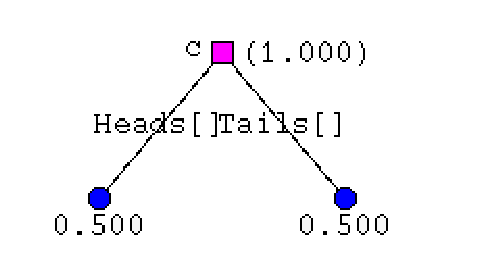
\includegraphics[scale=.6]{images/headOrTails.eps}
}
\caption{\lqpl{} program to do a coin flip}\label{fig:defsec:coin}
\end{figure}

In the function \inlqpl{cflip},  a \qbit{} is prepared by initializing it
to \ket{0} and applying the \Had{} transform. This creates a \qbit{} 
whose density matrix is {\begin{singlespace}$\begin{pmatrix}.5&.5\\ 
.5&.5\end{pmatrix}$\end{singlespace}}. When
 this \qbit{} is measured, it has a $50\%$ chance of being $0$ and 
an equal chance of being $1$. 

In the branches of the measure,  different values are assigned to the 
return variable $c$. Each of these assignments happens with a probability of
$50\%$. Once the measure statement is completed, the variable \inlqpl{c}
will be \inlqpl{Heads} and \inlqpl{Tails} each with a probability of $50\%$.
In the quantum stack machine this is represented as in 
sub-figure b of \vref{fig:defsec:coin}.


This illustrates the largest difference between quantum and classical 
processing of choices. In classical programming languages, a choice such
as a case type statement 
\emph{will only execute the code on one of the branches of the case}. 
In \lqpl{}, \emph{every} branch may be executed.


%\begin{wrapfigure}{l}{3in}
\begin{figure}[htbp]
\centering
\subfloat[Balanced creation]{
\begin{singlespace}
\lstinputlisting[style=linqpl]{examplecode/dataCreationExample1.qpl}
\end{singlespace}}
\qquad
\subfloat[Unbalanced creation]{
\begin{singlespace}
\lstinputlisting[style=linqpl]{examplecode/dataCreationUnbalanced.qpl}
\end{singlespace}}
\caption{\lqpl{} programs contrasting creation}
\label{fig:defsec:balancedcreation}
\end{figure}

When writing the dependent blocks of \inlqpl{measure}
 (and \inlqpl{case} in \vref{subsec:casestatements}) 
 variable creation must be
the same in each dependent list of statements.
 The compiler will give you a semantic
warning if a variable is created in one branch and not another.

For example, consider \vref{fig:defsec:balancedcreation}. In the left 
hand program on the 
\inlqpl{measure} starting at line \ref{line:measure1}, each branch creates a 
variable named '\inlqpl{i}'. This is legal and from line \ref{line:iexists}
forward,  '\inlqpl{i}' will be available.

On the other hand, the measure in the right hand program  starting in line 
\ref{line:measure2} assigns to the variable  '\inlqpl{c}' in
the \ket{0} branch and  '\inlqpl{d}' in the \ket{1} branch. At line
\ref{line:neitherdorc}, neither variable will be available. The compiler
will give the warnings:
\begin{quote}
\footnotesize
\terminalio{Warning: Unbalanced creation, discarding c of type INT}\\
\terminalio{Warning: Unbalanced creation, discarding d of type INT}
\end{quote}

\paragraph{Syntax of the \inlqpl{measure} statement.} This statement
starts with the word \emph{measure}, 
followed by a variable name, which must be of type \inlqpl{Qbit}. 
Next, the keyword \emph{of} signals the start of the two case selections.
 The case selection starts with either \ket{0} or \ket{1}, followed by
$=>$ and the block of dependent statements.

Note that \emph{both} case selections for a \qbit{} must be present. However,
it is permissible to not have any statements in a block.

\subsection{Case statement}\label{subsec:casestatements}
The \inlqpl{case} statement is used with any variable of a declared
datatype. 
\begin{figure}[htbp]
\begin{singlespace}
\lstinputlisting[style=linqpl]{examplecode/reverse.qpl}
\end{singlespace}
\caption[Reverse program to demonstrate \inlqpl{case}]{\lqpl{} program demonstrating \inlqpl{case}, a function to reverse a list.}
\label{fig:defsec:reverse}
\end{figure}  


In \vref{fig:defsec:reverse}, the program declares the
 \inlqpl{List} data type, which is parametrized by one
type variable and has two constructors: \inlqpl{Nil} which has no
arguments and \inlqpl{Cons} which takes two arguments of types
\inlqpl{a} and \inlqpl{List a} respectively.

The function \inlqpl{reverse} takes a list 
as an input argument and returns a single list, which is the original 
list in reverse order. Because of the linearity of the language
the original input list is not in scope at the end of the function.
The function \inlqpl{reverse} delegates to the function \inlqpl{rev'}
which uses an accumulator to hold the list as it is reversed.

The case statement begins on line \ref{line:rev:caserev}. For
\inlqpl{Nil}, it assigns the accumulator to the return list. For
\inlqpl{Cons}, it first adds the current element to the
front of the accumulator list, then it uses a recursive call
to reverse the tail of the original list with the new accumulator.


\begin{figure}[htbp]
\begin{singlespace}
\lstinputlisting[style=linqpl]{examplecode/treeMaxDepth.qpl}
\end{singlespace}
\caption[Tree depth program to demonstrate \inlqpl{case}]{\lqpl{} program demonstrating \inlqpl{case}, a function to compute the max tree depth.}
\label{fig:defsec:treemaxdepth}
\end{figure}

Considering the example in \vref{fig:defsec:treemaxdepth}. \inlqpl{TTree}
is a parametrized data type which depends on 
the type variable \inlqpl{a}. It
 has three constructors: \inlqpl{Tip} which takes no arguments;
\inlqpl{Br} which takes three arguments of types \inlqpl{TTree a, a} and
\inlqpl{TTree a}; and \inlqpl{Node} which takes one argument of type
\inlqpl{a}.

In \inlqpl{treeMaxDepth}, the case statement on line
\ref{line:flattenTree:casedepth} illustrates a ``don't care'' pattern for
both the \inlqpl{Node} and \inlqpl{Br} constructors. This function
 returns the maximum depth of the \inlqpl{TTree} and actually
discards  the actual data elements stored at nodes.



\paragraph{Syntax of the \inlqpl{case} statement.} This statement
starts with the word \emph{case}, 
followed by a variable   of some declared type.
Next, the keyword \emph{of} signals the start of the case selections.
The number of constructors in a type determine how many 
case selections the statement has. There is one selection 
for each constructor.
Each case selection consists of  a \emph{constructor pattern}, a
'$=>$' and dependent statements. 

Constructor patterns 
are the constructor followed by a parenthesized list of 
variables and / or \emph{don't care} symbols, '\_'.  Non-parametrized 
constructors appear without a list of variable names. The 
don't care symbol causes data to be discarded.

\subsection{Use and classical assignment statements}\label{subsec:usestatements}

The \inlqpl{use} statement is used with any variable of type \inlqpl{Int}
or \inlqpl{Bool}. 
This statement  has a single 
set of dependent statements. These may 
either be explicitly attached to the \inlqpl{use} statement or implicit.
Implicit dependent statements are all the statements following
the \inlqpl{use} until the end of the current block. 

Classical assignment is grouped here as it is syntactic sugar for a
\inlqpl{use} with implicit statements. This is illustrated in 
\ref{fig:useequalsassignment}.

%\begin{wrapfigure}{l}{2.75in}
\begin{figure}[htbp]
\begin{singlespace}
\begin{center}
\begin{tabular}{lcl}
$\vdots$ & & $\vdots$ \\
\begin{lstlisting}
i := exp;
s1;
\end{lstlisting} &
$\equiv$ &
\begin{lstlisting}
i = exp;
use i;
s1;
\end{lstlisting} \\
$\vdots$ & & $\vdots$
\end{tabular}
\end{center}
\end{singlespace}
\caption{Syntactic sugar for \inlqpl{use} / classical assignment}
\label{fig:useequalsassignment}
\end{figure}

The three types of classical use are semantically equivalent, but
do have different syntaxes as illustrated in \vref{fig:defsec:usestatements}.

\begin{figure}[htbp]
\centering
\subfloat[Explicit dependence]{
\begin{singlespace}
\lstinputlisting[style=linqpl]{examplecode/treeMaxDepth.explicit.frag.qpl}
\end{singlespace}}
\qquad
\subfloat[Implicit dependence]{
\begin{singlespace}
\lstinputlisting[style=linqpl]{examplecode/treeMaxDepth.frag.qpl}
\end{singlespace}}
\qquad
\subfloat[Classical assign]{
\begin{singlespace}
\lstinputlisting[style=linqpl]{examplecode/treeMaxDepth.cassign.frag.qpl}
\end{singlespace}}
\caption{Fragments of \lqpl{} programs contrasting \inlqpl{use} syntax}
\label{fig:defsec:usestatements}
\end{figure}

In sub-figure (a) of \ref{fig:defsec:usestatements}, the \inlqpl{use}
statement starts on line \ref{line:tmdfragexplicit:use}. The next two
statements are explicitly in its scope, which ends at line 
\ref{line:tmdfragexplicit:scopend}.  In sub-figure (b) of the same figure,
the \inlqpl{use} at line \ref{line:tmdfrag:use} is implicit. Its scope
extends to line \ref{line:tmdfrag:scopend}. Finally, in sub-figure(c),
the same effect is achieved with two classical assignments at 
lines \ref{line:tmdfragcas:assignj} and \ref{line:tmdfragcas:assignk}.
The scope of these assignments extend to line \ref{line:tmdfragcas:scopend}.


Unlike data types and \inlqpl{Qbit}s, which have a maximum number of 
sub-stacks, an \inlqpl{Int} has the potential to have 
 an unbounded number of values and therefore sub-stacks. 
The dependent statements of
 the \inlqpl{use} statement are executed for \emph{each} 
of these values.

To execute different pieces of code depending on the value, \lqpl{}
provides the \inlqpl{if} - \inlqpl{else} statement as discussed in
\vref{subsec:classicalcontrolstatements}.

\paragraph{Syntax of the \inlqpl{use} statement.} This statement starts with 
the word \inlqpl{use},
 followed by a list of variable names, which must be  of
type \inlqpl{Int} or \inlqpl{Bool}. If there is an 
explicit dependent block for the statement, it is given by the
keyword \inlqpl{in} followed by the dependent block.

When the \inlqpl{use} statement is \emph{not} followed by a dependent block, 
the rest of the statements in the enclosing block are considered in
the scope of the \inlqpl{use}.

Classical assign syntax is a variable name, followed by the 
symbol ':=' followed by an expression. The expression must have
type \inlqpl{Int} or \inlqpl{Bool}. 

\subsection{Function calls}\label{subsec:functioncalls}
Function calls include calling functions defined in  programs and
the predefined transforms. The list of predefined transforms valid
in a \lqpl{} program are given in \vref{tab:lqpltransforms}.
%TODO - Dr. C regarding transforms
% - reduce primitives, show how to get rest
% - Explain interdependence
% - reexamine formula for Rot, possibly use R(n,t) (t  an int), = 1 &0\\0&e^{-i t \pi / 2^{n-1}}
% - Remove RhoZ, Phase, T (Rot...) and Swap (=, =)
\begin{table}
\centerline{
\begin{tabular}{|l|l|c|}
\hline
\textbf{\lqpl{}}& \textbf{A.K.A.} & \textbf{Matrix} \\
\hline 
& & \\
\inlqpl{Not} & $X$, Pauli-X, $\rho_X$  & $ 
\begin{bmatrix}
0&1\\
1&0
\end{bmatrix}$ \\ & & \\\hline
 & &  \\
\inlqpl{RhoY} & $Y$, Pauli-Y, $\rho_Y$ &
$ 
\begin{bmatrix}
0&-i\\
i&0
\end{bmatrix}$ \\ & & \\\hline
 & &  \\
\inlqpl{RhoZ (=Rot(0))} & $Z$, Pauli-Z, $\rho_Z$ &
$ 
\begin{bmatrix}
1&0\\
0&-1
\end{bmatrix}$ \\ & & \\\hline
 & &  \\
\inlqpl{Had} & Had, $H$ &
$ 
\frac{1}{\sqrt{2}}\begin{bmatrix}
1&1\\
1&-1
\end{bmatrix}$ \\ & & \\\hline
& & \\
\inlqpl{Swap} & Swap &
$ 
\begin{bmatrix}
1&0&0&0\\
0&0&1&0\\
0&1&0&0\\
0&0&0&1
\end{bmatrix}$ \\ & & \\\hline
& & \\
\inlqpl{Phase (=Rot(2))} & $S$, Phase $\sqrt{Z}$ &
$
\begin{bmatrix}
1&0\\
0&i
\end{bmatrix}$ \\ & & \\\hline
& & \\
\inlqpl{T(=Rot(3))} & $T$, $\frac{\pi}{8}$, $\sqrt{S}$ &
$
\begin{bmatrix}
1&0\\
0&e^{i\pi/4}
\end{bmatrix}$ \\ & & \\\hline
& & \\
\inlqpl{Rot(n)} & $R_n$, Rotation &
$
\begin{bmatrix}
1&0\\
0&e^{i\pi/2^{n-1}}
\end{bmatrix}$ \\ & & \\\hline
\end{tabular}
} 
\caption{\lqpl{} transforms}\label{tab:lqpltransforms}
\end{table}

In addition to the predefined transforms, \lqpl{}
 allows you to prefix any of the 
predefined transformations with the 
string \inlqpl{Inv-} to get the inverse transformation. Controlled versions 
of all of these are available by using the quantum control construction
as defined in \vref{subsec:quantumcontrol}.
 For example,  the \inlqpl{Toffoli3} gate
as shown in \vref{tab:qgatesAndRep} is simply a  controlled-controlled-Not 
transformation.

The signatures of transforms are dependent upon the size of the 
associated matrix. A $2\times 2$ matrix gives rise to the signature
\inlqpl{(q:Qbit ; q:Qbit)}. In general, a $2^n \times 2^n$ matrix
will require $n$ \qbit{}s in and out. The parametrized transforms such
as \inlqpl{Rot} will  require one or more integers as input.

\subsubsection{Syntax of function calls}\label{subsubsec:syntaxfunction}
There are three different calling syntaxes for functions:
\begin{enumerate}
\item{} \emph{Functional} --- $(y_1,\dots,y_m) = f(n_1,\dots,n_k\, |\, x_1,\dots,x_j).$
\item{} \emph{Procedural} ---  $f(n_1,\dots,n_k\, |\, x_1,\dots,x_j\, ;\, y_1,\dots,y_m).$
\item{} \emph{Transformational} --- $f(n_1,\dots,n_k )\ z_1\ z_2\ \dots\ z_j.$
\end{enumerate}


\paragraph{Functions with classical and quantum inputs.}
These functions  may be called\footnote{A function
call with a  single unparenthesized variable appears on the
left hand side of the equals
 are
 actually assignment statements. The  right hand side of the assignment 
is a function expression.
See \vref{subsec:expressioncalls}} in each of the
three ways.
\begin{lstlisting}
      f ::(c1:Int,c2:Int, c3:Int | q1:Qbit, i1:Int ; a:Qbit, b:Int)
      = { ... }
      ...
         (a,b) = f(c1,c2,c3 | q1,i2);
         f(c1,c2,c3 | q1,i2; a,b);
         f(c1,c2,c3) q i;
\end{lstlisting}

When a function is called in the transformational syntax, as on the last 
line of the above code, the arguments (\inlqpl{q i} in the example) are 
both passed into
the function as arguments and used as return variables. 
The arguments in the parenthesis ( \inlqpl{c1,c2,c3} in our example),
\emph{must} be classical and a
 semantic error will result if a quantum variable is used.
If the number of in and out quantum arguments are not the same
or their types
do not match, this syntax is not available.


\paragraph{Functions which have no quantum input arguments.}
Functions which have only classical  inputs 
may be called in either the functional or procedural 
syntax. As there are no input quantum arguments, transformational
syntax is not allowed.

\begin{lstlisting}
      g :: (c1:Int, c2:Int | ; r:Int, d:Int) 
      = { ... }
      ...
        (a,b) = g(c1,c2 |);
        g(c1,c2 | ; a,b);
\end{lstlisting}


\paragraph{Functions which have no classical input arguments.}
Functions having only quantum  inputs may use
all three syntaxes. In this case, where the classical
variable list of arguments is empty, the ``|'' may 
be eliminated in procedural or functional calling, and the 
parenthesis may be eliminated in transformational calling.

\begin{lstlisting}
      h :: (q1:Int, q2:Int ; r:Int, d:Int) 
      = { ... }
      ...
        (a,b) = h(|c,d);
        (a,b) = h(c,d);
        h(|a,b ; c,d);
        h(a,b; c,d);
        h a b;
\end{lstlisting}



\paragraph{Linearity of function call arguments.}
Each input argument is no longer in scope after the function call. If 
the input is a simple identifier, the same identifier may be used in
the output list of the function. The transformational
syntax uses this technique to leave the variable names unchanged.

\paragraph{Syntactic forms of function and transform calls.}
In all three of the forms for function calling, the number and type
of input arguments must agree with the definition of the function.
Output identifiers must agree in number and their type is set according
to the definition of the functions output parameters. Output
variables are always quantum.

The  \emph{functional} syntax for function calling has three parts.
The first part is a parenthesized  list of variable names separated by 
commas.
The parenthesized list is then followed by an equals sign. The right hand side
 consists of the function name
followed by the  parenthesized  input arguments. The input arguments 
consists of two lists of arguments separated by '\inlqpl{|}'. The first
list consists of the classical arguments, the second of the quantum arguments.
Each argument must be a valid expression as defined 
in  \vref{sec:lqplexpressions}.
 If there are no classical arguments, the '\inlqpl{|}' is optional.


The  \emph{procedural} syntax for function calling starts with the
function name, followed by a parenthesized grouping of input and
output arguments.  As in the functional form, the list of classical input 
arguments are separated from the quantum ones by '\inlqpl{|}', which may
be eliminated when there are no classical arguments. The input arguments
are separated from the output arguments by '\inlqpl{;}'. 

The \emph{transformational} syntax starts with the
function name followed  by a parenthesized list of classical
expressions and then by a series of identifiers, separated by white space.
A requirement for using this syntax is that the
number and types of the input and output quantum arguments must be the same. 
The identifiers will be passed as input to the function and will be
returned by the function. The parenthesis for the list of classical
expressions may be eliminated when there are no classical parameters.


Function calls may also be expressions, which is discussed in
\vref{subsec:expressioncalls}.

\subsection{Blocks}\label{subsec:blocks}
Blocks are created by surrounding a list of statements with braces. A 
block may appear wherever a statement does.  All of the ``grouping''
types of statements require blocks rather than statements as their group.
See, for example, the discussion on \inlqpl{case} statements
in \vref{subsec:casestatements}.

\subsection{Quantum control}\label{subsec:quantumcontrol}

Quantum control provides a general way to create and use controlled unitary 
transforms in an \lqpl{} program. 
An example of quantum 
control is shown in the prepare and teleport functions in
 \vref{fig:defsec:stmts:demoofcontrol}.


\begin{figure*}[htbp]
\begin{singlespace}
\lstinputlisting[style=linqpl]{examplecode/teleport.qpl}
\end{singlespace}
\caption{\lqpl{} program demonstrating quantum control}
\label{fig:defsec:stmts:demoofcontrol}
\end{figure*}

\paragraph{Syntax of quantum control}
In \lqpl{} any statement, including block statements and 
procedure calls may be quantum controlled.
Semantically, this will  affect all transforms that occur within
the controlled statement, including
any of the transforms in a called function.
The  syntax is \emph{statement} 
followed by the symbols \emph{<=}, followed
by a list of identifiers.  These identifiers may 
be of any type, but are typically
either \qbit{}s or constructed data types with \qbit{} elements, such as a 
\inlqpl{List(Qbit)}.

The identifiers that are controlling a statement can not be used
in the statement. Controlling identifiers are exempt from
linearity constraints in that they remain in scope after the
quantum control construction.

The effect of the control is that all \qbit{}s in the 
control list, or contained in items
in that list are used to control all unitary 
transformations done in the controlled
statement.

\subsection{Divergence}\label{subsec:nontermination}
To force the execution  of a program  to diverge, you can use the
\inlqpl{zero} statement. This will set the probability of the values of
a program to 0, and is interpreted as non-termination.

\subsection{Discard}\label{subsec:discard}
In some algorithms, such as  in recursive functions when they process
the initial cases of constructed data,
the algorithm does not specify any action. In these cases, the programmer
may need to examine the requirements of linearity with respect to 
any passed in parameters. Often, these will need to be explicitly
discarded in base cases of such algorithms.
This is done via the discard statement.
An example may be seen in \vref{fig:inverserotate}.
\section{\lqpl{} expressions}\label{sec:lqplexpressions}

Expressions in \lqpl{} are used in many of the statements discussed in
\vref{sec:lqplstatements}. The four basic types of expressions are
identifiers, constants, constructor expressions, and calling expressions.
Arithmetic and logical combinations of classical 
constants and classical identifiers
are allowed. As well, constructor and calling expressions often  take 
lists of other expressions as arguments.

\subsection{Constant expressions}\label{subsec:constantexpressions}
The possible constant expressions in \lqpl{} are shown in 
\vref{tab:constantexpressions}. The category column in this table
contains the word ``Classical'' when the constant may be used in arithmetic
or Boolean expressions.

\begin{table}[htbp]
\begin{center}
\begin{singlespace}
\begin{tabular}{|l|l|l|}
\hline
\textbf{Expression} & \textbf{Type} & \textbf{Category} \\
\hline
\hline 
\emph{integer} & \inlqpl{Int} & Classical \\
& & \\
\inlqpl{true} & \inlqpl{Bool} & Classical \\
& & \\
\inlqpl{false} & \inlqpl{Bool} & Classical \\
& & \\
\inlqpl{|0>} & \inlqpl{Qbit} & Quantum \\
& & \\
\inlqpl{|1>} & \inlqpl{Qbit} & Quantum \\
\hline
\end{tabular}
\end{singlespace}
\end{center}
\caption{Allowed constant expressions in \lqpl}
\label{tab:constantexpressions}
\end{table}

\subsection{Identifier expressions}\label{subsec:identifierexpressions}
These expressions are just the identifier name. While an 
identifier may be used wherever an expression is expected, the reverse is not
true. As an example, in function calls, any of the input arguments may be
expressions but the output arguments \emph{must} be identifiers.

Identifier expressions may be either quantum or classical in nature. 
As discussed in \vref{subsec:assignmentstatement}, an identifier is 
first created by an assignment statement. When initially created, the
identifier is always quantum. Using it where a classical expression is 
required will result in an error. When it is desired to operate on an
identifier classically, it must first be the object 
of a  \inlqpl{use} statement.
In all statements in the scope of that \inlqpl{use} statement
the identifier will be considered classical. See \vref{subsec:usestatements}
for further information and examples.

\subsection{Constructor expressions}\label{subsec:constructorexpressions}
These expressions are used to create new instances of declared data types.
Consider this sample fragment of code.

{\begin{singlespace}
\begin{lstlisting}
        qdata TTree a = {Tip | Br ((TTree a), a, (TTree a)) | Node a}
        qdata List a = {Nil | Cons (a, (List a))}

        qbtree = Br(Tip, |1>, Br (Node(|0>),|1>,Node(|1>)));
        intlist = reverse(Cons(5,Cons(4,Cons(3,Cons(2,Cons(1,Nil))))));
\end{lstlisting}
\end{singlespace}
}

These statements create a tree as in \vref{fig:treeExample} and 
the list $[1,2,3,4,5]$. Compare the logical representation of
\inlqpl{qbtree} as in \ref{fig:treeExample} versus how it is stored
in the quantum stack machine, shown in \ref{fig:treeExampleInQS}
\begin{figure}[htbp]
\begin{center}
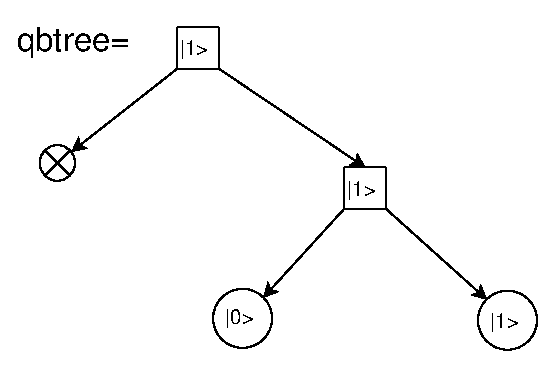
\includegraphics[scale=.6]{images/treeExample.eps}
\end{center}
\caption{Pictorial representation of \inlqpl{qbtree}}\label{fig:treeExample}
\end{figure}
\begin{figure}[htbp]
\begin{center}
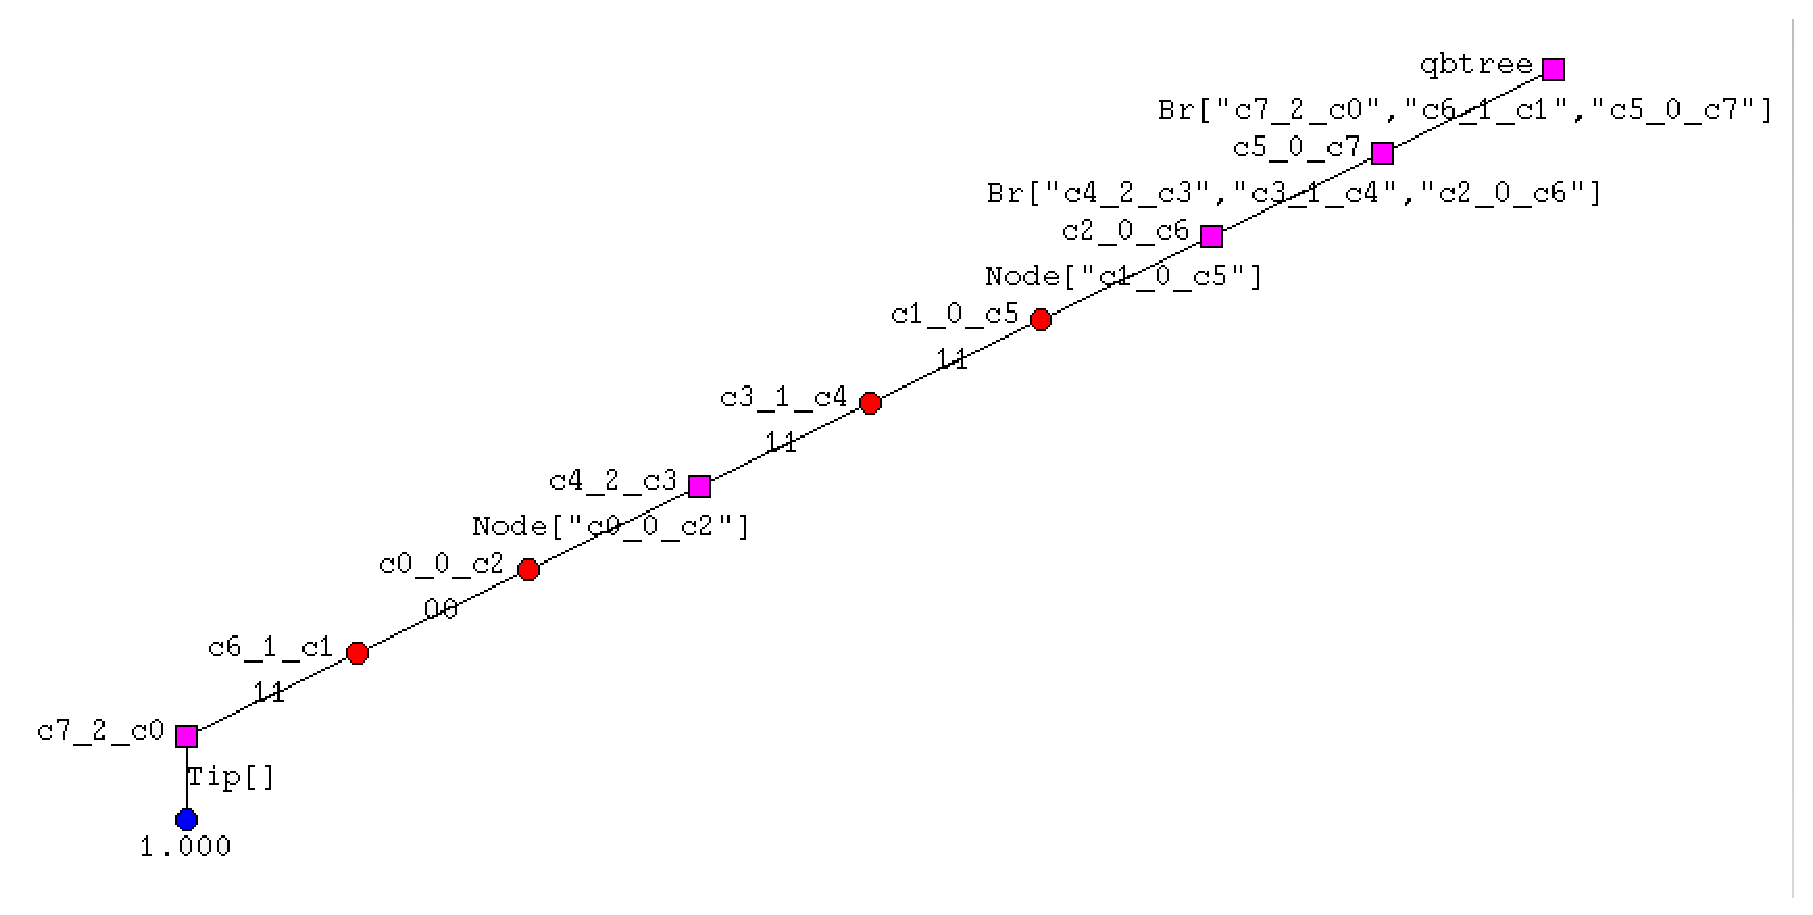
\includegraphics[scale=.5]{images/treeExampleInQS.eps}
\end{center}
\caption{Quantum stack contents after creation of \inlqpl{qbtree}}\label{fig:treeExampleInQS}
\end{figure}
The assignment statement which creates \inlqpl{qbtree} uses five constructor
expressions. The second assignment statement, which creates 
\inlqpl{intlist} uses six constructor expressions and one function expression.
% The extent of the constructor expressions are shown by the underlines here.
% {\begin{multline*}\footnotesize
%\shoveleft{\mathtt{qbtree =} 
%\underline{\mathtt{Br(}\underline{\mathtt{Tip}}\mathtt{,\ket{1},}
%\underline{\mathtt{Br(}\underline{\mathtt{Node(\ket{0})}}
%\mathtt{,\ket{1},}
%\underline{\mathtt{Node(\ket{1})}})})}; }\\
%\shoveleft{\mathtt{intlist =} 
%\mathtt{reverse(}\underline{\mathtt{Cons(5,}
%\underline{\mathtt{Cons(4,}
%\underline{\mathtt{Cons(3,}
%\underline{\mathtt{Cons(2,}
%\underline{\mathtt{Cons(1,}
%\underline{\mathtt{Nil}}\mathtt{)}}\mathtt{)}}\mathtt{)}}\mathtt{)}}\mathtt{)}}\mathtt{)};}
%\end{multline*}
% }

Constructor expressions either have no arguments
 (e.g. \inlqpl{Tip}, \inlqpl{Nil} above), or
require a parenthesized list of expressions which agree in both
number and type with the template supplied at the declaration of the
type. These expressions are unrestricted otherwise. They may be constants,
identifiers, other constructor expressions, expression calls or compound
expressions. Any expressions that are classical in nature, such as constants,
are upgraded to quantum automatically.

\subsection{Function expressions}\label{subsec:expressioncalls}
When a function returns a single value, it may be used in a
function expression. The bottom two lines of listing below shows
two examples of function expressions. 
\begin{lstlisting}
      f ::(c1:Int,c2:Int, c3:Int | q1:Qbit, i1:Int ; out:Qbit)
      = { ... }
      ...
         qout = f(c1,c2,c3 | q1,i2);
	 qlist = Cons(f(1,2,3 | qout, 5),Nil);
\end{lstlisting}
In the first function expression, \inlqpl{f} is the right hand side of 
an assignment statement. The assignment statement
 creates the variable \inlqpl{qout}
with the value returned by the function.

In the second function expression, \inlqpl{f} is the first argument of a 
constructor expression which will create a one element \inlqpl{List(Qbit)}.
The constructor expression is part of an assignment statement which
creates the variable \inlqpl{qlist} and sets it to
the one element list. Note that due to linearity, the variable 
\inlqpl{qout} is no longer available after the second function expression.

A function expression is always a quantum expression, so it may only be
used in those places where quantum expressions are allowed. Nesting of
these calls inside constructor expressions, other function expressions
and function calls is allowed.

\begin{figure}[htbp]
\lstinputlisting[style=linqpl]{examplecode/append.qpl}
\caption{\lqpl{} code for appending two lists}\label{fig:appendtwolists}
\end{figure}

In \vref{fig:appendtwolists}, line \ref{line:append:funcexp} shows the 
\inlqpl{append} being used as a function expression inside of a
constructor expression.

%\section{Linearity of \lqpl}\label{sec:lqpllinearity}
The language \lqpl{} treats all quantum variables as \emph{linear}. This 
means that any variable \emph{may only be used once}. 

\subsection{Linearity of quantum variables}\label{subsec:linearityofqvs}
Our primary reason for implementing this is the underlying aspect of 
linearity of quantum systems, as in the \emph{no-duplication} rule, 
which must be respected at all times. This allows us to provide
compile-time checking that enforces this rule.

The compiler and language do
 provide ways to ``ease the burden'' of linear thinking. 
For example, function calls provide a specialized syntax for variables
which are both input and output to a function. 

 - in intro now.
%\section{Operational semantics for the language \lqpl}
\label{sec:operationalsemanticslqpl}
In this section, I provide an operational semantics of \lqpl.
\subsection{Syntactic sets}\label{subsec:opsyntacticsets}
\lqpl{} has a variety of different syntactic sets as it is a quantum 
language with classical features. Traditional syntactic sets are composed
of unique elements, such as $N$ being the natural numbers. In \lqpl, the
base elements are sets of (value,probability) pairs, where the sum
of the probabilities is less than or equal to one. (A probability sum 
being strictly less than one signifies a chance of non-termination). 
This is required as
quantum operations, when a measure is applied, will create results of 
varying probabilities.

Certain items in the language are uniquely valued, for example, a constant.
In these cases, the constant will evaluate to the number it represents with
$100\%$ probability.

In the following list of syntactic sets, $p$ is always a probability
value between $0$ and $1$ inclusive. The required syntactic sets are:
\begin{itemize}
\item{} \n, the set of sets of $(n,p)$ pairs, where $n$ is an integer.
\item{} \T, the set of sets of $(t,p)$ pairs, 
where $t \in \{TRUE, FALSE\}$.
\item{} \Q, the set of quantum values as a single $2\times2$ matrix. ??????
\item{} \Data, the set of sets of $(d,p)$ pairs, where $d$ is a
defined constructor and associated items. 
\item{} \Qloc, the set of quantum locations.
\item{} \Cloc, the set of classical locations.
\item{} \Aexp, the set of arithmetic expressions.
\item{} \Bexp, the set of Boolean expressions.
\item{} \Cexp, the set of constructor expressions.
\item{} \Stm, the set of statements.
\end{itemize}

Following common practice, various letters will be used to range over these
sets. Sub-scripting and adding of primes to the letter does not change the 
category they belong to.
\begin{itemize}
\item{} $(n,p),(m,p)$ for \n.
\item{} $q,r$ for \Q.
\item{} $(d,p)$ for \Data.
\item{} $Z,Q$ for \Qloc.
\item{} $X,Y$ for \Cloc.
\item{} $a$ for \Aexp.
\item{} $b$ for \Bexp.
\item{} $c$ for \Cexp.
\item{} $e$ for $\Aexp + \Bexp + \Cexp$.
\item{} $s$ for \Stm.
\end{itemize}

The execution of statements in \lqpl, while functional, may be thought of
as a function from a state to the next state. That state is composed of the
disjoint 
union of the elements in \n, \T, \Q{} and \Data. This set is denoted as 
\R. Additionally, \Loc{} will denote the disjoint union of 
\Cloc{} and \Qloc{}. $r$ will range over \R{} and $L$ over \Loc{} 
where required.
The \emph{state} $\Sigma$ of a 
program at a particular point is a function
 $\sigma: \Loc \to\R$.

As operational semantics are an \emph{evaluation} based semantics,
the evaluation of a pair consists of an item in one of our 
expression sets(\Aexp, \Bexp{} and \Cexp)
 and a state to a value in one of the base sets(\n,\T, \Q{} and \Data).
I denote this evaluation triplet by:
\[\eval{e}{\sigma}{r}.\]

\subsection{Operational semantics of arithmetic expressions}\label{subsec:oparithmetic}
All rules that follow are presented in the premise / conclusion format.
\subsubsection{Constants and variables}
\[\infer[\mathrm{numbers}]{\eval{n}{\sigma}{(n,1.0)}}{}\]
\[
\infer[\mathrm{Classical}]{\eval{X}{\sigma}{\sigma(X)}}{}
\qquad
\infer[\mathrm{Quantum}]{\eval{Z}{\sigma}{\sigma(Z)}}{}
\]
\subsubsection{Binary operations}
\[
\infer[{n=n_0+n_1}]{\eval{a_0 + a_1}{\sigma}{(n,p_0 \times p_1)}}
    {\eval{a_0}{\sigma}{(n_0,p_0)}\quad\eval{a_1}{\sigma}{(n_1,p_1)} }
\]
\[
\infer[{n=n_0-n_1}]{\eval{a_0 - a_1}{\sigma}{(n,p_0 \times p_1)}}
    {\eval{a_0}{\sigma}{(n_0,p_0)}\quad\eval{a_1}{\sigma}{(n_1,p_1)} }
\]
\[
\infer[{n=n_0\times n_1}]{\eval{a_0 * a_1}{\sigma}{(n,p_0 \times p_1)}}
    {\eval{a_0}{\sigma}{(n_0,p_0)}\quad\eval{a_1}{\sigma}{(n_1,p_1)} }
\]
\[
\infer[{n=n_0 \div n_1}]{\eval{a_0 / a_1}{\sigma}{(n,p_0 \times p_1)}}
    {\eval{a_0}{\sigma}{(n_0,p_0)}\quad\eval{a_1}{\sigma}{(n_1,p_1)} }
\]
\[
\infer[{n=n_0 - (n_1 \times (n_0 \div n_1))}]{\eval{a_0 \bmod a_1}{\sigma}{(n,p_0 \times p_1)}}
    {\eval{a_0}{\sigma}{(n_0,p_0)}\quad\eval{a_1}{\sigma}{(n_1,p_1)} }
\]
\[
\infer[{n=n_0 \times 2^{n_1}}]{\eval{a_0 <\!< a_1}{\sigma}{(n,p_0 \times p_1)}}
    {\eval{a_0}{\sigma}{(n_0,p_0)}\quad\eval{a_1}{\sigma}{(n_1,p_1)} }
\]
\[
\infer[{n=n_0 \div 2^{n_1}}]{\eval{a_0 >\!> a_1}{\sigma}{(n,p_0 \times p_1)}}
    {\eval{a_0}{\sigma}{(n_0,p_0)}\quad\eval{a_1}{\sigma}{(n_1,p_1)} }
\]


\subsection{Operational semantics of Boolean expressions}\label{subsec:opboolean}

\subsubsection{Constants and variables}
\[\infer{\eval{\true}{\sigma}{(\true,1.0)}}{}
\qquad
\infer{\eval{\false}{\sigma}{(\false,1.0)}}{}
\]
\[
\infer[\mathrm{Classical}]{\eval{X}{\sigma}{\sigma(X)}}{}
\qquad
\infer[\mathrm{Quantum}]{\eval{Z}{\sigma}{\sigma(Z)}}{}
\]
\subsubsection{Binary operations}
\[
\infer[\mathrm{when\ }n\mathrm{\ and\ }m\mathrm{\ are\ equal}]
     {\eval{a_0 = a_1}{\sigma}{(\true,p_0 \times p_1)}}
    {\eval{a_0}{\sigma}{(n,p_0)}\quad\eval{a_1}{\sigma}{(m,p_1)} }
\] Redone in chap 3
%\section{Examples of programs for the quantum stack machine}\label{sec:examples}
% Move examples into code.
\chapter{The quantum stack machine}\label{chap:quantumStackMachine}
\section{Introduction to the quantum stack machine}\label{sec:introStackMachine}
The quantum stack machine provides an execution environment where
 quantum and classical data may be manipulated. The primary component
of this machine is the \emph{quantum stack}, which stores both quantum and
probabilistic data.

The quantum stack  has the same function as a  classical stack 
in that it provides the basic
operations and data structures
 required for quantum computation. 
\Ref{chap:semantics} initially showed how quantum circuits can be
interpreted as acting on  a simple quantum stack consisting
of \bits{} and \qbits. Later sections of \ref{chap:semantics}
extended the quantum stack with datatype and classical data nodes,
together with operations on those nodes. \Ref{sec:semanticsiteration}
gave the interpretation of recursive functions acting on a quantum stack.

This chapter  describes a machine using this full quantum stack and other
data structures to provide an execution environment for \lqpl{} programs.


\section{Quantum stack machine in stages}\label{sec:qsmstate}
The quantum stack machine is described in terms of four 
progressively more elaborate stages. The first stage is
the   \emph{basic QS-machine}, labelled \bms. This stage provides
 facilities for the majority of operations
of our machine, including classical operations, adding and discarding data
 and classical control. The second stage, the \emph{labelled QS-machine},
called \lbms{} adds the capability of applying 
unitary transforms with the modifiers 
\semins{Left, Right} and \semins{IdOnly} as introduced in 
\ref{sec:programmingaquantumstack}. 
The third stage, the  \emph{controlled QS-machine}, is labelled \cms{} and 
provides the
ability to do quantum control. The final stage,  the
\emph{QS-machine}, is labelled \ms{} and 
 adds the ability to call subroutines and do 
recursion.

These stages are ordered in terms of complexity and the
operations definable on them. The ordering is:
\[ \bms < \lbms < \cms < \ms\]
When a function is defined on one of the lower stages, it is possible
to lift it to a function on any of the higher stages. 
The details of the Haskell implementation of 
these stages and the lifting functions are given in 
\vref{subsec:QSM:machinedescription}.

\subsection{Basic quantum stack machine}\label{subsec:basicmachinestate}

The quantum stack machine transitions for the quantum instructions 
 are defined  at this stage.
The state of the basic quantum stack machine  has a code stream, $\cd$, a
classical stack, $S$, a  quantum stack, $Q$, a dump, $D$ and a
name supply, $N$.
\begin{equation}
(\cd,S,Q,D,N)\label{eq:minimalmachinestate} \\
\end{equation}

The code, $\cd$,  is a list of machine instructions. Transitions 
effected by these instructions are detailed in 
 \vref{subsec:transitiondiagrams}. English descriptions of the
instructions and what they do are given in 
 \vref{subsec:repauxinstructions}.


The classical stack, $S$, is a standard stack whose items may
be pushed or pulled onto the top of the stack and specific locations 
may be accessed for both reading and updating.
Classical arithmetic and Boolean operations are done with the top
elements of the classical stack. Thus, an add will pop the
top two elements of the classical stack and then push the result 
 on to the top of the stack.


The dump, $D$, is a holding area for intermediate results and returns. This
is used when measuring quantum bits,  using probabilistic data, 
splitting constructed data types and for calling subroutines. Further
details are given in \vref{sec:representationofdump}.


The name supply, $N$, is an integer that is incremented each
time it is used. The name supply is used when binding nodes to 
constructed data nodes. As they are bound, they are renamed to a unique name
generated from the name supply. For further details on this, see 
the transitions for \qsmins{QBind} at \vref{subsec:quantumstacknodecreation}.

\subsection{Labelled quantum stack machine}\label{subsec:labelledmachinestate}

The labelled QS-machine, \lbms, extends  \bms{} by
labelling the quantum stack, $L(Q)$. The quantum stack is labelled to 
control the application of
 unitary transformations, which allows quantum control to
be implemented.

The labelled QS-machines state is a tuple of five elements:
\begin{equation}
(\cd,S,L(Q),D,N)\label{eq:minimalmachinestateplus}
\end{equation}

The quantum stack is labelled by one of four labels: 
\emph{Full, RightOnly, LeftOnly} or 
\emph{IdOnly}. These labels 
describe how unitary transformations will be applied to  the quantum stack.

When this labelling was introduced in \ref{sec:programmingaquantumstack}, it 
was used as an instruction modifier rather than a labelling of the
quantum stack. While the implementation of these modifiers  is
changed, the effect on the quantum stack is the same. The quantum stack
machine transitions for unitary transformations are detailed 
in  \vref{subsec:trans:unitarytransformations}.


\subsection{Controlled quantum stack machine}\label{subsec:controlledmachinestate}

The controlled quantum stack machine, \cms, adds the capability to 
 add or remove quantum control.
This stage  adds a control stack, $C$, and changes the 
 tuple of classical stack, labelled quantum stack, dump
and name supply into a  list of tuples of these elements. In the 
machine states, a list will be denoted by enclosing the list items
or types in square brackets.

The \cms{} state is a tuple of three elements, where the third element
is a list of four-tuples:
\begin{equation}
(\cd, C , [(S,L(Q),D,N)]) \label{eq:controlmachinestate}
\end{equation}



The control stack is implemented using 
a list of functions, each of which is defined on the third element of
\cms. The functions in the control stack
transform the list of  tuples $(S,L(Q),D,N)$.  Control points are
added to the control stack 
by placing an identity function at the top of
the stack. Control points are removed by taking the top of the control stack
and applying it to the current third element of \cms, resulting in
a new list of tuples.
Adding a \qbit{} to control will modify the function on top of the control
stack
and change the list of tuples of $(S,L(Q),D,N)$.

\subsection{The complete quantum stack machine}\label{subsec:machinestate}

The complete machine, \ms,  allows the  implementation of  subroutine calling.
Its state consists of 
an infinite list of \cms{} elements.

\begin{equation}
\Inflist{(\cd, C , [(S,L(Q),D,N)])} \label{eq:machinestate}
\end{equation}


Subroutine calling is done in an iterative manner. At the head of the
infinite list, no subroutines are called, but result in divergence.
Divergence is represented in the quantum stack machine by a quantum 
stack with a trace of $0$.

In the next position of the infinite list, a subroutine will be entered once.
If the subroutine
 is recursive or calls other subroutines, those calls will diverge. 
The next position of the infinite list will call one more
level. At the $n^{\mathrm{th}}$ position of the infinite list 
subroutines are executed to a call depth of $n$.

\subsection{The classical stack}\label{subsec:repauxclassicalstack}
The machine uses and creates values
on the classical stack when performing arithmetic operations. 
This object is a standard 
push-down stack with random access.
Currently it accommodates both integer and Boolean values.

\subsection{Representation of the dump}\label{sec:representationofdump}
When processing various operations in the machine, such as  those
labelled as quantum control (measure et. al.), the machine will 
need to save intermediate stack states and results. To illustrate, when 
processing a case deconstruction of a datatype,
the machine saves all partial trees of the node on the dump together
with an empty stack to accumulate
 the results of processing these partial trees.
After processing  each case the current quantum stack is
merged with the result stack and the next partial stack is processed. 
The classical stack is also saved in the
dump element at
the beginning of the process and reset to this saved value 
when each case is evaluated.


The dump is  a list of \emph{dump elements}. There are two distinct types
of dump elements, one for quantum control instructions and one used for
  call statements. The details of these elements may
be found in the description of the quantum control transitions in
 \vref{subsec:measurementandchoice} and 
function calling in \vref{subsec:functioncalling}.

\subsection{Name supply}
The name supply is a read-only register of the machine. It 
provides a unique name
when binding nodes to a data node. The implementation 
uses an integer value which
is incremented for each of the variables in a selection pattern in
a case statement. It is reset to zero at
the start of each program.

%\section{Transforming between the states}\label{sec:statetransforming}

As introduced in \vref{sec:qsmstate}, there are four different 
state descriptions for the transition diagrams.
They are:
\begin{gather*}
\bms = (\cd,S,Q,D,N)\\
\bms' = (\cd,S,L(Q),D,N)\\
\cms = (\cd, C , [(S,L(Q),D,N)])\\
\ms = \il{(\cd, C , [(S,L(Q),D,N)])} 
\end{gather*}

These actual states are used in the Haskell implementation for the 
quantum stack machine. In that implementation, 
\vref{subsec:QSM:machinedescription}  gives the 
details of the  higher order functions which
lift a function on one of the base states (\bms, \bms', \cms) to the 
machine state (\il{(\cd, C , [(S,L(Q),D,N)])}).

\subsection{Lifting functions on \bms{} to \bms'.}\label{subsec:liftbmstobmsprime}
An endomorphism of \bms{} is changed to an endomorphism of \bms{}' by 
ignoring the labelling. That is, lifting of the endomorphism is accomplished
by commuting it
with the labelling. So, if
\[ f\,(\cd,S,Q,D,N) = (\cd_f,S_f,Q_f,D_f,N_f)\]
then 
\[ (\text{lift}\ f)(\cd,S,L(Q),D,N) = (\cd_f,S_f,L(Q_f),D_f,N_f).\]


\subsection{Lifting functions on \bms{}' to \cms}\label{subsec:liftbmstocms}
This sub-section describes how to lift a restricted type of
 endomorphism on $\bms' = (\cd,S,L(Q),D,N)$ to
an endomorphism on $\cms = (\cd, C , [(S,L(Q),D,N)])$.

When moving from \bms{}' to \cms, the lifting of the function maps it 
across the list of tuples in \cms, while ignoring the control object $C$. We
require one restriction on the endomorphism for this to work. 
The restriction is that the code result of the endomorphism 
only depends on the code of the input. That is,
given $f::\bms' \to\bms'$ where
 $f (\cd,S,L(Q),D,N) = (\cd_f,S_f,L(Q)_f,D_f,N_f) $ then
$\cd_f = f_1(\cd)$ for some function $f_1$.

The lifting function that does this is defined in a series of smaller steps.
First, consider
$(\cd, C , [(S,L(Q),D,N)])$, an
object in \cms. This can be transformed to
\[(C,[(\cd,S,L(Q),D,N)])\]
by duplication $\cd$ and ``pasting'' it in front of each tuple in the list.
Given the endomorphism $f$ of $\bms'$, it may now be applied to each of 
the elements of the list, as each of them is an object in \bms'. 

Since  $f$ is restricted as above, it is allowed to reverse
the ``pasting'' and bring the code portion out of the list of tuples. As
each code portion was equal before 
applying $f$ and the code result
only depends on the code input for $f$, 
it is safe to simply use the code from the
first tuple in the list. Removing the code entry from all of the other tuples
 completes the transformation back to an  object of \cms.


\subsection{Lifting functions on \cms{} to \ms}\label{subsec:liftcmstoms}
This sub-section describes how to lift an
 endomorphism on  $\cms = (\cd, C , [(S,L(Q),D,N)])$ to 
an endomorphism on $\ms = \il{(\cd, C , [(S,L(Q),D,N)])}$.

The final stage, from \cms{} to \ms{}, makes use of the fact that
the infinite list functor is known to be a monad. Thus, 
the Kleisli lifting will transform any endomorphism in \cms{} to an
endomorphism in \ms{}.

Infinite lists are given by the co-inductive type 
defined with the destructors $\hd$, which returns the base type, and
$\tl$, which returns a new infinite list.
\[\ila=\nu x.\{\hd: A, \tl: x\}\]
Categorically this corresponds to the diagram in \vref{fig:inflistalgebra} 
which defines infinite lists.
\begin{figure}[htbp]
\[
\xymatrix{
A \ar@{=}[d] &
    C \ar[l]_{h} \ar[r]^{t} \ar@{.>}[d]^{f}&
    C \ar@{.>}[d]^{f}\\
A &
    \ila \ar[l]^{\hd} \ar[r]_{\tl}&
    \ila
 }
\]
\caption{Initial algebra diagram for infinite lists}\label{fig:inflistalgebra}
\end{figure}

Recall that for a monad, given the functor $T$, (which is $\il{\_}$ in
this case) the natural transformations 
$\eta::I\to T, \mu::T^2\to T$ so that the
diagrams in \vref{fig:opstandardmonad} commute must be supplied.
\begin{figure}[htbp]
\[
\xymatrix{
T^3 \ar[r]^{T\mu} \ar[d]_{\mu T} &
    T^2 \ar[d]^{\mu} \\
T^2 \ar[r]_{\mu} &
    T
 }\quad \mathrm{\ and\ }\quad
\xymatrix{
IT \ar@{=}[dr] \ar[r]^{\eta T} &
    T^2 \ar[d]^{\mu} &
    TI \ar[l]_{T\eta} \ar@{=}[dl]\\
 & T &
 }
\]
\caption{Standard monad coherence diagrams}\label{fig:opstandardmonad}
\end{figure}

In the case of the infinite list, $\mu=$\emph{diagonal} 
and $\eta=$\emph{constant}, that is:
\begin{gather*}
\mu([[a_{00},a_{01},\ldots],[a_{10},a_{11},\ldots],\ldots]) = 
[a_{00},a_{11},a_{22},\ldots] \\
\eta(a) = [a,a,a,\ldots]
\end{gather*}

What this means is that for any endomorphism in \cms, it is  lifted to \ms{}
 by
just applying it across the entire infinite list. When composing these with 
native endomorphisms of \cms{} (in the quantum stack machine, 
only the \qsmins{Call} instruction generates
one of these), composition is done by
 taking the diagonal of the resulting infinite list of infinite lists.
\TODO{ - seems a bit light....} Note about transforming added to Intro.
\section{Representation of data in the quantum stack}\label{subsec:representationofqstackdata}

The quantum stack was introduced and described in \ref{chap:semantics}. This
section will give further details of the implementation of the quantum
stacks and show example nodes.

\subsection{Representation of \qbit{}s.}\label{subsec:representationOfQbits}
A single \qbit{} is represented on the quantum stack as a  node with
four possible branches. This assumes a basis for quantum computation
of two elements, which is identified with $(0,1)$ and $(1,0)$ in 
 $\complex^2$. The four possible values of the branches represent
the elements of the \qbit{}'s density matrix. This is illustrated in
\vref{fig:lqplHadQbit}. From left to right, the branches are labelled with
$00, 01, 10$ and $11$. The value at each branch is $.5$. This 
corresponds to the density matrix {\begin{singlespace}
$\begin{bmatrix}.5&.5\\.5&.5\end{bmatrix}$\end{singlespace}
}

\begin{figure}[htbp]
\centerline{
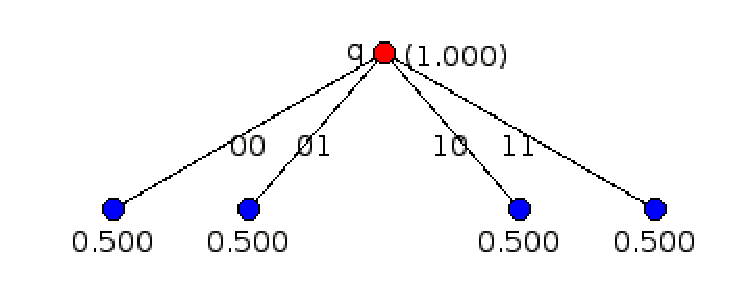
\includegraphics[scale=.6]{images/HadQbit.eps}
}
\caption{A \qbit{} after a \Had{} transform}\label{fig:lqplHadQbit}
\end{figure}

With multiple \qbit{}s,  the representation becomes hierarchical.
For example, two \qbit{s} will be represented by a tree with one of the
\qbits{} at the top and each of its sub-branches
 having the second \qbit{} below it. 
Consider applying a Hadamard transform to one \qbit, followed by a 
controlled-Not with that \qbit{} as the control. This is 
a standard way to entangle two \qbits. As illustrated in
\vref{fig:entangled}, this creates a tree in the quantum stack with
a total of four non-zero leaves. The quantum stack in the figure
corresponds to a sparse representation of the density matrix:

{\begin{singlespace}
\[\left[
\begin{array}{c|c}
\begin{array}{cc}
.5&0\\0&0
\end{array} &
\begin{array}{cc}
0&.5\\0&0
\end{array}\\
\hline
\begin{array}{cc}
0&0\\.5&0\\
\end{array} &
\begin{array}{cc}
0&0\\0&.5
\end{array}
\end{array}\right]
\]
\end{singlespace}
}

\begin{figure}[htbp]
\centerline{
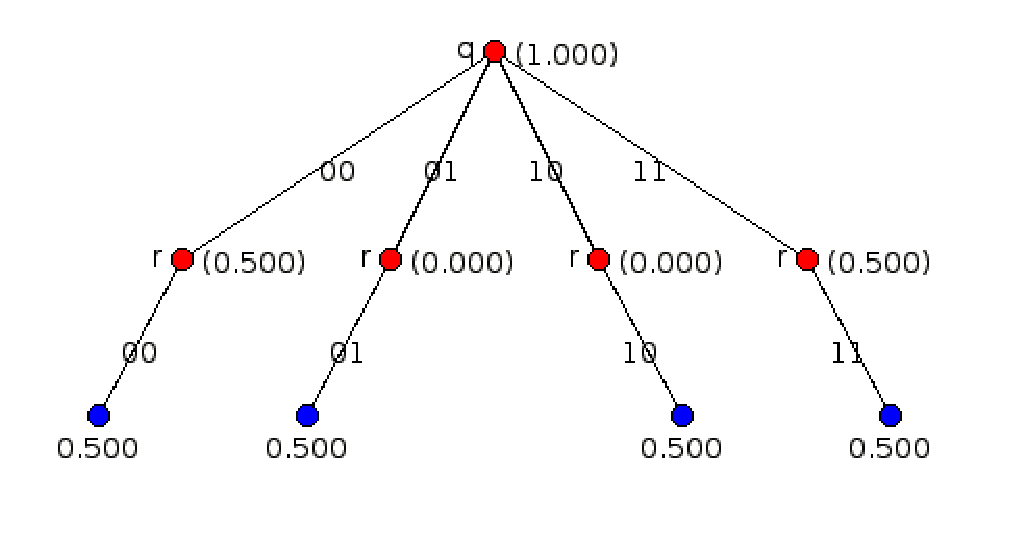
\includegraphics[scale=0.6]{images/entangledQbits.eps}
}
\caption{Two entangled \qbits}\label{fig:entangled}
\end{figure}

\subsection{Representation of integers and Boolean values}\label{subsec:representclassicaldata}
Numeric and Boolean
 data in the quantum stack machine is represented by a node with
a sub-branch for each value that occurs with a non-zero probability. 
These values may be of either integer or Boolean type.

\begin{figure}[htbp]
\centerline{
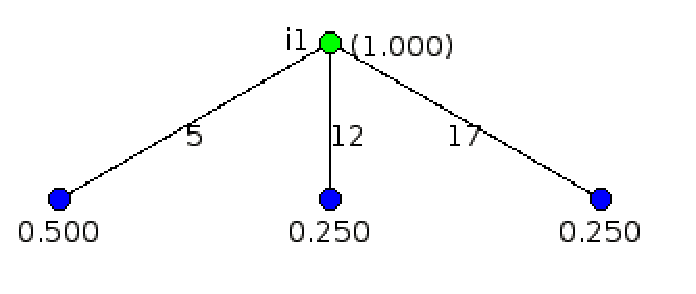
\includegraphics[scale=.6]{images/integer.eps}
}
\caption{An integer with three distinct values}\label{fig:integerofthree}
\end{figure}

\Vref{fig:integerofthree} depicts an
integer $i1$ which has 
a $50\%$ probability of being $5$, and $25\%$ each of being $12$ or $17$.

\subsection{Representation of general data types}\label{subsec:representgeneraldatatyps}
The general datatype is represented 
as a node with one branch for each of the constructors that occurs
with a non-zero probability. Each branch is labelled by the 
constructor and the names of any nodes that are 
bound to it\footnote{For example, in \qtype{List}s of 
integers, the
\qcons{Cons} constructor requires a base integer and another \qtype{List}.}.
These
nodes will be referred to as  \emph{bound nodes}.


\begin{figure}[htbp]
\centerline{
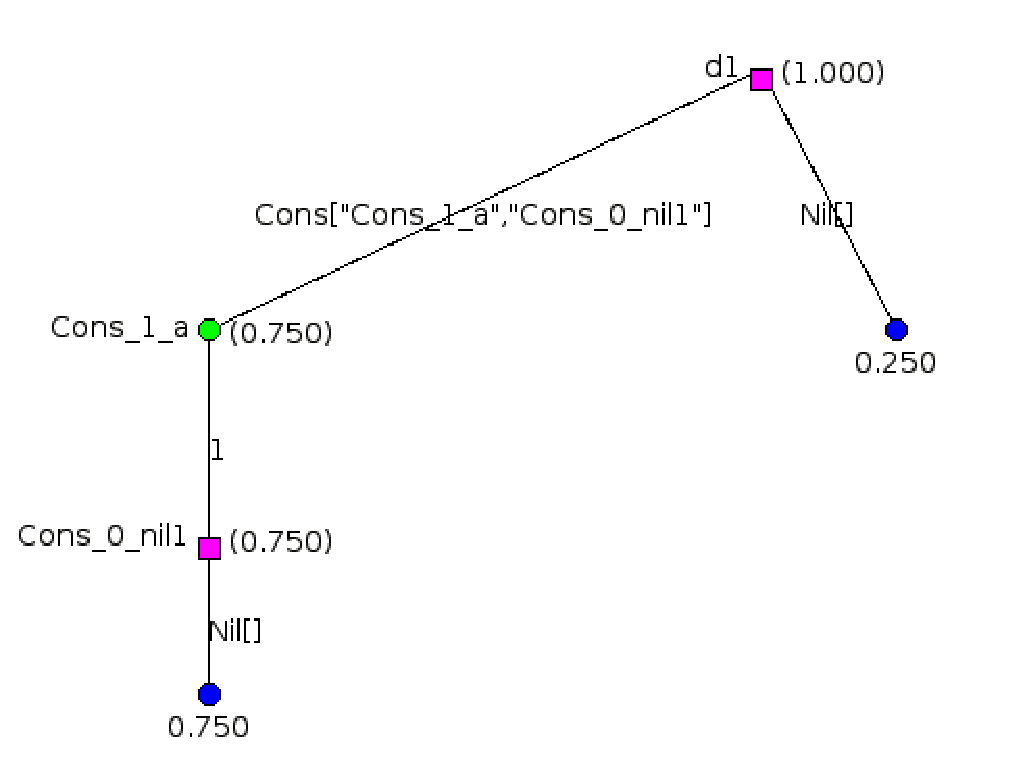
\includegraphics[scale=.5]{images/listExample.eps}
}
\caption{A list which is a mix of $[\ ]$ and $[1]$.}\label{fig:schizolist}
\end{figure}



For example, in the \qtype{List} that appears in \vref{fig:schizolist}, 
the top node  is a mix of values. The node $d1$ has a $25\%$ chance of 
being \qcons{Nil} and $75\%$ of being a \qcons{Cons} of two bound nodes.
The first bound node is an element of the base type, integer. 
It is labelled \terminalio{Cons\_1\_a} which
is an integer node having the single value 1. The second bound element is 
\terminalio{Cons\_0\_nil1},  which is another list having the
 single value of \qcons{Nil}. 





\section{Quantum stack machine operation}\label{sec:stackmachineoperation}
This section describes the actual transitions of the stack
machine for each of the instructions in the machine.

\subsection{Machine transitions}\label{subsec:transitiondiagrams}
The majority of the transitions presented in this section are 
defined on 
a machine of type $\bms = (\cd,S,Q,D,N)$ as was 
introduced in \vref{subsec:basicmachinestate}.
As discussed in that section, labelling only affects the
transition of unitary transforms. All other instruction transitions 
ignore it, giving us:
\[ Ins(L(Q)) = L (Ins (Q)) \]
where $Ins$ is the transition of some other instruction.

The transition for the application of transformations will use \lbms, while
the transition for the add/remove control instructions 
uses the machine state of  \cms. 
The call instruction uses the 
state of the complete machine, \ms, which allows recursion.
All of these stages and their associated states were defined and discussed 
in  \vref{sec:qsmstate}.



\subsection{Node creation}\label{subsec:quantumstacknodecreation}
There are three instructions which allow us to create data on the 
stack and one which binds sub-nodes into a data type. These are 
\qsmins{QLoad, QCons, QMove} and \qsmins{QBind}. The transitions are shown
in \vref{fig:trans:nodeconstruction}.

The instructions do the following tasks:
\begin{description}
\item{\qsminswithp{QLoad}{nm\ \ket{i}}} --- Load a new \qbit{} named 
\qsminsparm{nm} on top of the quantum stack with the value \ket{i};
\item{\qsminswithp{QCons}{nm\ Cns}} -- Load a new datatype node on top of the
quantum stack with name \qsminsparm{nm} and value \qsminsparm{Cns}.
Sub-nodes are not bound  by this instruction.
\item{\qsminswithp{QMove}{nm}} --- Load a new classical node on top of the
quantum stack with name \qsminsparm{nm} and value taken from the
top of the classical stack. If the classical stack is empty, the
value is defaulted to $0$.
\item{\qsminswithp{QBind}{nm}} --- Binds a sub-node down the 
branch of the node to the datatype constructor on top of the 
quantum stack. Furthermore, the act of binding will
cause the newly bound sub-node to be renamed so that it is
hidden until an unbind is performed. \qsmins{QBind} 
uses the name supply,
$N$, to create the new  name for the sub-node. The machine will
generate an exception if the top of the quantum stack is not a
single branched datatype or if a node named \qsminsparm{nm} is not found. 
\end{description}


\begin{figure}[htbp]
\begin{tabular}{l}
$(\mathrm{QLoad}\ x\ \ket{k}{:}\cd,S,Q,D,N)  $ \\
$ \trspace\implies(\cd,S,x{:}[\ket{k}\to Q],D,N)$ \\
$(\mathrm{QCons}\ x\ c{:}\cd,S,Q,D,N) $ \\
$ \trspace\implies (\cd, S,x{:}[c\{\}\to Q],D,N) $ \\
$ (\mathrm{QMove}\ x{:}\cd,v{:}S,Q,D,N) $ \\
$ \trspace\implies (\cd,S,x{:}[\bar{v}\to Q],D,N)$ \\
$(\mathrm{QBind}\ z_0{:}\cd,S,x{:}[c\{z_1',\ldots,z_n'\}\to Q],D,N) $\\
$ \trspace \implies (\cd,S,x{:}[c\{z(N),z_1',\ldots,z_n'\}\to Q[z(N)/z_0]],D,N') $
\end{tabular}
\caption{Transitions for node construction}\label{fig:trans:nodeconstruction}
\end{figure}



\subsection{Node deletion}\label{subsec:nodedeletion}

Three different instructions, \qsmins{QDelete, QUnbind} and \qsmins{QDiscard}
 remove data from the 
quantum stack.  These instructions are the converses of \qsmins{QBind}, 
\qsmins{QLoad} and \qsmins{QMove}. Their transitions are shown in
\ref{fig:trans:nodedestruction} and \ref{fig:trans:noderemoval}.
The instructions do the following tasks:
\begin{description}
\item{\qsmins{QDelete}} --- removes the top node of the stack 
\emph{and any bound sub-nodes}. This instruction has no restrictions on
the number of sub-stacks or bindings in a data node;
\item{\qsmins{QDiscard}} --- removes the top node of the stack. In all cases,
the top node can only be removed when it has
a single sub-stack. For datatype nodes, \qsmins{QDiscard} also requires
there are no bound sub-nodes.
\item{\qsminswithp{QUnbind}{nm}} --- removes the
 first bound element from a data type 
\emph{provided it has a single sub branch}. The datatype node must be
 on top of the quantum stack. The newly unbound sub-node is renamed
 to \qsminsparm{nm}.
\end{description}


\begin{figure}[htbp]
\begin{tabular}{lll}
$(\mathrm{QDelete}{:}\cd,S,Q{:}[\ket{k_{ij}}\to Q_{ij}],D,N)$&$ \implies $&$(\cd,S,(Q_{00}+Q_{11}),D,N)$ \\[12pt]
$(\mathrm{QDelete}{:}\cd,S,DT{:}[c_i\{b_{ij}\} \to Q_i],D,N)$&$ \implies $&$(\cd,S,\sum_i(del(\{b_{ij}\}, Q_i)),D,N)$ \\[12pt]
$(\mathrm{QDelete}{:}\cd,S,I{:}[\overline{v}_i \to Q_i],D,N)$&$ \implies $&$(\cd,S,\sum_i Q_i,D,N)$ 
\end{tabular}
\caption{Transitions for destruction}\label{fig:trans:nodedestruction}
\end{figure}

For the \qsmins{QDelete} instruction, the type of node is irrelevant.
It will delete the node and, in the case of datatype nodes, any
bound nodes. This instruction is required to implement 
sub-routines that have parametrized datatypes as input arguments.
For example, the algorithm for determining the length of a
list is to return $0$ for the ``Nil'' constructor and 
add $1$ to the length of the tail list in the ``Cons'' constructor. 
When doing this, the elements of the list are deleted due to the 
linearity of \lqpl.
The compiler will have no way of determining the type of the 
elements in the list and
therefore could not generate the appropriate quantum split and discards.
The solution is to use a \qsmins{QDelete} instead.

The subroutine $del$ used in the transitions 
in \ref{fig:trans:nodedestruction}
will recursively rotate up and then delete the bound nodes of a datatype
 node.


\begin{figure}[htbp]
\begin{tabular}{lll}
$(\mathrm{QDiscard}{:}\cd,S,x{:}[\ket{k}\to Q],D,N) $&$ \implies$&$ (\cd,S,Q,D,N)$ \\[12pt]
$(\mathrm{QDiscard}{:}\cd,S,x{:}[c\{\} \to Q],D,N) $&$\implies $&$(\cd,S,Q,D,N)$ \\[12pt]
$(\mathrm{QDiscard}{:}\cd,S,x{:}[\overline{v} \to Q],D,N) $&$\implies$&$ (\cd,v{:}S,Q,D,N)$ \\[12pt]
\multicolumn{3}{l}{$(\mathrm{QUnbind}\ y{:}\cd,S,x{:}[c\{z_1',\ldots,z_n'\}\to Q],D,N) $} \\
\multicolumn{3}{r}{$\trbigspace\implies (\cd,S,x{:}[c\{z_2',\ldots,z_n'\} \to Q[y/z_1']],D,N)$}
\end{tabular}
\caption{Transitions for removal and unbinding}\label{fig:trans:noderemoval}
\end{figure}



 The 
renaming is an integral part of the \qsmins{QUnbind}
instruction, as a compiler will not be able to know  the bound names of
a particular data type node. The instruction 
does \emph{not} delete the data type at the top of the stack or
the unbound node. If the top node is not a data type or has more than
a single branch or does not 
have any bound nodes, the machine will generate an exception. 

The machine ensures that it does not create  name capture issues
by rotating the bound node to the top of the sub-stack before
it does the rename. That is, given the situation as depicted in
the transitions, the quantum stack machine performs the 
following operations:

{\begin{singlespace}
\begin{enumerate}
\item{} $ Q' \leftarrow pull(z_1',Q)$;
\item{} $ Q'' \leftarrow  Q'[y/z_1'] $;
\item{} $z_1'$ is removed from the list of constructors;
\item{} The new quantum stack is now set to $x{:}[c\{z_2',\ldots,z_n'\} \to Q'']$.
\end{enumerate}
\end{singlespace}
}



\subsection{Stack manipulation}\label{subsec:stackmanipulation}
Most operations on a quantum stack affect only the top of the stack.
 Therefore,  the machine must have
 ways to move items up the stack. This requirement is met by the instructions
\qsmins{QPullup} and \qsmins{QName}. The transitions are shown in 
\vref{fig:trans:manipulation}.

The instructions do the following tasks:
\begin{description}
\item{\qsminswithp{QPullup}{nm}} --- brings the \emph{first} node named 
\qsminsparm{nm} to the top of the quantum stack. 
It is not an error to try pulling up a non-existent address. The original
stack will not be changed in that case.
\item{\qsminswithp{QName}{nm_1\ nm_2}} --- renames the first
node in the stack having \qsminsparm{nm_1} 
to \qsminsparm{nm_2}.
\end{description}

\begin{figure}[htbp]
\begin{tabular}{lll}
$(\mathrm{QPullup}\ x{:}\cd,S,Q,D,N) $&$\implies$&$ (\cd,S,\mathrm{\textsf{pull}}(x,Q),D,N)$ \\[12pt]
$(\mathrm{QName}\ x\ y{:}\cd,S,Q,D,N) $&$\implies$&$ (\cd,S,Q[y/x],D,N)$ 
\end{tabular}
\caption{Transitions for quantum stack manipulation}\label{fig:trans:manipulation}
\end{figure}

A \qsminswithp{QPullup}{nm} has the potential to be
an expensive operation as the node \qsminsparm{nm} may be 
deep in the quantum stack . In practice, many
 pullups interact  with only the top two or three elements of the
quantum stack.

The algorithm for pullup is based on preserving the bag of 
\emph{path signatures}.  A {path signature} for a node
consists of a bag of ordered pairs (consisting of the node name and
the branch constructor) where
every node from the top to the leaf is represented. 
Pulling up a
node will reorder the sub-branches below nodes to keep this invariant.

Due to the way  arguments of recursive subroutines are handled in \lqpl,
it is actually possible to get multiple nodes with the same name, however, this
does not cause a referencing problem as only the highest such node is actually
available in the \lqpl{} program.

\subsection{Measurement and choice}\label{subsec:measurementandchoice}
The instructions
\qsmins{Split}, \qsmins{Measure} and \qsmins{Use} start the task of 
operating on a node's partial stacks, while the fourth, \qsmins{EndQC} 
is used to iterate through the partial stacks. The transitions are shown in 
\vref{fig:trans:measures}.

The instructions do the following tasks:
\begin{description}
\item{\qsminswithp{Use}{Lbl}} --- uses the classical node at the top
of the quantum stack and executes the code at \qsminsparm{Lbl} for
each of its values.
\item{\qsminswithp{Split}{(c_1,lbl_1),\dots,(c_n,lbl_n)}} --- uses the
datatype node at the top of the stack and
execute a jump to the code 
at \qsminsparm{lbl_i} when there is a branch having constructor
\qsminsparm{c_i}. Any constructors not mentioned in the instruction 
are removed from the node first. There is no ordering 
requirement on the pairs of constructors and labels in \qsmins{Split}.
\item{\qsminswithp{Measure}{Lbl_{00}\ Lbl_{11}}} --- using the
\qbit{} node on top of the quantum stack, executes
 the code at its two labels for 
 the \qsminsparm{00} and \qsminsparm{11} branches. 
The off-diagonal elements  of the \qbit{} will be
discarded. This implements a 
non-destructive measure of the \qbit.
\item{\qsmins{EndQC}} --- signals the end of processing of dependent 
instructions and begins processing the next partial stack.
 When all values are processed, merges the results and returns
to the instruction after the corresponding \qsmins{Measure}, \qsmins{Use}
or \qsmins{Split} instruction.
\end{description}

\begin{figure}[htbp]
\begin{tabular}{l}
$(\mathrm{Use}\ \lbl_U{:}\cd,S,x{:}[\bar{v_i}\to Q_i],D,N) $ \\
$\trspacetwo\implies (\mathrm{EndQC},S,0, 
	\dmpelemqc{}(S,[(x_i{:}v_i\to Q_i,\lbl_U)],\cdptr, 0){:}D,N)$ \\[12pt]
$(\mathrm{EndQC},S',Q,\dmpelemqc{}(S,
	[(x_i{:}v_i\to Q_i,\lbl_U)]_{i=j,\ldots,m},\cdptr, Q'){:}D,N) 
       $ \\
$\trspacetwo\implies (\lblcd_U,S,x_j, \dmpelemqc{}
	(S,[(x_i{:}v_i\to Q_i,\lbl_U)]_{i=j+1,\ldots,m},\cdptr,Q+Q'){:}D,N)$ \\[12pt]
$(\mathrm{EndQC},S',Q,\dmpelemqc{}(S,[],\cdptr, Q'){:}D,N) 
       $ \\
$\trspacetwo\implies (\cd,S,Q+Q', D,N)$\\[12pt]
\\
$(\mathrm{Split}\ [(c_i,\lbl_i)]{:}\cd,S,x{:}[c_i\{V_i\}\to Q_i],D,N) $ \\
$\trspacetwo\implies (\mathrm{EndQC},S,0, 
	\dmpelemqc{}(S,[(x_i{:}c_i\{V_i\}\to Q_i, \lbl_i)],\cdptr, 0){:}D,N)$ \\[12pt]
$(\mathrm{EndQC},S',Q,\dmpelemqc{}(S,[(x_i{:}c_i\{V_i\}\to Q_i, \lbl_i)]_{i=j,\ldots,m},\cdptr, Q'){:}D,N) 
       $ \\
$\trspacetwo\implies (\lblcd_j,S,x_j, \dmpelemqc{}(S,[(x_i{:}c_i\{V_i\}\to Q_i, \lbl_i)]_{i=j+1,\ldots,m},\cdptr,Q+Q'){:}D,N)$ \\[12pt]
$(\mathrm{EndQC},S',Q,\dmpelemqc{}(S,[],\cdptr, Q'){:}D,N) 
       $ \\
$\trspacetwo\implies (\cd,S,Q+Q', D,N)$\\
\\
$(\mathrm{Meas}\ \lbl_0\ \lbl_1{:}\cd,S,x{:}[\ket{0}\to Q_0,\ket{1}\to Q_1, 
    \ldots],D,N) $ \\
$\trspacetwo\implies (\mathrm{EndQC},S,0, 
       \dmpelemqc{}(S,[(x_k{:}\ket{k}\to 
	Q_k,\lbl_k)]_{k\in\{0,1\}},\cdptr, 0){:}D,N)$ \\[12pt]
$(\mathrm{EndQC},S',Q, \dmpelemqc{}(S,
	[(x_k{:}\ket{k}\to Q_k,\lbl_k)]_{k\in\{0,1\}},\cdptr, Q'){:}D,N) 
       $ \\
$\trspacetwo\implies (\lblcd_0,S,x_0,  
	\dmpelemqc{}(S,[(x_1{:}\ket{1}\to 
	Q_1,\lbl_1)],\cdptr,Q+Q'){:}D,N)$ \\[12pt]
$(\mathrm{EndQC},S',Q, \dmpelemqc{}(S,
	[(x_1{:}\ket{1}\to Q_1,\lbl_1)],\cdptr, Q'){:}D,N) 
       $ \\
$\trspacetwo\implies (\lblcd_1,S,x_1,  
	\dmpelemqc{}(S,[],\cdptr,Q+Q'){:}D,N)$ \\[12pt]
$(\mathrm{EndQC},S',Q,\dmpelemqc{}(S,[],\cdptr, Q'){:}D,N) 
       $ \\
$\trspacetwo\implies (\cd,S,Q+Q', D,N)$
\end{tabular}
\caption{Transitions for quantum node choices}\label{fig:trans:measures}
\end{figure}

Each of the code fragments pointed to 
by the instruction labels \emph{must} end with the instruction
\qsmins{EndQC}. The \qsmins{EndQC} instruction  will trigger execution
 of the code associated with the 
next partial stack. 


The \qsmins{QUnbind} is meant to be used at the start of the dependent
 code of a \qsmins{Split} instruction.
The  sequencing to process a datatype node is to
do a \qsmins{Split}, then in each of the dependent blocks, execute
\qsmins{QUnbind} instructions, possibly interspersed with 
\qsmins{QDelete} instructions when the bound node is not further used
in the code.
This is always concluded with a \qsmins{QDiscard} that discards the data node
which was the target of the \qsmins{Split}.

In the following discussion there are no significant differences between the
\qsmins{Split} and \qsmins{Measure}. The action of
\qsmins{Split} is described in detail.

The \qsmins{Split}, \qsmins{Measure} and \qsmins{Use}
 instructions make  use of the dump. The dump element
used by these instructions consists of four parts: 
\begin{itemize}
\item{}\emph{The return label}. This is used 
when the control group is complete.
\item{}\emph{The remaining partial stacks}. A list consisting 
of pairs of quantum stacks and 
their corresponding label. These partial stacks are the ones waiting
 to be processed by the control group. 
\item{}\emph{The result quantum stack}. This quantum stack 
 accumulates the merge result of 
processing each of the control groups partial stacks. This is initialized
to an empty stack with a zero trace.
\item{}\emph{The saved classical stack}. The classical stack is reset to this
value at the start of processing a partial stack and at the end. This 
occurs each time an \qsmins{EndQC} instruction is executed.
\end{itemize}


The instruction 
\qsminswithp{Split}{[(c1,l1),(c2,l2)]} starts by  creating a dump entry with
$[(c1\rightarrow Q_1,l1),(c2 \rightarrow Q_2,l2)]$ as the
list of partial stacks and label pairs. The 
dump entry will hold \qsminsparm{0} quantum stack as
the result stack, 
the current state of the classical stack  and the address of the 
instruction following the \qsmins{Split}.
The final processing of the 
\qsmins{Split} instruction sets the current quantum stack to 
zero and sets the next code 
to be executed to be \qsmins{EndQC}. 

The \qsmins{EndQC} will  change the top dump element
by removing the first pair $(c1\rightarrow Q_1, l1$) from the
execution list. It 
will set the current quantum stack to the first element of this
pair and the code pointer to the second element.
Execution then proceeds with the first instruction at $l1$.

When the next \qsmins{EndQC} instruction is executed, the dump will
again be changed. First the current quantum stack will be merged with
the result stack on the dump. Then the next pair of 
partial quantum stack $P_q\ (=c2\rightarrow Q_2) $ 
and code pointer $l2$ is removed from the execution list. 
The  current quantum stack is set to $P_q$ and the code pointer 
is set to $l2$. Finally, the classical stack is reset to the one 
saved in the dump element.

When the partial stack  list on the dump element is empty, 
the \qsmins{EndQC} instruction
will merge the current quantum stack with the result stack and then
set the current quantum stack to that result. 
The classical stack is reset to the one
saved on the dump, the code pointer is set to the return location
 saved in the
dump element and the dump element is removed. Program execution then
continues from the saved return point.

Normally, the first few instructions pointed to by the \qsminsparm{Label} in 
the pairs of constructor and code labels will unbind any bound nodes and 
delete the node at the top of the stack. 
QSM does not \emph{require} this, hence, it is possible to implement both
destructive and non-destructive measurements and data type deconstruction.

\paragraph{Using classical values.} The \qsmins{Use} instruction introduced
above differs from both \qsmins{Split} and \qsmins{Measure} in that it works
on a node that may an unbounded number of sub-nodes.
The \qsminswithp{Use}{lbl} instruction moves 
all the partial stacks to the quantum stack, one at a time, and then
executes the code at \qsminsparm{lbl}
 for the resulting machine states. Normally, this 
code will start with a \qsmins{QDiscard}, which will put the node
value for that partial stack onto the
classical stack, and finish with an  \qsmins{EndQC} to
 trigger the processing of the next partial stack.

The dump and \qsminsparm{EndQC} processing for a \qsminswithp{Use}{lbl}
 is the same
as for a \qsmins{Split} or \qsmins{Measure}. The execution list pairs
will all have the same label, the \qsminsparm{lbl} on the instruction.

\subsection{Classical control}\label{subsec:classicalcontrol}
The machine provides the three instructions \qsmins{Jump, CondJump} and
\qsmins{NoOp} for branch control. Jumps are allowed only in a
forward direction. The transitions for these are shown in 
\vref{fig:trans:classicalcontrol}. The instructions do the following tasks:
\begin{description}
\item{\qsminswithp{Jump}{lbl}} --- causes execution to continue with 
the code at \qsminsparm{lbl}.
\item{\qsminswithp{CondJump}{lbl}} --- examines the top of the classical stack. 
When it is \qsmfalse, execution will continue with 
the code at \qsminsparm{lbl}. If it is any other value, execution continues with
the instruction following the \qsmins{CondJump}.
\item{\qsmins{NoOp}} --- does nothing in the machine. Execution continues with 
the instruction following the \qsmins{NoOp}.
\end{description}

\begin{figure}[htbp]

\begin{tabular}{lll}
$(\mathrm{Jump}\ \lbl_J{:}\cd,S,Q,D,N) $&$\implies $&$ (\lblcd_J,S,Q,D,N)$ \\[12pt]
$(\mathrm{CondJump}\ \lbl_J{:}\cd, \qsmfalse{}{:}S,Q,D,N) $ &$\implies $&$ (\lblcd_J,S,Q,D,N)$ \\[12pt]
$(\mathrm{CondJump}\ \lbl_J{:}\cd, \qsmtrue{:}S,Q,D,N) $ &$\implies $&$ (\cd,S,Q,D,N)$ \\[12pt]
$(\mathrm{NoOp}{:}\cd, S,Q,D,N) $ &$\implies $&$ (\cd,S,Q,D,N)$ 
\end{tabular}
\caption{Transitions for classical control.}\label{fig:trans:classicalcontrol}
\end{figure}


 No changes are made to the classical stack,
the quantum stack or the dump by these instructions.
While \qsmins{NoOp} does nothing, it is allowed as the target of a jump. 
This is 
used by the \lqpl{} compiler in the  code generation 
 as the instruction following a \qsmins{Call}.


\subsection{Operations on the classical stack}\label{subsec:operationsonclassicalstack}
The machine has five instructions that affect the classical stack directly.
They are \qsmins{CGet, CPut, CPop, CApply} and \qsmins{CLoad}, with 
transitions shown in \vref{fig:trans:classicalops}. The instructions perform
the following tasks:
\begin{description}
\item{\qsmins{CPop}} --- destructively removes the top element of the
classical stack.
\item{\qsminswithp{CGet}{n}} --- copies the $n^{\text{th}}$ element of the 
classical stack to the top of the classical stack.
\item{\qsminswithp{CApply}{\mathrm{\textsf{op}}}} --- applies the operation \qsminsparm{op} to 
the top elements of the classical stack, replacing them with the result of 
the operation. Typically, the \qsminsparm{\mathrm{\textsf{op}}}
 is  a binary operation such as 
\emph{add}.
\item{\qsminswithp{CLoad}{v}} --- places the constant  \qsminsparm{v} on
 top  of the classical stack.
\end{description}

\begin{figure}[htbp]
\begin{tabular}{lll}
$(\mathrm{CPop} {:}\cd,v{:}S,Q,D,N) $ &$\implies  $ &$(\cd,S,Q,D,N)$ \\[12pt]
$(\mathrm{CGet}\ n {:}\cd,v_1{:}\cdots{:}v_n{:}S,Q,D,N)  $ &$\implies $ &$ (c,v_n{:}v_1{:}\cdots{:}v_n{:}S,Q,D,N)$ \\[12pt]
$(\mathrm{CPut}\ n {:}\cd,v_1{:}\cdots{:}v_n{:}S,Q,D,N)  $ &$\implies  $ &$(c,v_1{:}\cdots{:}v_1{:}S,Q,D,N)$ \\[12pt]
$(\mathrm{CApply}\ \mathrm{\textsf{op}}_n{:}\cd,v_1{:}\cdots{:}v_n{:}S,Q,D,N)  $ &$\implies  $ &$(\cd,\mathrm{\textsf{op}}_n(v_1,\ldots,v_n){:}S,Q,D,N)$ \\[12pt]
$(\mathrm{CLoad}\ n\ {:}\cd,S,Q,D,N) $ &$ \implies $ &$ (\cd,n{:}S,Q,D,N)$
\end{tabular}
\caption{Transitions for classical stack operations.}\label{fig:trans:classicalops}
\end{figure}

\subsection{Unitary transformations and quantum control}\label{subsec:trans:unitarytransformations}
The QS-Machine has three instructions which add or remove \qbits{} (and other nodes)
from quantum control. The instruction transitions in this group
are defined directly on \cms{} or \lbms,  
as they will either affect the control
stack (\qsmins{AddCtrl, QCtrl, UnCtrl}) or need to take into account
 the labelling of the quantum stacks (\qsmins{QApply}). 

The first three instructions do not affect the actual state
of the quantum stack, classical stack or dump.
The \qsmins{QApply} does affect the state of the quantum stack.
The transitions  are
shown in \vref{fig:trans:unitarytransform}.

 The instructions perform
the following tasks:
\begin{description}
\item{\qsmins{AddCtrl}} --- starts a new control point on the control stack.
\item{\qsmins{QCtrl}} --- adds the node at the top of the 
quantum stack, together
with any dependent sub-nodes to the control stack.
\item{\qsmins{UnCtrl}} --- removes \emph{all} the nodes in the top control
point of the control stack.
\item{\qsminswithp{QApply}{n\ T}} --- parametrized the transform 
\qsminsparm{T} with the top $n$ elements of the classical stack and
then applies the parametrized transform to quantum stack. Control is respected
because of the labelling of the quantum stack.
\end{description}

\begin{figure}[htbp]
\begin{tabular}{l}
$(\mathrm{AddCtrl}{:}\cd,C,[(S_i,L(Q_i),D_i,N_i)]_{i=1,\cdots n})]) $ \\
$\trspace\qquad\implies (\cd,id{:}C,[(S_i,L(Q_i),D_i,N_i)]_{i=1,\cdots n})])$\\[12pt]

$(\mathrm{QCtrl}{:}\cd,f{:}C,[(S_i,L(Q_i),D_i,N_i)]_{i=1,\cdots n})]) $ \\
$\trspace\qquad\implies (\cd,(g\circ f){:}C,[(S^{'}_j,L(Q_j)^{'},D^{'}_j)]_{j=1,\cdots m})])$\\[12pt] 
$(\mathrm{UnCtrl}{:}\cd, f{:}C,[(S_i,L(Q_i),D_i,N_i)]_{i=1,\cdots n})]) $ \\
$\trspace\qquad\implies (\cd,C,[(S^{''}_j,L(Q_j)^{''},D^{''}_j)]_{j=1,\cdots p})])$\\[12pt]
$(\mathrm{QApply}\ m\ t{:}\cd, (v_1{:}\cdots {:}v_m{:}S),L(Q),D,N)  $ \\
$\trspace\qquad\implies (\cd,S,
           \mathrm{\textsf{cTrans}}([v_1,\ldots,v_m],t,L(Q)),D,N)$ 
\end{tabular}
\caption{Transitions for unitary transforms}\label{fig:trans:unitarytransform}
\end{figure}

The function $cTrans$ in the transition for \qsmins{QApply} must first 
create the transform. In most cases, this is a fixed  transform (e.g., \nottr,
\Had), but both \inlqpl{rotate} and the \inlqpl{UM}
 transforms are parametrized. 
The transform  \inlqpl{rotate} is used in the quantum Fourier transform and 
\inlqpl{UM} is the $a^x \mod N$ transform used in order finding.

When the top node is a \qbit, the function expects its required number
of \qbits{} to be the top nodes. For example, a \Had{} expects only $1$, a 
$swap$ expects 2 and an \inlqpl{UM}
 will expect as many \qbits{} as $N$ requires
\bit{}s.

When the top node is a datatype node the machine will attempt to rotate up the 
required number of \qbits{} to the top, perform the operation and 
then re-rotate the datatype node back to the top. It will rotate the bound 
nodes of a datatype node starting at the 
 left and proceeding to the  right. Left to right is determined by the 
 ordering in the original constructor expression used to create
the datatype node. The machine will throw 
an exception if  there are insufficient bound nodes (e.g., 
\inlqpl{Nil} for a list) or if the rotation would be indeterminate. 
Indeterminacy happens whenever a subject datatype node has more than one
sub-stack.

Once this is accomplished the function will transform the top parts of
the stack into a matrix $Q$ of appropriate size ($2\times2$ for a $1-\qbit$ 
transform, $16\times16$ for a $4-\qbit$ and so forth) with entries
being the sub-stacks. 

At this point, the control labelling 
of the quantum stack is considered and one of
the following four transforms will happen. If the actual transform
is named $T$, the result will be:
\begin{equation}
\mathrm{cTrans}\ T\ L(Q) =
\begin{cases}
L(Q) & L= \mathrm{IdOnly}\\
L(T Q) & L= \mathrm{LeftOnly}\\
L(Q T^{*}) & L= \mathrm{RightOnly}\\
L(T Q T^{*}) & L= \mathrm{Full}
\end{cases}
\end{equation}

Following this the quantum stack is reformed from the resulting 
matrix. 

\subsection{Function calling and returning}\label{subsec:functioncalling}
The \qsmins{Call} and \qsmins{Return} instructions are used for 
function calling.
The \qsmins{Call} instruction is the only instruction that needs to 
directly work on \ms, the infinite list of \cms{} items. The transition
for this is defined in terms of a subordinate function \emph{enterF}
 which is 
defined on \bms. Its transition is also described below.

Recall the QS-machine stages have the states:
\begin{gather*}
\bms = (\cd,S,Q,D,N)\\
\cms = (\cd, C , [(S,L(Q),D,N)])\\
\ms = \Inflist{(\cd, C , [(S,L(Q),D,N)])} 
\end{gather*}
For the state \ms{}, an infinite list will be expressed as
\[H_0 \ilsep T = H_0 \ilsep H_1 \ilsep H_2 \ilsep \cdots\]
where $H$ is an element of the correct type for the infinite 
list.
 
 The instructions do the following tasks:
\begin{description}
\item{\qsminswithp{Call}{n\ lbl}} --- Calls the subroutine at \qsminsparm{lbl}, 
copying the top \qsminsparm{n} elements of the classical stack to a 
classical stack for the subroutine. 
\item{\qsminswithp{Return}{n}} --- Uses the return label in the
head of the dump to return from the subroutine. It also copies
 the top \qsminsparm{n} elements from the classical stack and
places them on top of the saved classical stack from the dump element.
\end{description}

\begin{figure}[htbp]
\begin{tabular}{l}
$ (\mathrm{Call}\ n\ \lbl_C{:}\cd,C, [(S_i,L(Q)_i,D_i,N_i)])_0 \ilsep T$\\
$\trspace\implies (\cd,C, [(S_i,L(\emptyset)_i,D_i,N_i)])_0 \ilsep
{lift\ (enterf\ n\ \lbl_C)\ T}$\\
$enterf\ n\ \lbl_C (\cd,v_1{:}\cdots{:}v_n{:}S,Q,D,N) $ \\
$\trspace\implies (\lblcd_C,[v_1,\ldots,v_n],Q,R(S,\cdptr){:}D,N)$ \\
$(\mathrm{Return}\ n,v_1{:}\cdots{:}v_n{:}S',Q,R(S,\cdptr){:}D,N) $ \\
$\trspace\implies (\cd,[v_1,\ldots,v_n]{:}S,Q,D,N)$ \\
\end{tabular}
\caption{Transitions for function calls.}\label{fig:trans:functioncalls}
\end{figure}

To illustrate how \qsmins{Call} is being processed, consider
the following diagram:
\begin{align*}
(0)&&M_0 &\ilsep &M_1 &\ilsep &M_2 &\ilsep &M_3 &\ilsep \dots \\
(1)&\ (\qsmins{Call}\ f):\quad&0 &\ilsep &f \cdot M_1 &\ilsep &f \cdot M_2 &\ilsep &f \cdot M_3 &\ilsep \dots \\
(2)&\ (\qsmins{Call}\ f):\quad&0 &\ilsep &0 &\ilsep &f \cdot f \cdot M_2 &\ilsep &f \cdot f \cdot M_3 &\ilsep \dots \\
(3)&\ (\qsmins{Call}\ f):\quad&0 &\ilsep &0 &\ilsep &0 &\ilsep &f \cdot f \cdot f \cdot M_3 &\ilsep \dots \\
&&&&&\vdots
\end{align*}

At the start, in line (0), the machine has state $M_0\ilsep M_i$. After the
first call to $f$, at line (1), 
the head of the infinite list state has been zeroed out, 
indicating divergence. However, at every position further down the
infinite list, the subroutine $f$ is entered.

Continuing to line (2) and calling $f$ again, the divergence has moved 
one position to the right and we now have a state of
 $0\ilsep 0\ilsep f \cdot f \cdot M_i$. Line (3) follows the same pattern.
 Thus, the further 
along in the infinite list one goes, the greater the \emph{call depth}.

 For  details of how this is
handled in the Haskell implementation of the quantum stack machine, 
see \vref{subsubsec:QSM:recursivefunctiontransitions}.

The \qsmins{Call} and \qsmins{Return} instructions use a dump element
as part of subroutine linkage.
The \qsminswithp{Call}{i\ lbl} instruction creates a dump element to store 
the 
current classical stack and the address of the instruction following
the \qsmins{Call} instruction. 
The \qsminswithp{Return}{n} instruction will use the top dump element
to reset the code pointer  to the saved return location.
\qsmins{Return} also takes the classical stack from the top dump element and the
top \qsminsparm{n} values from the current classical stack are added
to the top of it. \qsmins{Return} then removes the top dump element.


%\section{Abstract semantics of the quantum stack machine}
\label{sec:abstractsemanticsqsm}
This section  presents a categorical semantics for the
quantum stack machine introduced in this chapter.
\chapter{Future Work}\label{chap:futurework}
As with any piece of research there are many avenues of exploration 
still left open with respect to \lqpl{} and its quantum stack machine.

\section{Language extensions}\label{sec:languageextensions}
The programming language \lqpl{}, while currently interesting and
useful, could use additional features to make it a fully functional and
powerful tool for developing quantum algorithms.

\subsection{Refinements to the type system}\label{subsec:typesystem}
In addition to the current \inlqpl{qdata} construction, a corresponding
construction for classical data creation could be added. This 
declared classical data would be held in a classical node on the
quantum stack, but could be moved back and forth to the classical stack.

A type \emph{aliasing} declaration and potentially a \emph{class} system
to allow for closed types may also be useful.

\subsection{Transform definition}\label{subsec:transformdefinition}
Currently the language has a finite set of built-in transforms, two of
which are parametrized by integer values. However, one common feature of 
quantum algorithms seems to be the application of generic reversible 
classical computation on \bit{}s as a unitary transformation on \qbit{}s.

This is typically done by using the equivalences:
\[
\genfrac{}{}{}{}{\bit^n \rightarrow \bit}{%
\genfrac{}{}{}{0}{\bit^{n+1} \rightarrow \bit^{n+1}}{%
\qbit^{n+1} \rightarrow \qbit^{n+1}}}
\]

We would like to add supporting syntax and semantics to the language to 
accomplish this, without sacrificing the compile time type safety.

\subsection{Input/Output}\label{subsec:inputoutput}
The ability to allow a program to read in values and print out results, 
likely outside of the bounds of any \qbit{} manipulation, is a necessity 
for future development.

\subsection{Miscellaneous enhancements}\label{subsec:miscellaneousenhancements}
Additional base types in the language, such as characters and floating
point numbers, would be useful in some algorithms and in I/O.




%\printindex
\begin{singlespace}
\bibliography{formasters}
\bibliographystyle{plain}
\end{singlespace}
% reference formats - after significant appendix referencing in chapintro
\labelformat{chapter}{appendix~#1}
\labelformat{section}{appendix~#1}
\labelformat{subsection}{appendix~#1}
\labelformat{subsubsection}{appendix~#1}
\appendix
\chapter{QPL syntax and semantics}\label{appchap:qplsyntaxandsemantics}
\section{The language QPL}\label{subsec:theLanguageQPL}
QPL is a fairly low level language with a  minimum of constructs. It
 supports only the types
  \bit{} and \qbit{}. Because of this 
design, it is fairly straightforward to present a semantics for the 
language. The syntax for QPL is given in \ref{fig:QPLSyntax}.
\begin{figure}[htbp]
\begin{bnf}
<qplProg>   ::= <statement>

<statement> ::= \textbf{new bit} <bitid> := 0 | \textbf{new qbit} <qbitid> := 0 |
                \textbf{discard} <id> | <bitid> := 0 | <bitid> := 1 |
                <qbitid list> *= <transform> | \textbf{skip} |
                <stmt list>|
                \textbf{if} <bitid> \textbf{then} <statement> \textbf{else} <statement> |
                \textbf{measure} <qbitid> \textbf{then} <statement> \textbf{else} <statement> |
                \textbf{while} <bitid> \textbf{do} <statement> |
                \textbf{proc} <procid>:<signature>\{<statement>\} \textbf{in} <statement> |
                <idlist> = <procid>(idlist)

<stmt list> ::= <statement> ; <stmt list> | <statement>

<transform> ::= Had | Chad | Not | CNot | Z | X | CZ | CX | V | CV

<id>        ::= <bitid> | <qbitid>

<bitid>     ::= \textbf{b} | <bitid><letterOrDigit>

<qbitid>    ::= \textbf{q} | <qbitid><letterOrDigit>

<procid>    ::= <uppercaseLetter> |
                <procid><letterOrDigit>

<qbitid list>
            ::= <qbitid> | <qbitid> , <qbitid list>

<id list>   ::= <id> | <id> , <id list>

<signature> ::= <typespeclist> -> <typespeclist>

<typespeclist>
            ::= <typespec> | <typespec>,<typespeclist>

<typespec>  ::= <bitid>::\textbf{bit} |
                <qbitid>::\textbf{qbit} 
\end{bnf}
\caption{Description of QPL}\label{fig:QPLSyntax}
\end{figure}

As the reader will see, some definitions in \vref{fig:QPLSyntax} are 
not required. For example, the distinctions between \emph{qbitid, bitid, procid} 
can normally be handled when a compiler does
 the semantic analysis of the language. 

As a prelude to the work in this thesis, I implemented a simulator
and compiler based directly on \emph{Block QPL}. 
That compiler 
determined \bit{}s, \qbit{}s and procedure identifiers at the semantic
analysis stage.


\section{Semantics of QPL}\label{subsec:semanticsOfQPL}
Each statement in QPL is to be viewed as a function from tuples of
matrices to tuples of matrices. For each \bit{} in the programs' context
there will be two tuple elements. For each \qbit{} within a \bit{}'s 
sphere of control the size of the 
matrices in the corresponding tuple position will grow exponentially. 
Given $n$ \bit{}s and $m_i$ \qbit{}s for each \bit,
 the context will be
 $\C^{m_1 \times m_1} \times \cdots \times \C^{m_{2n} \times m_{2n}}$. 
As explained in Dr. Selinger's paper, \bit{} values 
correspond to \emph{classical control}. For each distinct bit value, there may
be a different number of \qbit{}s. Consider the program
fragment in \vref{fig:fragmentShowingDifferentBits}.

\begin{figure}[htbp]
\begin{qplcodethesis}
new bit b:= 0;
new qbit q := 0;
q *= Had;
measure q then
   b:=0
 else
   b:= 1;

if b then
  new qbit r = 0;
  new qbit s = 0;
  r *= Had; \label{progline:manymatrices}
  r,s *= Cnot
 else
  skip;\label{progline:fewmatrics}
\end{qplcodethesis}
\caption{Fragment of QPL code showing different contexts}
\label{fig:fragmentShowingDifferentBits}
\end{figure}

Measurement in QPL is not destructive, therefore the \qbit{} \texttt{q} 
remains in scope throughout the program.
In the fragment at line \ref{progline:manymatrices}, the 
context has three \qbit{}s: (\texttt{q,r,s}). The \bit{} $b$ is not available
to the program inside an \texttt{if}. At 
line \ref{progline:fewmatrics} only one \qbit{} (\texttt{q}) is in context.
The context after completion of the $if$ statement is the merge of these
two contexts and would therefore be:
\[ \C^{8\times 8} \times \C^{2 \times 2}.\]


The system can be regarded as being in $\C^{8\times8}$ when the
\bit{} $b$ is $0$, and in  $\C^{2 \times 2}$ when it is $1$.

Each statement defined for QPL has a realization in these contexts. 

\subsection{Formal semantics for QPL}\label{subsec:formalsemanticsqpl}
Dr. Selinger presents a categorical semantics for QPL as the
category $Q$ of superoperators over signatures. 
I will give an outline of the major points of this semantics. This 
section uses concepts from linear algebra that are introduced later in this
thesis in \vref{sec:linearalgebra}.

\subsubsection{Signatures}
\emph{Signatures} are the objects of $Q$. Each signature is a 
list of non-zero natural numbers:\[\ell=[n_1,\ldots,n_m].\]
 Each of these
signatures is identified with a vector space $V_\ell$ over the complex
numbers \[V_\ell = \complex^{n_1\times n_1}\times\cdots\times\complex^{n_m\times n_m}.\]
This vector space is tuples of matrices over the complex numbers. 


Specific objects in $Q$ are given names:
\begin{align*}
\bit&= [1,1] &
\qbit&=[2]\\
I&=[1] &
0&=[\ ]
\end{align*}


\subsubsection{QPL realizations in $Q$}
Given the details of the category $Q$ it is now
straightforward to associate specific maps in $Q$ (superoperators) with
specific QPL statements. Dr. Selinger gives a complete list. 
\Vref{tab:instructionsforQPL} repeats a few of these.

{\begin{singlespace}
\begin{table}[htbp]
\begin{tabular}{|>{$}p{.7in}<{$}>{$}p{.95in}<{$}>{$}p{1in}<{$}>{$}l<{$}|}
\hline
\mathrm{\textbf{QPL}}&\mathrm{\textbf{Map}}&\mathrm{\textbf{Typing}}&\mathrm{\textbf{Result}}\\
\hline
b := 0 & set_0: & \bit\to\bit&set_0(a,b) = (a+b,0)\\
b := 1 & set_1: & \bit\to\bit&set_1(a,b) = (0,a+b)\\
merge & merge: & \bit\to I&merge(a,b) = a+b\\
\hline
\end{tabular}
\caption{Instructions for QPL and their meaning}\label{tab:instructionsforQPL}
\end{table}
\end{singlespace}
}


\chapter{BNF description of  the Linear Quantum Programming Language}\label{chap:formalSpecificationLinearQuantumProgrammingLanguage}
\section{Program definition}\label{sec:bnfProgramDefinition}
\lqpl{} programs consist of a series of definitions at the
global level. These are either \emph{data definitions} which
give a description of an algebraic data type \emph{procedure definitions}
which define executable code.

\begin{singlespace}
\begin{bnf}
   <Linearqplprogram>   :: <global definitions>
  
   <global_definitions> :: <global_definitions> <global_definition>
        | empty 
  
   <global_definition> :: <data_definition>
        | <procedure_definition>
\end{bnf}
\end{singlespace}

\section{Data definition}\label{sec:bnfDataDefinition}
A data definition consists of declaring a type name, with an optional
list of type variables and a list of constructors for that type. 
It is a semantic error to have different types having the same 
constructor name, or to redeclare a type name. 

Constructor definitions allow either fixed types or uses of the
type variables mentioned in the type declaration. 

\begin{singlespace}
\begin{bnf}
   <data_definition> :: <type_definition> '=' 
                        '\{' <constructor_list> '\}'
  
   <type_definition> :: 'type' <constructorid> <id_list>
  
   <constructor_list>:: <constructor> <more_constructor_list>
      
   <more_constructor_list> :: 
        '|' <constructor> <more_constructor_list>
        | \{- empty -\}
  
   <constructor> :: <constructorid> '(' <typevar_list> ')'
        | <constructorid>
  
   <typevar_list> :: <typevar> <moretypevar_list>
             
   <moretypevar_list> :: ',' typevar moretypevar_list
        | \{- empty -\} 

   <typevar> :: <identifier> 
        | <identifier>
        | <constructor>
        | <constructor> '(' <typevar_list> ')' 
        | <builtintype>

   <builtintype>:: 'Qbit'  | 'Int' | 'Bool'
\end{bnf}
\end{singlespace}

\section{Procedure definition}\label{sec:bnfProcedureDefinition}
Procedures may only be defined at  the global level
in a \lqpl{} program. The definition consists of
a procedure name, its input and output formal parameters and
a body of code. Note that a procedure may have either no input, no
outputs or neither.

The classical and quantum inputs are  separated by a '|'. 
Definitions with either no parameters or no classical parameters are
specific special cases. 

\begin{singlespace}
\begin{bnf}
   <procedure_definition> :: <identifier> '::' 
            '(' <parameter_definitions> '|' 
	        <parameter_definitions> ';' 	
                <parameter_definitions>  ')'
                    '='  <block>
        | <identifier> '::' 
            '(' <parameter_definitions> ';' 	
                <parameter_definitions>  ')'
                    '='  <block>
        | <identifier> '::' '(' ')' '=' <block>
  
   <parameter_definitions> :: <parameter_definition>
             <more_parameter_definitions>
        | \{- empty -\}
  
   <more_parameter_definitions> :: ',' <parameter_definition> 
	     <more_parameter_definitions>
        | \{- empty -\}
  
   <parameter_definition> :: <identifier> ':' <constructorid>
             '(' <typevar_list> ')' 
        | <identifier> ':' <constructorid>
        | <identifier> ':' <builtintype>
     
\end{bnf}
\end{singlespace}

\section{Statements}\label{sec:bnfStatementDefinition}
Although \lqpl{} is a functional  language, the language retains the
concept of \emph{statements} which provide an execution flow for the
program. 

The valid collections of statements are \emph{blocks} which
are lists of statements.

\begin{singlespace}
\begin{bnf}   

   <block> :: '\{' <stmtlist> '\}' 
  
   <stmtlist>:: <stmtlist> ';' <stmt>
        | <stmtlist> ';'
        | <stmt>
        | \{- empty -\}
     
\end{bnf}
\end{singlespace}

Statements are broadly grouped into a few classes.
\subsection{Assignment} 
Variables are created by assigning to them. There is no 
ability to separately declare them. Type unification will determine the
appropriate type for the variable.

\begin{singlespace}
\begin{bnf}   
   <stmt> :: <identifier> '=' <exp>
\end{bnf}
\end{singlespace}

\subsection{Case statements} 
These are \inlqpl{measure, case, use, discard} and
the classical assign, \inlqpl{:=}. 
These statements give the programmer the capability to
specify different processing on the sub-stacks of
a quantum variable. This is done with dependant statements. 
For  \inlqpl{measure} 
and \inlqpl{case},
the dependent statements are in the block specified in the 
statement. For \inlqpl{use}, they may be
specified explicitly, or they may be all the 
statements following the \inlqpl{use} to the end
of the enclosing block. The classical assign is syntactic sugar for an
assignment followed by a \inlqpl{use} with no explicit dependent statements.

The \inlqpl{discard} statement is grouped here due to the quantum effects.
Doing a discard of a \qbit{} is equivalent to measuring the \qbit{} and 
ignoring the results. This same pattern is followed for discarding 
quantum variables of all types.

\begin{singlespace}
\begin{bnf} 
   (<stmt> continued)    
        | 'case' <exp> 'of' <cases>  
        | 'measure' <exp> 'of' <zeroalt> <onealt> 
	| <identifier> ':=' <exp>
        | 'use' <identifier_list> <block>
        | 'use' <identifier_list> 
\end{bnf}
\end{singlespace}

\subsection{Functions} 
This category includes procedures and
transforms. A variety of calling syntax is available, however, there
are no semantic differences between them.

\begin{singlespace}
\begin{bnf}   
   (<stmt> continued)  
        | '(' <identifier_list> ') '=' 
	      <callable>  '(' <exp_list> ')'
        | '(' <identifier_list> ') '='
	      <callable>  '(' <exp_list> '|' <exp_list> ')'
        | <callable> <ids>
        | <callable> '(' <exp_list> ')' <ids>
        | <callable> '(' <exp_list> '|' <exp_list> ';' 
	      <ids> ')'
\end{bnf}
\end{singlespace}

\subsection{Blocks} 
The block statement allows grouping of a 
series of statements by enclosing them with \inlqpl{\{} and \inlqpl{\}}.
An empty statement is also valid.

\begin{singlespace}
\begin{bnf}   
   (<stmt> continued)  
        |  <block>  
	| \{- empty -\}  
\end{bnf}
\end{singlespace}

\subsection{Control} 
\lqpl{} provides a statement for classical control and
one for quantum control. Note that quantum control affects only the semantics
of any transformations applied within the control. Classical control requires
the expressions in its guards (see below) to be classical and not quantum.

\begin{singlespace}
\begin{bnf}   
   (<stmt> continued)  
        | 'if' guards
	| <stmt> '<=' <identifier_list>
\end{bnf}
\end{singlespace}

\subsection{Divergence}
 This signifies that this portion of the program does not
terminate. Statements after this will have no effect. 
\begin{singlespace}
\begin{bnf}   
   (<stmt> continued)  
        | 'zero'                       
\end{bnf}
\end{singlespace}

\section{Parts of statements}\label{sec:bnfStatementPartsDefinition}
The portions of statements are explained below. First is
\emph{callable} which can be either a procedure name or a 
particular unitary transformation.

\begin{singlespace}
\begin{bnf}  
   <callable> :: <identifer> | <transform>
\end{bnf}
\end{singlespace}

The alternatives of a measure statement consist of choice indicators 
for the base of the measure followed by a block of statements.

\begin{singlespace}
\begin{bnf} 
   <zeroalt> ::  '|0>' '=>' <block>
  
   <onealt> :: '|1>' '=>' <block>
\end{bnf}
\end{singlespace}

The \inlqpl{if} statement requires a list of \emph{guards} following it.
Each guard is composed of a  classical expression that will evaluate to 
\inlqpl{true} or \inlqpl{false}, followed by a block of guarded statements. 
The statements guarded by the expression will be executed only when
the expression in the guard is true. 
The list of guards must end with a  default guard
called \inlqpl{else}. Semantically, this is equivalent to putting a guard of
\inlqpl{true}.

\begin{singlespace}
\begin{bnf} 
   <guards> :: <freeguards> <owguard>

   <freeguards> :: <freeguard> <freeguards>
        | \{- empty -\}

   <freeguard> :: <exp> '=>' <block>

   <owguard> :: 'else' '=>' <block>
\end{bnf}
\end{singlespace}

When deconstructing a data type with a \inlqpl{case} statement, a
pattern match is used to determine which set of dependent 
 statements are executed. The patterns allow the programmer
to either throw away the data element (using the '\inlqpl{\_}' special 
pattern), or assign it to a new identifier.

\begin{singlespace}
\begin{bnf}   
   <cases> :: <case> <more_cases> 
  
   <more_cases> :: \{- empty -\}
        | <case> <more_cases>
  
   <case> :: <caseclause> '=>' <block>
  
   <caseclause> ::  <constructorid> '(' <pattern_list> ')' 
        | <constructorid>
  
   <pattern_list>:: <pattern> <more_patterns>

   <more_patterns> :: ',' <pattern> <more_patterns>
        | \{- empty -\} 

   <pattern> :: <identifier> | '_'
\end{bnf}
\end{singlespace}

\section{Expressions}\label{sec:bnfExpressionDefinition}
\lqpl{} provides  standard expressions, with the restriction that
 arithmetic expressions 
 may be done only on classical values. That is, they must be 
on the classical stack or a constant.

The results of comparisons are Boolean values that will be held on
the classical stack.

\begin{singlespace}
\begin{bnf}   

   <exp>:: <exp0> 
  
   <exp0>:: <exp0> <or_op> <exp1> | <exp1>
  
   <exp1>:: <exp1> '&&' <exp2> | <exp2> 
  
   <exp2>:: '~' <exp2> | <exp3>  | <exp3> <compare_op> <exp3>
  
   <exp3>:: <exp3> <add_op> <exp4> | <exp4>
  
   <exp4>:: <exp4> <mul_op> <exp5> | <exp5> 
  
   <exp5>:: <exp5> <shift_op> <exp6> | <exp6>
  
   <exp6>:: <identifier> | <number> | 'true' | 'false' 
        | '(' <exp> ')' 
        | <constructorid> '(' <exp_list> ')' 
        | <constructorid>
	| <identifier> '('  ')'
        | <identifier> '(' <exp_list> ')'  
        | <identifier> '(' <exp_list> ';' ids ')'
	| '|0>' | '|1>'
  
   <exp_list>:: <exp> <more_exp_list>
  
   <more_exp_list>:: ',' <exp> <more_exp_list>  
        | \{- empty -\} 
\end{bnf}
\end{singlespace}

\section{Miscellaneous and lexical}\label{sec:bnfMiscLexicalDefinition}
These are the basic elements of the language as used above. Many of these
items are differentiated at the lexing stage of the compiler.

\begin{singlespace}
\begin{bnf}   

   <idlist> :: <identifier> more_ids
        | \{- empty -\}
 
   <more_ids> :: <identifier> more_ids
        | \{- empty -\}
 
   <identifier_list>:: <identifier> <more_idlist>
        | \{- empty -\}

   <more_idlist>:: ',' <identifier> <more_idlist> 
        | \{- empty -\}
    
  
   <or_op>:: '||' | '^'
  
   <compare_op>:: '==' | '<' | '>' | '=<' | '>=' | '=/=' 

   <add_op>::'+' | '-' 

   <mul_op>::'*' | 'div'  | 'rem'

   <shift_op>::'>>' | '<<'

   <transform>:: <gate> 
        | <transform> *o* transform 

   <gate> :: 'Had' | 'T'  | 'Phase' | 'Not' |  'RhoX'  
	| 'Swap' | 'Rot '| 'RhoY ' | '  RhoZ ' | 'Inv-'<gate>

   <identifier> :: <lower> | <identifier><letterOrDigit>
   <constructorid :: <upper> | <constructorid><letterOrDigit>
   <letterOrDigit> :: <upper>|<lower>|<digit>
   <number> :: ['+'|'-'] <digit>+
   <lower> ::   'a' | 'b' | 'c' | 'd' | 'e' | 'f' | 'g' 
        | 'h' | 'i' | 'j' | 'k' | 'l' | 'm' | 'n' | 'o' 
        | 'p' | 'q' | 'r' | 's' | 't' | 'u' | 'v' | 'w' 
	| 'x' | 'y' | 'z'
   <upper> ::   'A' | 'B' | 'C' | 'D' | 'E' | 'F' | 'G' 
        | 'H' | 'I' | 'J' | 'K' | 'L' | 'M' | 'N' | 'O' 
        | 'P' | 'Q' | 'R' | 'S' | 'T' | 'U' | 'V' | 'W' 
        | 'X' | 'Y' | 'Z'
   <digit> ::   '0' | '1' | '2' | '3' | '4' | '5' | '6' 
        | '7' | '8' | '9'
\end{bnf}
\end{singlespace}
\chapter{Quantum stack machine additional details}\label{chap:qsmadditional}
\section{Instructions}\label{subsec:repauxinstructions}
Creation of reasonable set of instructions, balancing brevity and usefulness
has been an interesting task. The list of instructions and brief
descriptions of them are presented in \vref{tab:instructionlist}. The 
transitions of these are presented formally 
in \vref{sec:stackmachineoperation}.

{\begin{singlespace}
\tablecaption{QSM instruction list}\label{tab:instructionlist}
\tablehead{\hline \textbf{Instruction}&\textbf{Arguments}&\textbf{Description}\\ \hline}
\tabletail{\hline \multicolumn{3}{r}{\emph{Continued on next page}}\\}
\tablelasttail{\hline}
\begin{supertabular}{|p{.8in}|p{1.2in}|p{3.5in}|}
\qsmins{QLoad}&\emph{nm:Name}, \emph{k::\qbit}&Creates \qbit{} named \emph{nm}
 and sets the value to \ket{k}.\\ & & \\
\qsmins{QMove}&\emph{nm:Name} &Creates an integer or Boolean named \emph{nm}
 and sets its value to the top of the classical stack.\\ & & \\
\qsmins{QCons}&\emph{nm:Name}, \emph{c::constructor} &Creates a data type element
with the value \emph{c}. Note that if the constructor requires sub-elements,
this will need to be followed by \qsmins{QBind} instructions.\\ & & \\
\qsmins{QBind}&\emph{nm:Name}&Binds the node $[nm]$ to 
the data element currently on 
the top of the stack.\\
\hline
\qsmins{QDelete}&$\emptyset$&Deletes the top node and any
 bound nodes in the quantum stack.\\ & & \\
\qsmins{QDiscard}&$\emptyset$&Discards the node on top of
 the quantum stack.\\ & & \\
\qsmins{QUnbind}&\emph{nm:Name}&Unbinds the first bound node 
from the data element at
the top of the stack and assigns it as \emph{nm}.\\ 
\hline
\qsmins{QPullup}&\emph{nm::name}&Pulls the node named 
\emph{nm} to the top of the 
quantum stack.\\ & & \\
\qsmins{QName}&\emph{nm1::name}, \emph{nm2::name}&Renames 
the node named \emph{nm1} to 
\emph{nm2}.\\
\hline
\qsmins{AddCtrl}&$\emptyset$&Marks  the start
of a control point in the control stack. Any following \qsmins{QCtrl} 
instructions will add the top node to this control point.\\ & & \\
\qsmins{QCtrl}&$\emptyset$&Moves the top element of the quantum stack
to the control stack. Recursively moves any bound nodes to the control
stack when the element is 
a constructed data type.\\ & & \\
\qsmins{UnCtrl}&$\emptyset$&Moves all items in the  control stack at the
current control point back to the quantum stack.\\ & & \\
\qsmins{QApply}&\emph{i::Int},\emph{t:Transform}&Parametrizes the transform \emph{T} with
the top \emph{i} elements of the classical stack and applies it to the
 quantum stack.\\
\hline
\qsmins{Measure}&\emph{l0::Label}, \emph{l1::Label}&Measures 
the \qbit{} on top of the
quantum stack and sets up the dump for execution of
 the code at \emph{l0} for the $00$ sub-branch and 
the code at \emph{l1} for the $11$ sub-branch.\\ & & \\
\qsmins{Split}&\emph{cls:: [(constructor, Label)]}&Splits the data node at 
the top of the
quantum stack and sets up the dump  for execution of the code at 
the $i$-th label for the $i$-th  sub-branch.\\ & & \\
\qsmins{Use}&\emph{lbl::Label}&Uses the classical 
(integer or Boolean) node on top of the
quantum stack and sets up the dump to for execution of the code at 
\emph{lbl} for each of the sub-branches.\\ & & \\
\qsmins{EndQC}&$\emptyset$&Merges the current quantum stack
 with the results stack of the
dump, activates the next partial stack to be processed
 and jumps to the code at the corresponding 
label. When there are no more partial stacks, the instruction 
merges the current
stack with the the results stack and sets that as the new quantum stack.\\
\hline
\qsmins{Call}&\emph{i::Int}, \emph{ep::EntryPoint}&For the first element of the 
infinite list of states, sets the values at the leaves of the 
quantum stack to $0$. 
For the remainder of the list, the instruction jumps to the 
subroutine at \emph{ep}, saving
the return location and classical stack on the dump. It copies the
top \emph{i} elements of the classical stack for the subroutine.\\ & & \\
\qsmins{Return}&\emph{i::Int}&Restores the location and classical stack from the
dump, copies the top \emph{i} items of the current classical stack to the
top of the restored classical stack.\\
\hline
\qsmins{Jump}&\emph{lbl::Label}&Jumps \emph{forward} to the label \emph{lbl}.\\ & & \\
\qsmins{CondJump}&\emph{lbl::Label}&If the top of the classical stack is the
value \terminalio{false}, jumps \emph{forward} to the label \emph{lbl}.\\ & & \\
\qsmins{NoOp}&$\emptyset$&Does nothing.\\
\hline
\qsmins{CGet}&\emph{i::Int}&Copies the \emph{i}-th element of the 
classical stack to the
top of the classical stack. A negative value for \emph{i} indicates the
instruction should copy the $|i|^{\text{th}}$ value from the
bottom of the classical stack.\\ & & \\
\qsmins{CPut}&\emph{i::Int}&Copies the top of the classical stack to the 
\emph{i}-th element of the classical stack.  A negative value for 
\emph{i} indicates the
instruction should place the value into the $|i|^{\text{th}}$ location
 from the
bottom of the classical stack.\\ & & \\
\qsmins{CPop}&$\emptyset$&Pops off (and discards) the top element of 
the classical stack.\\ & & \\
\qsmins{CLoad}&\emph{v::Either Int Bool}&Pushes \emph{v} onto the classical stack.\\ & & \\
\qsmins{CApply}&\emph{op::Classical Op}&Applies \emph{op} to the top elements of
the classical stack, replacing them with the result of the operation.\\
\end{supertabular}
\end{singlespace}
}

\section{Translation of \lqpl{} to stack machine code}\label{sec:translationtoqsmcode}
This section will discuss the code produced by the 
various statements and expressions in an \lqpl{} program.
An \lqpl{} program consists of
a collection of data definitions and procedures. Data definitions do not
generate any direct code but do affect the code generation of statements
and expressions.

Each procedure will generate code. A procedure consists of a collection of
statements each of which will generate code. Some statements may have other
statements of expressions as dependent pieces, which again will generate 
code.

The code generation in the compiler, and the description here, follows a
standard recursive descent method.
\subsection{Code generation of procedures}\label{subsec:cgprocedures}

The code generated for each procedure follows a standard pattern of: 
procedure entry; procedure statements; procedure exit. The procedure statements 
portion is the code generated for the list of statements of the procedure, each of
which is detailed in \vref{subsec:cgstatements}.

\subsubsection{Procedure entry}
Each procedure is identified in QSM by an entry point, using an assembler directive.
This directive is a mangled name of the procedure, followed by the keyword 
\qsmins{Start}. The only exception to this is the special procedure 
\qsmins{main} which is generated without mangling. \qsmins{main} is always
the starting entry point for a QSM program.

\subsubsection{Procedure exit}
The end of all procedures is denoted by another assembler directive, 
\qsmins{EndProc}. For all procedures except \qsmins{main}, the code generation
determines how many classical variables are being returned by the procedure
and emits a \qsmins{Return} $n$ instruction, where $n$ is that count\footnote{This
functionality is currently not available in \lqpl{}, but may be re-introduced at
a later date.}.

\subsubsection{Procedure body}
The code for each statement in the list of statements is generated and used as the 
body of the procedure.
\begin{figure}[htbp]
\centering
\subfloat[Coin flip code]{
\begin{singlespace}
\lstinputlisting[style=linqpl]{examplecode/coinnolbls.qpl}
\end{singlespace}}\qquad
\subfloat[Generated  code]{
\begin{singlespace}
\lstinputlisting[style=linqpl]{examplecode/coin.generated}
%VerbatimInput[numbers=left,numbersep=3pt]{examplecode/coin.generated}
\end{singlespace}
}
\caption{\lqpl{} and QSM coin flip programs}\label{fig:cg:coin}
\end{figure}
As an example, see the coin flip code and the corresponding generated QSM code
in \vref{fig:cg:coin}.

\subsection{Code generation of statements}\label{subsec:cgstatements}
Each statement in \lqpl{} generates code. The details of the
code generation for each statement are given in the following pages, together
with examples of actual generated code.
\subsubsection{Assignment statements}
The sub-section describes code generation for quantum assignment statements and
assignments to variables on the classical stack. The classical assignment ($:=$)
statement is described with the \inlqpl{use} statement below, as it is
syntactic sugar for that statement.

An assignment of the form $i = \langle expr \rangle$ is actually 
broken down into 5 special cases. The first is when the left hand side is
an in-scope variable that is on the classical stack. The other four all 
deal with the case of a quantum variable, which is either introduced or
overwritten. The four cases depend on the type of expression on the 
right hand side. Each paragraph  below will identify which case is
being considered and then describe the code generation for that case.

\paragraph{Left hand side is a classical variable.} In this case, generate
the code for the expression on the right hand side (which will be classical
in nature). This leaves the expression value at the top of the classical
stack. Now, emit a \qsmins{CPut} instruction which will copy that value
into the location of the classical variable.

\begin{center}
\begin{tabular}{p{1in}p{.5in}p{1.5in}}
{\begin{singlespace}
\begin{lstlisting}[style=linqpl]
i = 5;
\end{lstlisting}
\end{singlespace}}
 & { \quad \quad $\implies$} &
{\begin{singlespace}
\begin{lstlisting}[style=linqpl]
     CLoad 5
     CPut -2
\end{lstlisting}
\end{singlespace}}
\end{tabular}
\end{center}


\paragraph{Right hand side is a classical expression.} First, generate the
expression code, which leaves the value on the top of the classical stack.
Then emit a \qsmins{QMove} instruction with the name of the left hand side.
This will create a new classical node, which will be set to the value of the
top of the classical stack.


\begin{center}
\begin{tabular}{p{1in}p{.5in}p{1.5in}}
{\begin{singlespace}
\begin{lstlisting}[style=linqpl]
i = 5;
\end{lstlisting}
\end{singlespace}}
 & { \quad \quad $\implies$} &
{\begin{singlespace}
\begin{lstlisting}[style=linqpl]
     CLoad 5
     QMove i
\end{lstlisting}
\end{singlespace}}
\end{tabular}
\end{center}


\paragraph{Right hand side is a constant \qbit.} Emit the 
\qsmins{QLoad} instruction  with the \qbit{} value and the left hand side
variable name.

\begin{center}
\begin{tabular}{p{1in}p{.3in}p{1.5in}}
{\begin{singlespace}
\begin{lstlisting}[style=linqpl]
q = |1>;
\end{lstlisting}
\end{singlespace}}
 & { $\implies$} &
{\begin{singlespace}
\begin{lstlisting}[style=linqpl]
     QLoad q |1>
\end{lstlisting}
\end{singlespace}}
\end{tabular}
\end{center}


\paragraph{Right hand side is an expression call.}
First, emit the code for the expression call. This will leave the
result quantum value on the top of the quantum stack. If the
formal name given by the procedure definition is the same as the
left hand side name, do nothing else, as the variable is already
created with the proper name. If not, emit a \qsmins{QName} instruction
to rename the last formal parameter name to the left hand side name.

\begin{center}
\begin{tabular}{p{2in}p{.3in}p{1.5in}}
{\begin{singlespace}
\begin{lstlisting}[style=linqpl]
random :: (maxval :Int; 
       rand :Int) = {...}
...
x = random(15);
\end{lstlisting}
\end{singlespace}}
 & { \qquad \qquad \quad \quad \qquad \qquad $\implies$} &
{\begin{singlespace}
\begin{lstlisting}[style=linqpl]
CLoad 15
QMove c18
QName c18 maxval //In
Call 0 random_fcdlbl0
QName rand x //Out
\end{lstlisting}
\end{singlespace}}
\end{tabular}
\end{center}


\paragraph{Right hand side is some other expression.}
Generate the code for the expression. Check the name on the top of
the stack. If it is the same as the left hand side name, do nothing else,
otherwise emit a \qsmins{QName} instruction.


\begin{center}
\begin{tabular}{p{2in}p{.3in}p{1.5in}}
{\begin{singlespace}
\begin{lstlisting}[style=linqpl]
outqs = Cons(q, inqs');
\end{lstlisting}
\end{singlespace}}
 & { \qquad \qquad \quad \quad \qquad \qquad $\implies$} &
{\begin{singlespace}
\begin{lstlisting}[style=linqpl]
    QCons c4 #Cons
    QBind inqs'
    QBind q
    QName c4 outqs
\end{lstlisting}
\end{singlespace}}
\end{tabular}
\end{center}


\subsubsection{Measurement code generation}
Measurement will always have two subordinate sets of statements,
respectively for the \ket{0} and \ket{1} cases. 
The generation for the actual statement will handle the requisite branching.

The code generation first acquires three new labels, $m_0,m_1$ and $m_f$. It
will then emit a \qsmins{Measure}~$m_0\ m_1$ statement, followed by 
a \qsmins{Jump}~$m_f$. Recall from the transitions 
in \vref{subsec:transitiondiagrams} that when the machine executes
the \qsmins{Measure} instruction, \emph{it then generates and executes a}
\qsmins{EndQC} instruction. The \qsmins{Jump} will be executed when 
all branches of the \qbit{} have been executed.

Then, for each of the two sub blocks ($i\in\{0,1\}$), 
I emit a \qsmins{Discard} labelled with $m_i$. This is followed by the 
code generated from the corresponding block of statements. Finally a 
\qsmins{EndQC} is emitted.

The last instruction generated is a \qsmins{NoOp} which is labelled
with $m_f$.


\begin{center}
\begin{tabular}{p{2in}p{.3in}p{1.5in}}
{\begin{singlespace}
\begin{lstlisting}[style=linqpl]
measure q of 
 |0> => {n1 = 0}
 |1> => {n1 = 1};
\end{lstlisting}
\end{singlespace}}
 & { \qquad \qquad \quad \quad \qquad \qquad $\implies$} &
{\begin{singlespace}
\begin{lstlisting}[style=linqpl]
   QPullup q
   Measure l7 l8
   Jump l9
l7 QDiscard
   CLoad 0
   QMove n1
   EndQC 
l8 QDiscard
   CLoad 1
   QMove n1
   EndQC 
l9 NoOp
\end{lstlisting}
\end{singlespace}}
\end{tabular}
\end{center}


\subsubsection{Case statement code generation}

Case statement generation is conceptually similar to that of
measurement. The  differences are primarily due to the variable 
number of case clauses and the need to instantiate the variables of the 
patterns on the case clauses.

As before, the expression will have its code generated first.
Then, the compiler will use a function to return a list of triples of
a constructor, its generated label and the corresponding code for
 each of the case clauses. 
The code generation done by that function is detailed below.

At this point, the code generation resembles measurement generation.
The compiler generates a label $c_f$ and emits
a \qsmins{Split} with a list of constructor / code label pairs which
have been returned by 
the case clause generation. This is followed by emitting
a \qsmins{Jump}~$c_f$. 
After the \qsmins{Jump} has been emitted, 
the code generated by the case clause generation is emitted.

The final instruction generated is a \qsmins{NoOp} which is labelled
with $c_f$.

\paragraph{Case clause code generation.} 
The code generation for a case clause has a rather complex prologue which
ensures the assignment of any bound variables to the patterns in the 
clause.

First, the code generator gets
 a new label $c_l$ and then calculates the unbinding code as follows:
For each \emph{don't care} pattern in the clause, code is 
generated to delete the corresponding bound node. 
This is done by first getting a new stack name $nm$, then
adding the instructions \qsmins{QUnbind}~$nm$, \qsmins{Pullup}~$nm$ and
\qsmins{QDelete}~$nm$. This accomplishes the unbinding of that node and
removes it from the quantum stack. Note that \qsmins{QDelete} is used here
to ensure that all subordinate nodes are removed and that no spurious data
is added to the classical stack in the case of the don't care node being a
classical value.

For each  named pattern $p$, only the
instruction \qsmins{QUnbind}~$p$ is added.

The program now has a list of instructions that will accomplish unbinding
of the variables. Note this list may be empty, e.g., the \inlqpl{Nil}
constructor for \inlqpl{List}.

The clause generation now creates its own return list. When the 
unbinding list is not empty, these instructions are added first, with
the first one of them being labelled with $c_l$.This is followed by
a \qsmins{Discard} which discards the decomposed data node. 
When the unbind list  is
empty, the first instruction is the \qsmins{Discard} labelled by $c_l$.

Then, the code generated by the statements in the case clause block are
added to the list. Finally, a \qsmins{EndQC} is added at the end.

The lists from all the case clauses are combined and this is returned to the
case code generation.

The example at the end of the use clause will illustrate both the case clause 
and the use statement code generation.

\subsubsection{Use and classical assign code generation}
As described earlier in \vref{subsec:usestatements}, the classical assignment, 
\inlqpl{v := exp} is syntactic sugar for a variable assignment followed by
a \inlqpl{use} statement. The code generation for each is 
handled the same way.

There are two different cases to consider when generating this code.
 The \inlqpl{use} statement
may or may not have subordinate statements. In the case where it does not have
any subordinate statements, (a classical assign or a
 use with no block), the scope
of the classical variables in the use 
extends to the end of the enclosing block.

The case  of a use with a subordinate block  is presented first.

\paragraph{Use with subordinate block code generation.}
While similar to the generation for the measure and case statements,
there are differences. The two main differences are that there is only one
subordinate body of statements and that  multiple variables may be
used.

In the case where there is a single use variable $nu$, the generator gets
the body label $u_b$ and end label $u_e$. It then emits a 
\qsmins{Pullup}~$nu$, a \qsmins{Use}~$u_b$ and a \qsmins{Jump}~$u_e$.
This is followed by emitting
 a \qsmins{Discard} labelled by $u_b$ and the code generated
by the subordinate body of statements and a \qsmins{EndQC} instruction.
This is terminated by a \qsmins{NoOp} labelled by $u_e$.

When there are multiple names $n_1,n_2,\ldots,n_j$, the generator first
recursively generates code assuming the same body of 
statements but with a use statement that only has the variables 
$n_2,\ldots,n_j$. This is then used as the body of code for
a use statement with only one variable $n_1$, which is generated
in the same manner as in the above paragraph.

\paragraph{Use with no subordinate block.}
To properly generate the code for this, including the \qsmins{EndQC} and
end label, the generator uses
 the concept of delayed code. The prologue (\qsmins{Use},
\qsmins{Jump} and \qsmins{Discard}) and epilogue (\qsmins{EndQC}, \qsmins{NoOp})
are created in the same manner as the use with the subordinate block.
The prologue is emitted at the time of its generation. The epilogue, however,
is added to a push-down stack of delayed code which is emitted at the
end of a block.  See the description of the block code generation for more
details on this.


\begin{center}
\begin{tabular}{p{2in}p{.3in}p{2.5in}}
{\begin{singlespace}
\begin{lstlisting}[style=linqpl]
case l of
  Nil => {i = 0}
  Cons (_, l1) => {
    n= len(l1);
    use n;
    i = 1 + n;
}
\end{lstlisting}
\end{singlespace}}
 & { \qquad \qquad \quad \quad \qquad \qquad $\implies$} &
{\begin{singlespace}
\begin{lstlisting}[style=linqpl]
 Split (#Nil,l0) (#Cons,l1) 
   Jump l4
l0 QDiscard
   CLoad 0
   QMove i
   EndQC
l1 QUnbind c0
   QUnbind l1
   QDiscard
   QPullup c0
   QDiscard 
   QPullup l1
   QName l1 l
   Call 0 len_fcdl0
   QName i n
   QPullup n
   Use l2
   Jump l3
l2 QDiscard 
   CLoad 1
   CGet 0
   CApply +
   QMove i
   EndQC //For Use
l3 NoOp
    EndQC //For Split
l4 NoOp
\end{lstlisting}
\end{singlespace}}
\end{tabular}
\end{center}



\subsubsection{Conditional statements}
The \inlqpl{if ... else} statement allows the programmer to specify an
unlimited number of classical expressions to control blocks of code. Typically,
this is done within a \inlqpl{use} statement based upon the variables used.

The statement code generation is done by first requesting a new label, $g_e$.
This label is used in the next step,  generating the 
code for all of the guard clauses. The generation is completed by emitting a 
\qsmins{NoOp} instruction labelled by $g_e$.

\paragraph{Guard clauses.}\label{para:guardclauses} 
Each guard clause consists of an expression and
list of statements. The code generator first emits
 the code to evaluate the expression. 
Then, a new label $g_l$ is requested and the instruction \qsmins{CondJump}~$g_l$
is emitted. The subordinate statements are generated and emitted, 
considering them as a 
single block. The concluding instruction is a \qsmins{Jump}~$g_e$.

At this point, if there are no more guard clauses, a \qsmins{NoOp} instruction,
labelled by $g_l$ is emitted, otherwise the code generated by the remaining
guard clauses is labelled by $g_l$ and emitted.
%TODO - check that this is right and what really happens - appears that
% multiple branches would not be right...

\begin{center}
\begin{tabular}{p{2in}p{.3in}p{2.5in}}
{\begin{singlespace}
\begin{lstlisting}[style=linqpl]
if b == 0 => { 
   theGcd = a;
} else =>  { 
   (theGcd) = 
     gcd(b, a mod b);
}
\end{lstlisting}
\end{singlespace}}
 & { \qquad \qquad \quad \quad \qquad \qquad $\implies$} &
{\begin{singlespace}
\begin{lstlisting}[style=linqpl]
    CGet -2
    CLoad 0
    CApply ==
    CondJump lbl2
    CGet -1
    QMove theGcd
    Jump lbl1
lbl2 CLoad True //else
    CondJump lbl3
    CGet -1
    CGet -2
    CApply %
    QMove c0
    CGet -2
    QMove c1
    QName c1 a
    QName c0 b
    Call 0 gcd_fcdlbl0
    Jump lbl1
lbl3 NoOp
lbl1 NoOp
\end{lstlisting}
\end{singlespace}}
\end{tabular}
\end{center}


\subsubsection{Function calling and unitary transforms}\label{subsubsec:cgfunctioncalls}
The code generation of these two statements is practically the same, with
the only difference being that built in transformations have a special
instruction in QSM, while executing a defined function requires
the \qsmins{Call} instruction.

In each case, the statement allows for input classical and quantum expressions
and output quantum identifiers.

The first step is the generation of the code for the input 
classical expressions. These are generated in reverse order so that the 
first parameter is on the top of the classical stack, the second is next
and so forth. Then, the input quantum expressions are generated,
with names of these expressions being saved. Note that it is possible to use
expressions which are innately classical (e.g., constants and variables on
the classical stack) as a quantum expression. The compiler will generate 
the code needed to lift it to a quantum expression. See 
\vref{subsec:cglifting} for the details.

At this stage, the two
types differ slightly. For the unitary transformation case, the
code ``\qsmins{QApply}~$n$~!$t$'' is emitted, where $n$ is the number of 
classical arguments and $t$ is the name of the built in transform. The
exclamation mark is part of the QSM assembler syntax for transform names.
In a defined function, renames of the input quantum expressions to
the names of the input formal ids are generated, 
by emitting a series of \qsmins{QName} 
instructions. This is followed by emitting a \qsmins{Call}~$n$~$f$, 
where $n$ is again the number of classical arguments and $f$ is the 
internally generated name of the function.

In both cases, the code checks the formal return parameter names against
the list of return value names. For each one that is different, a 
\qsmins{QName}~$frml$~$retnm$ is emitted.

See the previous code list between the  \qsmins{CondJump lbl3} and
\qsmins{lbl3 NoOp} for an example of this.



\subsection{Code generation of expressions}\label{subsec:cgexpression}
In the previous sub-section, a number of examples of code generation
were given. These also illustrated most of the different aspects of 
expression code generation. A few additional examples are given below.

\subsubsection{Generation of constants}
There are three possible types of constants, a Boolean, an integer or 
a \qbit. Note that constructors are considered a different class of 
expression.

For both Boolean and integers, the compiler emits a \qsmins{CLoad}~$val$ 
instruction. For a \qbit, it creates a new name $q$ and emits
a \qsmins{QLoad}~$q$~$qbv$ instruction.

Examples of these may be seen in the sub-sub-section on assignments.

\subsubsection{Generation of classical arithmetic and Boolean expressions}
In all cases, these types of expressions are calculated solely on 
the classical stack. Whenever the generator encounters 
 an expression of the form
\[ e_1\ op\ e_2\]
it first emits the code to generate $e_2$, followed by the code to generate
$e_1$. This will leave the result of $e_1$ on top of the stack with $e_2$'s
value right below it. 
It then emits the instruction \qsmins{CApply}~$op$, which will
apply the operation to the two top elements, replacing them with the
result.

The Boolean \emph{not} operation is the only operation of arity 1. 
Code generation is done in the same manner. The generator emits code for the 
expression first, followed by \qsmins{CApply}~$\neg$.

 See  under Guard clauses, \vref{para:guardclauses} for
examples.

\subsubsection{Generation of variables}
The semantic analysis of the program will split this into two cases; 
classical variables and quantum variables. Each are handled differently.

\paragraph{Classical variables.} These variables are on the classical
stack at a specific offset. The use of them in an expression means 
that they are to be \emph{copied} to the top of the classical stack.
The code emitted is \qsmins{CGet}~$offset$, where $offset$ is the 
offset of the variable in the classical stack.

\paragraph{Quantum variables.} In this case, the variables are at a
specific address of the quantum stack. These variables are not allowed
to be copied, so the effect of this code is to rotate the quantum stack 
until the desired variable is at the top. The other consideration
is that these variables have a linearity implicitly defined in their
usage. In the compiler, this is handled by the semantic analysis phase,
but the code generation needs to also consider this. The compiler will
add this variable to a \emph{delayed deletion} list. After completion
of the statement with this variable expression, the variable will be 
deleted unless:
\begin{itemize}
\item{} The statement has deleted it. (Measure of a \qbit, for example, will 
directly generate the deletion code.)
\item{} It is recreated as the result of an assignment, function call or
transformation.
\end{itemize}

\subsubsection{Code generation for expression calls}
Each expression call is generated in substantially the same way 
as the code for
a call statement as in \ref{subsubsec:cgfunctioncalls}. The only 
difference is that the name of the final return variable will not be known
and is therefore set to the same name as the name of the last output formal
parameter. As an example, consider:

\begin{center}
\begin{tabular}{p{4in}}
{\begin{singlespace}
\begin{lstlisting}[style=linqpl]

gcd :: (a : Int, b: Int; theGcd : Int)
= {
use a,b in {
  if b == 0 => { 
        theGcd = a;
     } else =>  { 
        (theGcd) = gcd(b, a mod b);
     }
 }   
}
\end{lstlisting}
\end{singlespace}}
\end{tabular}
\end{center}


Suppose this is defined in a program, and at some point, it is called
as an expression in the program :
\inlqpl{gcd(5,n)}. The code generated for this expression will
then leave the integer node named \emph{theGcd} on the top
of the quantum stack.

\subsubsection{Generation of constructor expressions}
These expressions are used to create new data type nodes, such as lists, trees
etc. Constructors are similar to functions in that they expect 
an expression list as input and will return a new quantum variable of a
specific type. In \lqpl{} they are somewhat simpler as the input expressions
are all expected to be quantum and there is a single input only. Just as in
function calls, any classical expressions input to the constructor
will be lifted to a quantum expression.

The first step is for the compiler to emit code that will evaluate and lift
any of the input expressions. The names of each of these expressions is 
saved. Then, it creates a new name $d_c$ and emits the
code \qsmins{QCons}~$d_c$~$\#cid$.

The final stage is to emit a \qsmins{QBind}~$nm_{e_i}$ for each of the
input expression, \emph{in reverse order} to what was input. The next  example 
illustrates this.

\begin{center}
\begin{tabular}{p{2in}p{.3in}p{2.7in}}
{\begin{singlespace}
\begin{lstlisting}[style=linqpl]
lt = Cons(|0>, 
       Cons(|0>,
       iTZQList(2*n)));
\end{lstlisting}
\end{singlespace}}
 & { \qquad \qquad \quad \quad \qquad \qquad $\implies$} &
{\begin{singlespace}
\begin{lstlisting}[style=linqpl]
    QLoad c22 |0> 
    QLoad c23 |0>
    CLoad 2  //for the call
    CGet -1
    CApply *
    QMove c24
    QName c24 n
    Call 0 iTZQList_fcdlbl5
    QCons c25 #Cons
    QBind nq 
    QBind c23 //c23:nq
    QCons c26 #Cons
    QBind c25
    QBind c22 //c22:c23:nq
    QName c26 lt
\end{lstlisting}
\end{singlespace}}
\end{tabular}
\end{center}



\subsection{Lifting of classical expressions to quantum expressions.}\label{subsec:cglifting}
When the compiler requires a quantum expression, but has been given a
classical one, it first generates the classical expression. This leaves
the expression value on top of the classical stack. The compiler will now
generate a new unique name $l_c$ and emit the instruction 
\qsmins{QMove}~$l_c$. This now moves the value from the classical stack
to the quantum stack.
\chapter{Quantum stack machine implementation}\label{chap:qsmimplementation}
\section{Primary data definitions}
\input{ClassicalStack}
\input{QuantumStack}
\input{ControlStack}
\section{Machine Operation}
\input{Instructions}
\input{Transformations}
\input{Dump}
\input{QSM}
\section{Basic data elements of the QSM}\label{app:basicdata}
\input{Permutation}
\input{Stack}
\input{EitherLocal}
\input{ClassicalData}
\input{ClassComp}
\input{Matrix}
\input{LazyNum}
\input{Basis}
\input{InfList}
\input{Stream}
\chapter{Example \protect{\lqpl{}} programs}\label{app:exampleprograms}
\section{Miscellaneous examples}\label{sec:miscExamples}
\subsection{Quantum teleportation function}\label{subsubsec:quantumTeleportationExample}
The \lqpl{} program shown in \vref{fig:stackTeleportation}
 is an implementation of a function that will accomplish 
quantum teleportation as per the circuit shown previously in 
\vref{qc:quantumTeleportation}. It also provides a separate function
to place two \qbits{} into the EPR state.

Note that the teleport function, similarly to the circuit,
 does not check the precondition that \qbit{}s $a$ and $b$ are in the
EPR state, which is required to actually have teleportation work.

\begin{figure}[htbp]
\lstinputlisting[style=linqpl]{examplecode/teleport.qpl}
\caption{\lqpl{} code for a teleport routine}\label{fig:stackTeleportation}
\end{figure}

\subsection{Quantum Fourier transform}
The \lqpl{} program to implement the quantum Fourier transform in 
\vref{fig:qft} uses
two recursive routines, \inlqpl{qft} and \inlqpl{rotate}. These
functions assume the \qbits{} to transform are in a \inlqpl{List}.

The routine \inlqpl{qft} first applies the \Had{} transform to the
\qbit{} at the head of the list, then uses the \inlqpl{rotate} routine
to recursively apply the correct $Rot$ transforms controlled by the
other \qbits{} in the list. \inlqpl{qft} then recursively calls itself on
the remaining \qbits{} in the list.

\begin{figure}[htbp]
\lstinputlisting[style=linqpl]{examplecode/qft.qpl}
\caption{\lqpl{} code for a quantum Fourier transform}\label{fig:qft}
\end{figure}

\subsection{Deutsch-Jozsa algorithm}\label{appsubsec:djalgorithm}
The \lqpl{} program to implement the Deutsch-Jozsa algorithm is in 
\vref{fig:dj} with supporting routines in \ref{fig:initlist}, 
\ref{fig:addnzerps}, \ref{fig:measureinps}. The 
\inlqpl{hadList} function is defined in \vref{fig:hadList}.

The algorithm decides if a function is balanced or constant on 
$n$ \bits. This implementation requires supplying the number of
\bits{} / \qbits{} used by the function, so that the input can 
be prepared. Additionally, it currently requires an extension to the 
language where a $n+1-\qbit$ function can be defined from
a $n-\bit$ function. Assuming the existance of this planned extension,
the rest of the algorithm is straight-forward.

The function \inlqpl{dj} creates an input list for the function, 
applies the Hadamard transform to all the elements of that list
and  applies
the candidate function. When that is completed, the initial segment
of the list is transformed again by Hadamard and then measured. 


\begin{figure}[htbp]
\lstinputlisting[style=linqpl]{examplecode/dj.qpl}
\caption{\lqpl{} code for the Deutsch-Jozsa algorithm}\label{fig:dj}
\end{figure}

The function \inlqpl{addNZeroqbs} creates a list of \qbits{} when given
a length and the last value. Assuming the parameters passed to the 
function were $3$ and \ket{1}, this would return the list:
\[[\ket{0},\ket{0},\ket{0},\ket{1}]\]
\begin{figure}[htbp]
\lstinputlisting[style=linqpl]{examplecode/addnzeros.qpl}
\caption{\lqpl{} code to prepend $n$ \ket{0}'s to a \qbit}\label{fig:addnzerps}
\end{figure}

The \inlqpl{initList} function removes the last element of a list.
\begin{figure}[htbp]
\lstinputlisting[style=linqpl]{examplecode/initList.qpl}
\caption{\lqpl{} code accessing initial part of list}\label{fig:initlist}
\end{figure}

The \inlqpl{measureInputs} function recursively measures the 
\qbits{} in a list. If any of them measure to $1$, it returns the 
value \inlqpl{Balanced}. If all of them measure to $0$, it returns
the value \inlqpl{Constant}.

\begin{figure}[htbp]
\lstinputlisting[style=linqpl]{examplecode/measureInps.qpl}
\caption{\lqpl{} code to measure a list of  \qbits}\label{fig:measureinps}
\end{figure}

\subsection{Quantum adder}\label{appsubsec:quantumadder}
This section provides subroutines that perform \emph{carry-save}
arithmetic on \qbits{}. The algorithm is from
\cite{Vedral:1995ga}. The \inlqpl{carry} and \inlqpl{sum}
routines in \vref{fig:carrysum} function as gates on four \qbits{}
and three \qbits{} respectively.


\begin{figure}[htbp]
\lstinputlisting[style=linqpl]{../testdata/arithmetic/carrysumgates.qpl}
\caption{\lqpl{} code to implement carry and sum gates}\label{fig:carrysum}
\end{figure}

The addition algorithm adds two lists of \qbits{} and an input
carried \qbit. The first list
is unchanged by the algorithm and the second list is changed to hold the 
sum of the lists, as shown in \vref{fig:quantumadder}.

\begin{figure}[htbp]
\lstinputlisting[style=linqpl]{../testdata/arithmetic/adder.qpl}
\caption{\lqpl{} code to add two lists of \qbits}\label{fig:quantumadder}
\end{figure}

The program proceeds down the lists $A$ and $B$ of input \qbits, first applying
the \inlqpl{carry} to the input carried \qbit, the heads of $A$ and $B$ and
a new zeroed \qbit, $c_1$. When the ends of the lists are reached, a controlled
not and the \inlqpl{sum} are applied. The output $A+B$ list is then started
with $c_1$. Otherwise, the program recurses, calling itself
with $c_1$ and the tails of the input lists. When that returns, \inlqpl{carry}
and \inlqpl{sum} are applied, the results are ``Consed'' to the existing
tails of the lists, $c_1$ is discarded and the program returns.
\section{Shor's factoring algorithm}\label{sec:shorsFactoring}
Shor's algorithm is split into a classical computational part and a 
quantum computational.
The classical part can be considered as three steps:
\begin{itemize}
\item{}Setup;
\item{}Call order finding (a quantum algorithm);
\item{}Check to see if an answer has been found, repeat if not.
\end{itemize}

The code provided in this section is currently work in progress. It
represents my current understanding of the algorithm and how that
fits with the capabilities of \lqpl. Future \lqpl{} enhancements and
study of the algorithm will undoubtedly lead to changes and improvements.

\subsection{Setup for factoring}\label{subsec:setupforfactoring}
The algorithm begins by assuming input of a number $N$ for factoring. 
It then chooses a random number $a$ less than $N$ (see
\vref{fig:randomQPL}) and compute the $\gcd(a,N)$ (see \vref{fig:gcdQPL}).
If this is one, $a$ is a factor of $N$ and the algorithm is complete.

\begin{figure}[htbp]
\lstinputlisting[style=linqpl]{../testdata/shors/random.qpl}
\caption{\lqpl{} function to get a random number}\label{fig:randomQPL}
\end{figure}

\begin{figure}[htbp]
\lstinputlisting[style=linqpl]{../testdata/shors/gcd.qpl}
\caption{\lqpl{} function to compute the GCD}\label{fig:gcdQPL}
\end{figure}

\subsection{Order finding}\label{subsec:orderfinding}

The first part involve creating two \qbit{} ``registers'', which in 
\lqpl{} are items of type \inlqpl{List(Qbit)}. 
The lists need to be $\log_2 N$ 
\qbit{}s each,the first initialized to \ket{0}, the
second to \ket{1}, and individual Hadamard transforms must be applied
to the first register. This is accomplished by calling the functions
\inlqpl{intToZeroQbitList} and \inlqpl{hadList}
 as shown in \ref{fig:intToZeroqbitlist} and
\ref{fig:hadList}.


\begin{figure}[htbp]
\lstinputlisting[style=linqpl]{../testdata/shors/intToZeroQbitList.qpl}
\caption{Function to take an int and return a list of \qbits}
\label{fig:intToZeroqbitlist}
\end{figure}

\begin{figure}[htbp]
\lstinputlisting[style=linqpl]{../testdata/shors/hadList.qpl}
\caption{Function to apply Hadamard to all of a list of \qbits}\label{fig:hadList}
\end{figure}

The next step is to apply the unitary transform corresponding to the
function $f$, where $f(x) = a^x \mod N$. This is done via the 
specialized transform $UM$, which takes $x,N$ and $t$ as parametrization
inputs and then applies the transform to \emph{a list of \qbit{}s}, controlled
by the \qbit{s} in the first list. This is
%TODO - Dr. C - in Order find, can/should recursive call be controlled by q?
shown in \ref{fig:orderfind}.

\begin{figure}[htbp]
\lstinputlisting[style=linqpl]{../testdata/shors/orderFind.qpl}
\caption{Order finding algorithm}
\label{fig:orderfind}
\end{figure}

In the example program, the 
 matrix of the transformation $UM$ will be a $16\times 16$ matrix
as it operates on 4 \qbits. Let us determine what the matrix would be 
in the case $N=15, x=7$. 

First, compute $x^7\mod 15$ for $1,\ldots 14$.
\[\begin{array}{ccc}
1^7\equiv 1(= '0001')&6^7\equiv 6(= '0110')&11^7\equiv 11(='1011') \\
2^7\equiv 8(= '1000')&7^7\equiv 13(= '1110')&12^7\equiv 3(='0011') \\
3^7\equiv 12(= '1100')&8^7\equiv 2(= '0010')&13^7\equiv 7(='0111') \\
4^7\equiv 4(= '0100')&9^7\equiv 9(= '1001')&14^7\equiv 14(='1110') \\
5^7\equiv 5(= '0101')&10^7\equiv 10(= '1010')&\\
\end{array}\]
Note also that the bit strings $'0000', '1111'$ are mapped to themselves.

Identifying these numbers (i.e., using their corresponding bit strings)
 with the basis vectors of $\complex^4$,
 the function determines a permutation of the basis
vectors:
\[\begin{pmatrix}
\begin{array}{cccccccc}
0&1&2&3&4&5&6&7\\
0&1&8&12&4&5&6&13
\end{array}&
\begin{array}{cccccccc}
8&9&10&11&12&13&14&15\\
2&9&10&11&3&7&14&15
\end{array}
\end{pmatrix}
\]
This gives us the transformation matrix:
{\begin{singlespace}
\[\begin{bmatrix}
\begin{array}{cccccccc}
1&0&0&0&0&0&0&0\\
0&1&0&0&0&0&0&0\\
0&0&0&0&0&0&0&0\\
0&0&0&0&0&0&0&0\\
0&0&0&0&1&0&0&0\\
0&0&0&0&0&1&0&0\\
0&0&0&0&0&0&1&0\\
0&0&0&0&0&0&0&0
\end{array} &
\begin{array}{cccccccc}
0&0&0&0&0&0&0&0\\
1&0&0&0&0&0&0&0\\
0&0&0&0&1&0&0&0\\
0&0&0&0&0&0&0&0\\
0&0&0&0&0&0&0&0\\
0&0&0&0&0&0&0&0\\
0&0&0&0&0&0&0&0\\
0&0&0&0&0&1&0&0
\end{array} \\
&\\
\begin{array}{cccccccc}
0&1&0&0&0&0&0&0\\
0&0&0&0&0&0&0&0\\
0&0&0&0&0&0&0&0\\
0&0&0&0&0&0&0&0\\
0&0&1&0&0&0&0&0\\
0&0&0&0&0&0&0&0\\
0&0&0&0&0&0&1&0\\
0&0&0&0&0&0&0&0
\end{array} &
\begin{array}{cccccccc}
0&0&0&0&0&0&0&0\\
0&1&0&0&0&0&0&0\\
0&0&1&0&0&0&0&0\\
0&0&0&1&0&0&0&0\\
0&0&0&0&0&0&0&0\\
0&0&0&0&0&0&0&0\\
0&0&0&0&0&0&1&0\\
0&0&0&0&0&0&0&1
\end{array} 
\end{bmatrix}
\]
\end{singlespace}
}


The algorithm  then applies
the inverse quantum Fourier transform to the first 
\qbit{} list. This is given by the functions as shown in \ref{fig:inverseqft}
and \ref{fig:inverserotate}.

\begin{figure}[htbp]
\lstinputlisting[style=linqpl]{../testdata/shors/inverseQft.qpl}
\caption{Function to apply the inverse quantum Fourier transform}
\label{fig:inverseqft}
\end{figure}


\begin{figure}[htbp]
\lstinputlisting[style=linqpl]{../testdata/shors/inverseRotate.qpl}
\caption{Function to apply inverse rotations as part of the inverse QFT}
\label{fig:inverserotate}
\end{figure}

The algorithm  then measures
 the first list,  creating an integer from its value, as in
\vref{fig:qbitListToInt}. Call  the result of this $y$. 


\begin{figure}[htbp]
\lstinputlisting[style=linqpl]{../testdata/shors/qbitListToInt.qpl}
\caption{Function to measure a list and create a probabilistic integer}
\label{fig:qbitListToInt}
\end{figure}

The algorithm now takes $y$ and computes the 
denominator $r'$ of $y/N$ when reduced 
via a continued fraction algorithm. The code for the 
continued fraction algorithm is still under active development and 
not included at this time.

The final program is in \vref{fig:shorsfactoring}.


\begin{figure}[htbp]
\lstinputlisting[style=linqpl]{../testdata/shors/shor15.qpl}
\caption{Program to factor 15 via Shor's algorithm}
\label{fig:shorsfactoring}
\end{figure}

\chapter{Using the system}\label{app:usethesystem}
\section{Running the \lqpl{} compiler}\label{appsec:runningthecompiler}
The compiler is run from the command line as:
\begin{Verbatim}
  lqplc <options> <infiles>
\end{Verbatim}

This will run the compiler on each of the input files \emph{infiles} which 
are expected to have a suffix '\terminalio{.qpl}'. The compiled files will be 
written with the suffix '\terminalio{.qpo}'.

The options allowed for the compiler are:
\begin{description}
\item{\terminalio{-e, {-}{-}echo\_code}} Echo the input files to 
 \terminalio{stderr}.
\item{\terminalio{-s, {-}{-}syntactic}} This option will cause the 
compiler to print a syntax parse tree on \terminalio{stderr}.
\item{\terminalio{-r, {-}{-}ir\_print}} This compiler option
will force the printing of the intermediate representation generated
during the semantic analysis phase.
\item{\terminalio{-h, {-}{-}help}} This prints a 
help message describing these
options on \terminalio{stderr}.
\item{\terminalio{-V, -?, {-}{-}version}} This option prints the version information of the 
compiler on \terminalio{stderr}.
\item{\terminalio{-o[FILE], {-}{-}output[=FILE]}} This will
cause the compiler to write the compiled QSM code to 
\terminalio{FILE}.
\item{\terminalio{-i[DIRLIST], {-}{-}includes=DIRLIST}} For this option,
\terminalio{DIRLIST} is expected to be a list of semi-colon separated
directories. The compiler will use the directory list when searching for
any  import files.
\end{description}



%\section{Running the QSM Simulator}\label{appsec:runningsimulator}

When starting the simulator with the command lqplsim,
The first thing seen is:
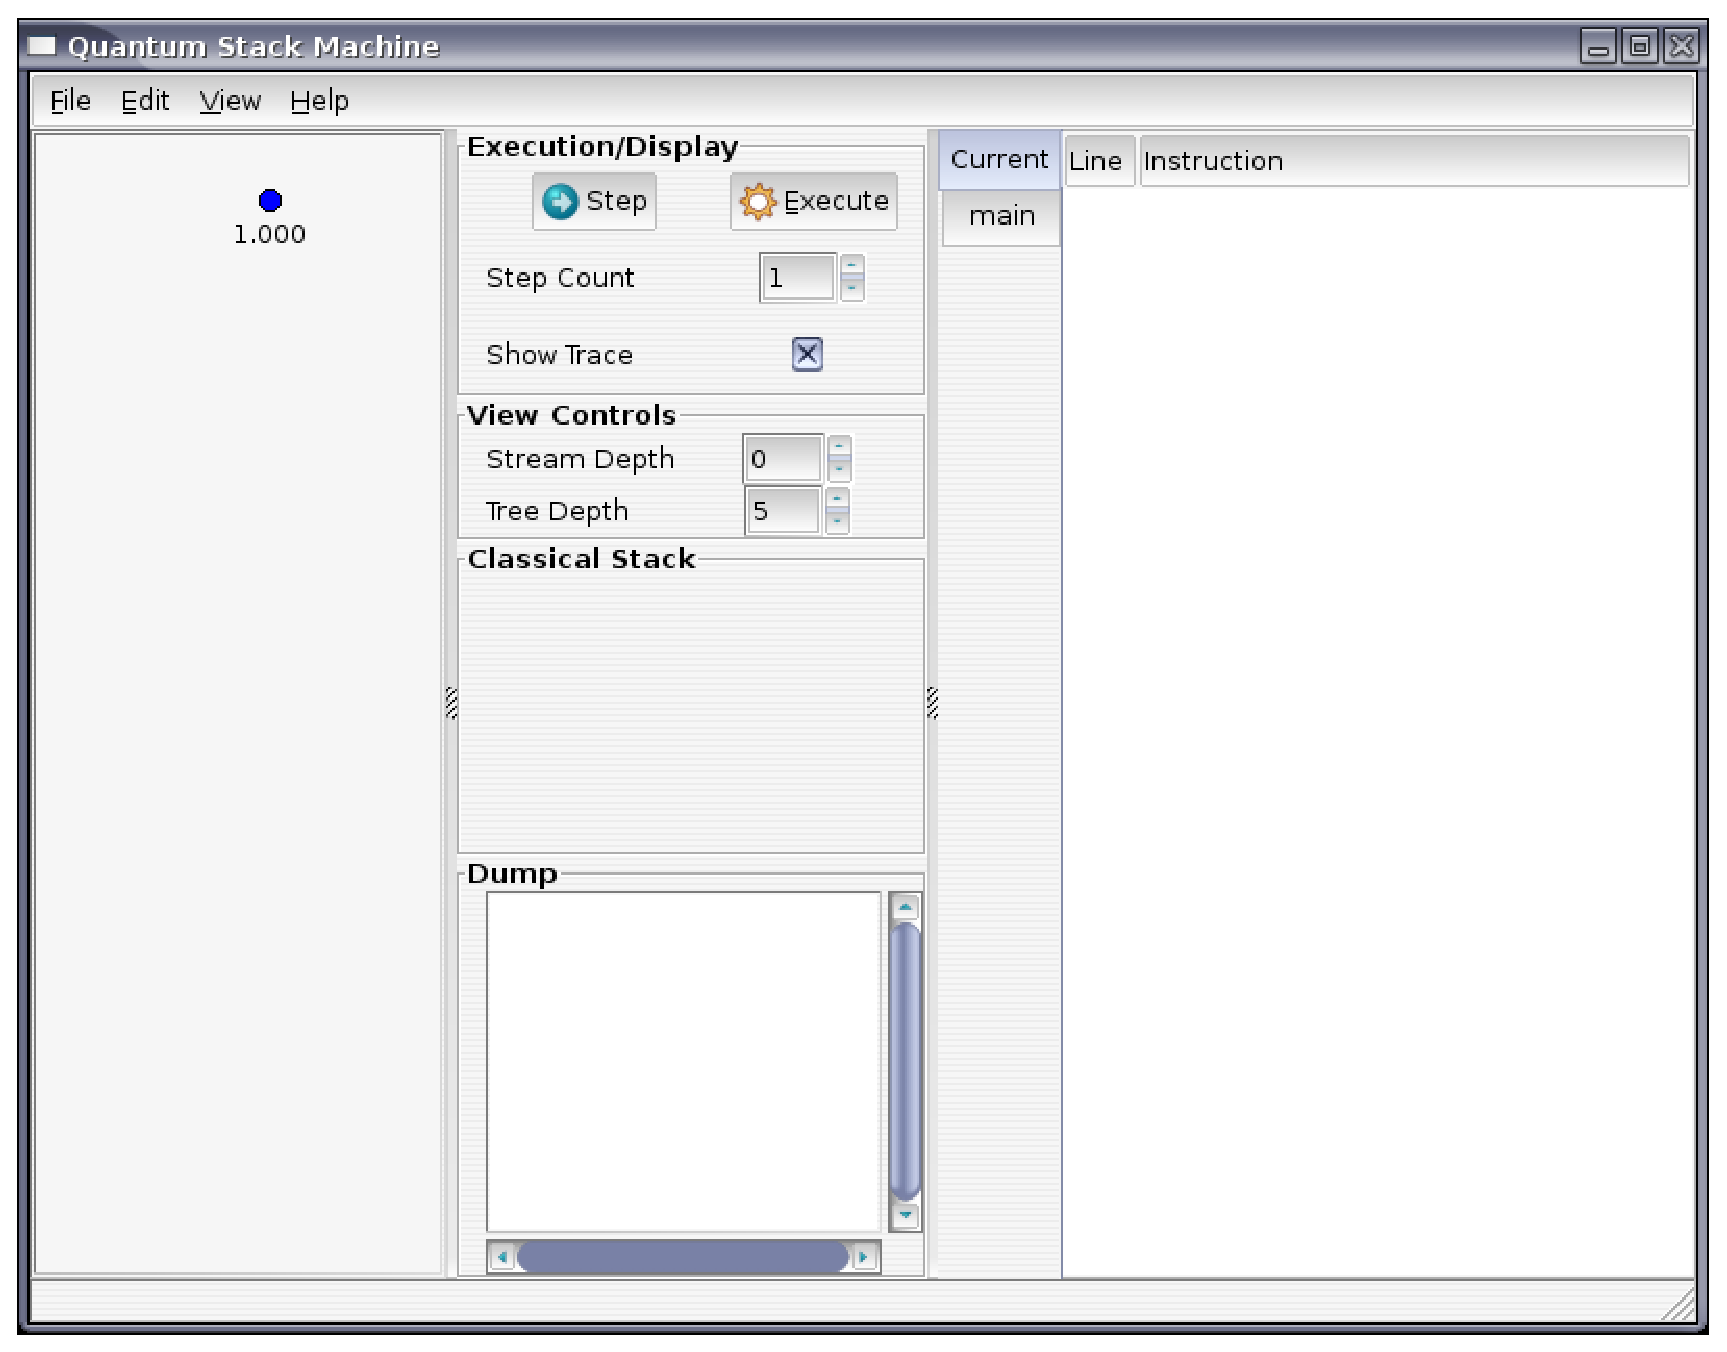
\includegraphics[scale=.5]{images/QSM.startup.eps}
 Just not going to get time to go through it.

\end{document}